%%%% Time-stamp: <2018-03-24 14:05:09 vk>
%% ========================================================================
%%%% Disclaimer
%% ========================================================================
%%
%% created by
%%
%%      Karl Voit
%%

%% ========================================================================
%%%% Basic settings
%% ========================================================================
%% (idea of using newcommands for basic documentclass settings from: Thomas Schlager)

\newcommand{\mypapersize}{A4}
%% e.g., "A4", "letter", "legal", "executive", ...
%% The size of the paper of the resulting PDF file.

\newcommand{\mylaterality}{twoside}
%% "oneside" or "twoside"
%% Either you are creating a document which is printed on both, left pages
%% and right pages (twoside) or you create a document which is printed
%% on right pages only (oneside).

\newcommand{\mydraft}{false}
%% "true" or "false"
%% Use draft mode? If true, included graphics are replaced by empty
%% rectangles (of same size) and overfull boxes (in margin space) are
%% marked with black box (-> easy to spot!)

\newcommand{\myparskip}{half}
%% e.g., "no", "full", "half", ...
%% How to separate paragraphs: indention ("no") or spacing ("half",
%% "full", ...).

\newcommand{\myBCOR}{0mm}
%% Inner binding correction. This value depends on the method which is
%% being used to bind your printed result. Some techniques do not
%% require a binding correction at all ("0mm"), other require for
%% example "5mm". Refer to KOMA script documentation for a detailed
%% explanation what a binding correction is and how to measure it.

\newcommand{\myfontsize}{10pt}
%% e.g., 10pt, 11pt, 12pt
%% The font size of the main text in pt (points).

\newcommand{\mylinespread}{1.05}
%% e.g., 1.0, 1.5, 2.0
%% Line spacing in %/100. For example 1.5 means 150% of the usual line
%% spacing. Please use with caution: 100% ("1.0") is fine because the
%% font was designed for it.

\newcommand{\mylanguage}{ngerman,american}
%% "english,ngerman", "ngerman,english", ...
%% NOTE: The *last* language is the active one!
%% See babel documentation for further details.

%% BibLaTeX-settings: (see biblatex reference for further description)
\newcommand{\mybiblatexstyle}{numeric}
%% e.g., "alphabetic", "authoryear", ...
%% The biblatex style which is being used for referencing. See
%% biblatex documentation for further details and more values.
%%
%% CAUTION: if you change the style, please check for (in)compatible
%%          "biblatex" package options in the file
%%          "template/preamble.tex"! For example: "alphabetic" does
%%          not have an option "dashed=..." and causes an error if it
%%          does not get removed from the list of options.

\newcommand{\mybiblatexdashed}{false}  %% "true" or "false"
%% If true: replace recurring reference authors with a dash.

\newcommand{\mybiblatexbackref}{false}  %% "true" or "false"
%% If true: create backward links from reference to citations.

\newcommand{\mybiblatexfile}{references-biblatex.bib}
%% Name of the biblatex file that holds the references.

\newcommand{\mydispositioncolor}{30,103,182}
%% e.g., "30,103,182" (blue/turquois), "0,0,0" (black), ...
%% Color of the headings and so forth in RGB (red,green,blue) values.
%% NOTE: if you are using "0,0,0" for black, printers might still
%%       recognize pages as color pages. In case this is a problem
%%       (paying for color print-outs vs. paying for b/w-printouts)
%%       please edit file "template/preamble.tex" and change
%%       "\definecolor{DispositionColor}{RGB}{\mydispositioncolor}"
%%       to "\definecolor{DispositionColor}{gray}{0}" and thus
%%       overwriting the value of \mydispositioncolor above.

\newcommand{\mycolorlinks}{true}  %% "true" or "false"
%% Enables or disables colored links (hyperref package).

\newcommand{\mytitlepage}{template/title_Thesis_TU_Graz}
%% Your own or one of following pre-defined title pages:
%% "template/title_plain_maketitle": simple maketitle page
%% "template/title_Diplomarbeit_KF_Uni_Graz.tex": fancy (german) title page for KF Uni Graz
%% "template/title_Thesis_TU_Graz":
%%             titlepage for Graz University of Technology (correct
%%             (old?) Corporate Design) by Karl Voit (2012)
%% "template/title_Thesis_TU_Graz_-_kazemakase":
%%             titlepage for Graz University of Technology
%%             (correct new Corporate Design) by kazemakase (2013):
%%             see https://github.com/novoid/LaTeX-KOMA-template/issues/5
%% "template/title_VWA": titlepage for Vorwissenschaftliche Arbeit

\newcommand{\mytodonotesoptions}{}
%% e.g., "" (empty), "disable", ...
%% Options for the todonotes-package. If "disable", all todonotes will
%% be hidden (including listoftodos).

%% Load main settings for document preamble:
%% Time-stamp: <2018-03-11 14:25:47 vk>
%%%% === Disclaimer: =======================================================
%% created by
%%
%%      Karl Voit
%%
%% using GNU/Linux, GNU Emacs & LaTeX 2e
%%

%doc% %% overriding preamble/preamble.tex %%
%doc% \newcommand{\mylinespread}{1.0}  \newcommand{\mycolorlinks}{true}
%doc% \documentclass[12pt,paper=a4,parskip=half,DIV=calc,oneside,%%
%doc% headinclude,footinclude=false,open=right,bibliography=totoc]{scrartcl}
%doc% \usepackage[utf8]{inputenc}\usepackage[ngerman,american]{babel}\usepackage{scrpage2}
%doc% \usepackage{ifthen}\usepackage{eurosym}\usepackage{xspace}\usepackage[usenames,dvipsnames]{xcolor}
%doc% \usepackage[protrusion=true,factor=900]{microtype}
%doc% \usepackage{enumitem}
%doc% \usepackage[pdftex]{graphicx}
%doc% \usepackage{todonotes}
%doc% \usepackage{dingbat,bbding} %% special characters
%doc% \definecolor{DispositionColor}{RGB}{30,103,182}
%doc%
%doc% \usepackage[backend=biber,style=authoryear,dashed=false,natbib=true,hyperref=true%%
%doc% ]{biblatex}
%doc%
%doc% \addbibresource{references-biblatex.bib} %% remove, if using BibTeX instead of biblatex
%doc%
%doc% %% overriding userdata %%
%doc% \newcommand{\myauthor}{Karl Voit}\newcommand{\mytitle}{LaTeX Template Documentation}
%doc% \newcommand{\mysubject}{A Comprehensive Guide to Use the
%doc% Template from https://github.com/novoid/LaTeX-KOMA-template}
%doc% \newcommand{\mykeywords}{LaTeX, pdflatex, template, documentation, biber, biblatex}
%doc%
%doc% \newcommand{\myLaT}{\LaTeX{}@TUG\xspace}
%doc%
%doc% %% for future use?
%doc% % \usepackage{filecontents}
%doc% % \begin{filecontents}{filename.example}
%doc% %
%doc% % \end{filecontents}
%doc%
%doc%
%doc% %% using existing TeX files %%
%doc% %% Time-stamp: <2015-04-30 17:19:58 vk>
%%%% === Disclaimer: =======================================================
%% created by
%%
%%      Karl Voit
%%
%% using GNU/Linux, GNU Emacs & LaTeX 2e
%%

%doc%
%doc% \section{\texttt{mycommands.tex} --- various definitions}\myinteresting
%doc% \label{sec:mycommands}
%doc%
%doc% In file \verb#template/mycommands.tex# many useful commands are being
%doc% defined. 
%doc% 
%doc% \paragraph{What should I do with this file?} Please take a look at its 
%doc% content to get the most out of your document.
%doc% 

%doc% 
%doc% One of the best advantages of \LaTeX{} compared to \myacro{WYSIWYG} software products is
%doc% the possibility to define and use macros within text. This empowers the user to
%doc% a great extend.  Many things can be defined using \verb#\newcommand{}# and
%doc% automates repeating tasks. It is recommended to use macros not only for
%doc% repetitive tasks but also for separating form from content such as \myacro{CSS}
%doc% does for \myacro{XHTML}. Think of including graphics in your document: after
%doc% writing your book, you might want to change all captions to the upper side of
%doc% each figure. In this case you either have to modify all
%doc% \texttt{includegraphics} commands or you were clever enough to define something
%doc% like \verb#\myfig#\footnote{See below for a detailed description}. Using a
%doc% macro for including graphics enables you to modify the position caption on only
%doc% \emph{one} place: at the definition of the macro.
%doc% 
%doc% The following section describes some macros that came with this document template
%doc% from \myLaT and you are welcome to modify or extend them or to create
%doc% your own macros!
%doc% 

%doc% 
%doc% \subsection{\texttt{myfig} --- including graphics made easy}
%doc% 
%doc% The classic: you can easily add graphics to your document with \verb#\myfig#:
%doc% \begin{verbatim}
%doc%  \myfig{flower}%% filename w/o extension in the folder figures
%doc%        {width=0.7\textwidth}%% maximum width/height, aspect ratio will be kept
%doc%        {This flower was photographed at my home town in 2010}%% caption
%doc%        {Home town flower}%% optional (short) caption for list of figures
%doc%        {fig:flower}%% label
%doc% \end{verbatim}
%doc% 
%doc% There are many advantages of this command (compared to manual
%doc% \texttt{figure} environments and \texttt{includegraphics} commands:
%doc% \begin{itemize}
%doc% \item consistent style throughout the whole document
%doc% \item easy to change; for example move caption on top
%doc% \item much less characters to type (faster, error prone)
%doc% \item less visual clutter in the \TeX{}-files
%doc% \end{itemize}
%doc% 
%doc% 
\newcommand{\myfig}[5]{
%% example:
% \myfig{}%% filename in figures folder
%       {width=0.5\textwidth,height=0.5\textheight}%% maximum width/height, aspect ratio will be kept
%       {}%% caption
%       {}%% optional (short) caption for list of figures
%       {}%% label
\begin{figure}%[htp]
  \centering
  \includegraphics[keepaspectratio,#2]{figures/#1}
  \caption[#4]{#3}
  \label{#5} %% NOTE: always label *after* caption!
\end{figure}
}


%doc% 
%doc% \subsection{\texttt{myclone} --- repeat things!}
%doc% 
%doc% Using \verb#\myclone[42]{foobar}# results the text \enquote{foobar} printed 42 times.
%doc% But you can not only repeat text output with \texttt{myclone}. 
%doc%
%doc% Default argument
%doc% for the optional parameter \enquote{number of times} (like \enquote{42} in the example above) 
%doc% is set to two.
%doc% 
%% \myclone[x]{text}
\newcounter{myclonecnt}
\newcommand{\myclone}[2][2]{%
  \setcounter{myclonecnt}{#1}%
  \whiledo{\value{myclonecnt}>0}{#2\addtocounter{myclonecnt}{-1}}%
}

%old% %d oc% 
%old% %d oc% \subsection{\texttt{fixxme} --- sidemark something as unfinished}
%old% %d oc% 
%old% %d oc% You know it: something has to be fixed and you can not do it right
%old% %d oc% now. In order to \texttt{not} forget about it, you might want to add a
%old% %d oc% note like \verb+\fixxme{check again}+ which inserts a note on the page
%old% %d oc% margin such as this\fixxme{check again} example.
%old% %d oc%
%old% \newcommand{\fixxme}[1]{%%
%old% \textcolor{red}{FIXXME}\marginpar{\textcolor{red}{#1}}%%
%old% }


%%%% End 
%%% Local Variables:
%%% mode: latex
%%% mode: auto-fill
%%% mode: flyspell
%%% eval: (ispell-change-dictionary "en_US")
%%% TeX-master: "../main"
%%% End:
%% vim:foldmethod=expr
%% vim:fde=getline(v\:lnum)=~'^%%%%'?0\:getline(v\:lnum)=~'^%doc.*\ .\\%(sub\\)\\?section{.\\+'?'>1'\:'1':

%doc% %%%% Time-stamp: <2015-08-22 17:20:32 vk>
%%%% === Disclaimer: =======================================================
%% created by
%%
%%      Karl Voit
%%
%% using GNU/Linux, GNU Emacs & LaTeX 2e
%%
%doc%
%doc% \section{\texttt{typographic\_settings.tex} --- Typographic finetuning}
%doc%
%doc% The settings of file \verb#template/typographic_settings.tex# contain
%doc% typographic finetuning related to things mentioned in literature.  The
%doc% settings in this file relates to personal taste and most of all: 
%doc% \emph{typographic experience}. 
%doc% 
%doc% \paragraph{What should I do with this file?} You might as well skip the whole
%doc% file by excluding the \verb#%%%% Time-stamp: <2015-08-22 17:20:32 vk>
%%%% === Disclaimer: =======================================================
%% created by
%%
%%      Karl Voit
%%
%% using GNU/Linux, GNU Emacs & LaTeX 2e
%%
%doc%
%doc% \section{\texttt{typographic\_settings.tex} --- Typographic finetuning}
%doc%
%doc% The settings of file \verb#template/typographic_settings.tex# contain
%doc% typographic finetuning related to things mentioned in literature.  The
%doc% settings in this file relates to personal taste and most of all: 
%doc% \emph{typographic experience}. 
%doc% 
%doc% \paragraph{What should I do with this file?} You might as well skip the whole
%doc% file by excluding the \verb#\input{template/typographic_settings.tex}# command
%doc% in \texttt{main.tex}.  For standard usage it is recommended to stay with the
%doc% default settings.
%doc% 
%doc% 
%% ========================================================================

%doc%
%doc% Some basic microtypographic settings are provided by the
%doc% \texttt{microtype}
%doc% package\footnote{\url{http://ctan.org/pkg/microtype}}. This template
%doc% uses the rather conservative package parameters: \texttt{protrusion=true,factor=900}.
\usepackage[protrusion=true,factor=900]{microtype}

%doc%
%doc% \subsection{French spacing}
%doc%
%doc% \paragraph{Why?} see~\textcite[p.\,28, p.\,30]{Bringhurst1993}: `2.1.4 Use a single word space between sentences.'
%doc%
%doc% \paragraph{How?} see~\textcite[p.\,185]{Eijkhout2008}:\\
%doc% \verb#\frenchspacing  %% Macro to switch off extra space after punctuation.# \\
\frenchspacing  %% Macro to switch off extra space after punctuation.
%doc%
%doc% Note: This setting might be default for \myacro{KOMA} script.
%doc%


%doc%
%doc% \subsection{Font}
%doc% 
%doc% This template is using the Palatino font (package \texttt{mathpazo}) which results
%doc% in a legible document and matching mathematical fonts for printout.
%doc% 
%doc% It is highly recommended that you either stick to the Palatino font or use the
%doc% \LaTeX{} default fonts (by removing the package \texttt{mathpazo}).
%doc% 
%doc% Chosing different fonts is not
%doc% an easy task. Please leave this to people with good knowledge on this subject.
%doc% 
%doc% One valid reason to change the default fonts is when your document is mainly
%doc% read on a computer screen. In this case it is recommended to switch to a font
%doc% \textsf{which is sans-serif like this}. This template contains several alternative
%doc% font packages which can be activated in this file.
%doc% 

% for changing the default font, please go to the next subsection!

%doc%
%doc% \subsection{Text figures}
%doc% 
%doc% \ldots also called old style numbers such as 0123456789. 
%doc% (German: \enquote{Mediäval\-ziffern\footnote{\url{https://secure.wikimedia.org/wikibooks/de/wiki/LaTeX-W\%C3\%B6rterbuch:\_Medi\%C3\%A4valziffern}}})
%doc% \paragraph{Why?} see~\textcite[p.\,44f]{Bringhurst1993}: 
%doc% \begin{quote}
%doc% `3.2.1 If the font includes both text figures and titling figures, use
%doc%  titling figures only with full caps, and text figures in all other
%doc%  circumstances.'
%doc% \end{quote}
%doc% 
%doc% \paragraph{How?} 
%doc% Quoted from Wikibooks\footnote{\url{https://secure.wikimedia.org/wikibooks/en/wiki/LaTeX/Formatting\#Text\_figures\_.28.22old\_style.22\_numerals.29}}:
%doc% \begin{quote}
%doc% Some fonts do not have text figures built in; the textcomp package attempts to
%doc% remedy this by effectively generating text figures from the currently-selected
%doc% font. Put \verb#\usepackage{textcomp}# in your preamble. textcomp also allows you to
%doc% use decimal points, properly formatted dollar signs, etc. within
%doc% \verb#\oldstylenums{}#.
%doc% \end{quote}
%doc% \ldots but proposed \LaTeX{} method does not work out well. Instead use:\\
%doc% \verb#\usepackage{hfoldsty}#  (enables text figures using additional font) or \\
%doc% \verb#\usepackage[sc,osf]{mathpazo}# (switches to Palatino font with small caps and old style figures enabled).
%doc%
%\usepackage{hfoldsty}  %% enables text figures using additional font
%% ... OR use ...
\usepackage[sc,osf]{mathpazo} %% switches to Palatino with small caps and old style figures

%% Font selection from:
%%     http://www.matthiaspospiech.de/latex/vorlagen/allgemein/preambel/fonts/
%% use following lines *instead* of the mathpazo package above:
%% ===== Serif =========================================================
%% for Computer Modern (LaTeX default font), simply remove the mathpazo above
%\usepackage{charter}\linespread{1.05} %% Charter
%\usepackage{bookman}                  %% Bookman (laedt Avant Garde !!)
%\usepackage{newcent}                  %% New Century Schoolbook (laedt Avant Garde !!)
%% ===== Sans Serif ====================================================
%\renewcommand{\familydefault}{\sfdefault}  %% this one in *combination* with the default mathpazo package
%\usepackage{cmbright}                  %% CM-Bright (eigntlich eine Familie)
%\usepackage{tpslifonts}                %% tpslifonts % Font for Slides


%doc% 
%doc% \subsection{\texttt{myacro} --- Abbrevations using \textsc{small caps}}\myinteresting
%doc% \label{sec:myacro}
%doc% 
%doc% \paragraph{Why?} see~\textcite[p.\,45f]{Bringhurst1993}: `3.2.2 For abbrevations and
%doc% acronyms in the midst of normal text, use spaced small caps.'
%doc% 
%doc% \paragraph{How?} Using the predefined macro \verb#\myacro{}# for things like
%doc% \myacro{UNO} or \myacro{UNESCO} using \verb#\myacro{UNO}# or \verb#\myacro{UNESCO}#.
%doc% 
\DeclareRobustCommand{\myacro}[1]{\textsc{\lowercase{#1}}} %%  abbrevations using small caps


%doc% 
%doc% \subsection{Colorized headings and links}
%doc% 
%doc% This document template is able to generate an output that uses colorized
%doc% headings, captions, page numbers, and links. The color named `DispositionColor'
%doc% used in this document is defined near the definition of package \texttt{color}
%doc% in the preamble (see section~\ref{subsec:miscpackages}). The changes required
%doc% for headings, page numbers, and captions are defined here.
%doc% 
%doc% Settings for colored links are handled by the definitions of the
%doc% \texttt{hyperref} package (see section~\ref{sec:pdf}).
%doc% 
\setheadsepline{.4pt}[\color{DispositionColor}]
\renewcommand{\headfont}{\normalfont\sffamily\color{DispositionColor}}
\renewcommand{\pnumfont}{\normalfont\sffamily\color{DispositionColor}}
\addtokomafont{disposition}{\color{DispositionColor}}
\addtokomafont{caption}{\color{DispositionColor}\footnotesize}
\addtokomafont{captionlabel}{\color{DispositionColor}}

%doc% 
%doc% \subsection{No figures or tables below footnotes}
%doc% 
%doc% \LaTeX{} places floating environments below footnotes if \texttt{b}
%doc% (bottom) is used as (default) placement algorithm. This is certainly
%doc% not appealing for most people and is deactivated in this template by
%doc% using the package \texttt{footmisc} with its option \texttt{bottom}.
%doc% 
%% see also: http://www.komascript.de/node/858 (German description)
\usepackage[bottom]{footmisc}

%doc% 
%doc% \subsection{Spacings of list environments}
%doc% 
%doc% By default, \LaTeX{} is using vertical spaces between items of enumerate, 
%doc% itemize and description environments. This is fine for multi-line items.
%doc% Many times, the user does just write single-line items where the larger
%doc% vertical space is inappropriate. The \href{http://ctan.org/pkg/enumitem}{enumitem}
%doc% package provides replacements for the pre-defined list environments and
%doc% offers many options to modify their appearances.
%doc% This template is using the package option for \texttt{noitemsep} which
%doc% mimimizes the vertical space between list items.
%doc% 
\usepackage{enumitem}
\setlist{noitemsep}   %% kills the space between items

%doc% 
%doc% \subsection{\texttt{csquotes} --- Correct quotation marks}\myinteresting
%doc% \label{sub:csquotes}
%doc% 
%doc% \emph{Never} use quotation marks found on your keyboard.
%doc% They end up in strange characters or false looking quotation marks.
%doc% 
%doc% In \LaTeX{} you are able to use typographically correct quotation marks. The package 
%doc% \href{http://www.ctan.org/pkg/csquotes}{\texttt{csquotes}} offers you with 
%doc% \verb#\enquote{foobar}# a command to get correct quotation marks around \enquote{foobar}.
%doc% Please do check the package options in order to modify
%doc% its settings according to the language used\footnote{most of the time in 
%doc% combination with the language set in the options of the \texttt{babel} package}.
%doc% 
%doc% \href{http://www.ctan.org/pkg/csquotes}{\texttt{csquotes}} is also recommended 
%doc% by \texttt{biblatex} (see Section~\ref{sec:references}). 
\usepackage[babel=true,strict=true,english=american,german=guillemets]{csquotes}

%doc% 
%doc% \subsection{Line spread}
%doc% 
%doc% If you have to enlarge the distance between two lines of text, you can
%doc% increase it using the \texttt{\mylinespread} command in \texttt{main.tex}. By default, it is
%doc% deactivated (set to 100~percent). Modify only with caution since it influences the
%doc% page layout and could lead to ugly looking documents.
\linespread{\mylinespread}

%doc% 
%doc% \subsection{Optional: Lines above and below the chapter head}
%doc% 
%doc% This is not quite something typographic but rather a matter of taste.
%doc% \myacro{KOMA} Script offers \href{http://www.komascript.de/node/24}{a method to
%doc% add lines above and below chapter head} which is disabled by
%doc% default. If you want to enable this feature, remove corresponding
%doc% comment characters from the settings.
%doc% 
%% Source: http://www.komascript.de/node/24
%disabled% %% 1st get a new command
%disabled% \newcommand*{\ORIGchapterheadstartvskip}{}%
%disabled% %% 2nd save the original definition to the new command
%disabled% \let\ORIGchapterheadstartvskip=\chapterheadstartvskip
%disabled% %% 3rd redefine the command using the saved original command
%disabled% \renewcommand*{\chapterheadstartvskip}{%
%disabled%   \ORIGchapterheadstartvskip
%disabled%   {%
%disabled%     \setlength{\parskip}{0pt}%
%disabled%     \noindent\color{DispositionColor}\rule[.3\baselineskip]{\linewidth}{1pt}\par
%disabled%   }%
%disabled% }
%disabled% %% see above
%disabled% \newcommand*{\ORIGchapterheadendvskip}{}%
%disabled% \let\ORIGchapterheadendvskip=\chapterheadendvskip
%disabled% \renewcommand*{\chapterheadendvskip}{%
%disabled%   {%
%disabled%     \setlength{\parskip}{0pt}%
%disabled%     \noindent\color{DispositionColor}\rule[.3\baselineskip]{\linewidth}{1pt}\par
%disabled%   }%
%disabled%   \ORIGchapterheadendvskip
%disabled% }

%doc% 
%doc% \subsection{Optional: Chapter thumbs}
%doc% 
%doc% This is not quite something typographic but rather a matter of taste.
%doc% \myacro{KOMA} Script offers \href{http://www.komascript.de/chapterthumbs-example}{a method to
%doc% add chapter thumbs} (in combination with the package \texttt{scrpage2}) which is disabled by
%doc% default. If you want to enable this feature, remove corresponding
%doc% comment characters from the settings.
%doc% 
%disabled% \makeatletter
%disabled% % Safty first
%disabled% \@ifundefined{chapter}{\let\chapter\undefined
%disabled%   \chapter must be defined to use chapter thumbs!}{%
%disabled%  
%disabled% % Two new commands for the width and height of the boxes with the
%disabled% % chapter number at the thumbs (use of commands instead of lengths
%disabled% % for sparing registers)
%disabled% \newcommand*{\chapterthumbwidth}{2em}
%disabled% \newcommand*{\chapterthumbheight}{1em}
%disabled%  
%disabled% % Two new commands for the colors of the box background and the
%disabled% % chapter numbers of the thumbs
%disabled% \newcommand*{\chapterthumbboxcolor}{black}
%disabled% \newcommand*{\chapterthumbtextcolor}{white}
%disabled%  
%disabled% % New command to set a chapter thumb. I'm using a group at this
%disabled% % command, because I'm changing the temporary dimension \@tempdima
%disabled% \newcommand*{\putchapterthumb}{%
%disabled%   \begingroup
%disabled%     \Large
%disabled%     % calculate the horizontal possition of the right paper border
%disabled%     % (I ignore \hoffset, because I interprete \hoffset moves the page
%disabled%     % at the paper e.g. if you are using cropmarks)
%disabled%     \setlength{\@tempdima}{\@oddheadshift}% (internal from scrpage2)
%disabled%     \setlength{\@tempdima}{-\@tempdima}%
%disabled%     \addtolength{\@tempdima}{\paperwidth}%
%disabled%     \addtolength{\@tempdima}{-\oddsidemargin}%
%disabled%     \addtolength{\@tempdima}{-1in}%
%disabled%     % putting the thumbs should not change the horizontal
%disabled%     % possition
%disabled%     \rlap{%
%disabled%       % move to the calculated horizontal possition
%disabled%       \hspace*{\@tempdima}%
%disabled%       % putting the thumbs should not change the vertical
%disabled%       % possition
%disabled%       \vbox to 0pt{%
%disabled%         % calculate the vertical possition of the thumbs (I ignore
%disabled%         % \voffset for the same reasons told above)
%disabled%         \setlength{\@tempdima}{\chapterthumbwidth}%
%disabled%         \multiply\@tempdima by\value{chapter}%
%disabled%         \addtolength{\@tempdima}{-\chapterthumbwidth}%
%disabled%         \addtolength{\@tempdima}{-\baselineskip}%
%disabled%         % move to the calculated vertical possition
%disabled%         \vspace*{\@tempdima}%
%disabled%         % put the thumbs left so the current horizontal possition
%disabled%         \llap{%
%disabled%           % and rotate them
%disabled%           \rotatebox{90}{\colorbox{\chapterthumbboxcolor}{%
%disabled%               \parbox[c][\chapterthumbheight][c]{\chapterthumbwidth}{%
%disabled%                 \centering
%disabled%                 \textcolor{\chapterthumbtextcolor}{%
%disabled%                   \strut\thechapter}\\
%disabled%               }%
%disabled%             }%
%disabled%           }%
%disabled%         }%
%disabled%         % avoid overfull \vbox messages
%disabled%         \vss
%disabled%       }%
%disabled%     }%
%disabled%   \endgroup
%disabled% }
%disabled%  
%disabled% % New command, which works like \lohead but also puts the thumbs (you
%disabled% % cannot use \ihead with this definition but you may change this, if
%disabled% % you use more internal scrpage2 commands)
%disabled% \newcommand*{\loheadwithchapterthumbs}[2][]{%
%disabled%   \lohead[\putchapterthumb#1]{\putchapterthumb#2}%
%disabled% }
%disabled%  
%disabled% % initial use
%disabled% \loheadwithchapterthumbs{}
%disabled% \pagestyle{scrheadings}
%disabled%  
%disabled% }
%disabled% \makeatother

%%%% END
%%% Local Variables:
%%% mode: latex
%%% mode: auto-fill
%%% mode: flyspell
%%% eval: (ispell-change-dictionary "en_US")
%%% TeX-master: "../main"
%%% End:
%% vim:foldmethod=expr
%% vim:fde=getline(v\:lnum)=~'^%%%%'?0\:getline(v\:lnum)=~'^%doc.*\ .\\%(sub\\)\\?section{.\\+'?'>1'\:'1':
# command
%doc% in \texttt{main.tex}.  For standard usage it is recommended to stay with the
%doc% default settings.
%doc% 
%doc% 
%% ========================================================================

%doc%
%doc% Some basic microtypographic settings are provided by the
%doc% \texttt{microtype}
%doc% package\footnote{\url{http://ctan.org/pkg/microtype}}. This template
%doc% uses the rather conservative package parameters: \texttt{protrusion=true,factor=900}.
\usepackage[protrusion=true,factor=900]{microtype}

%doc%
%doc% \subsection{French spacing}
%doc%
%doc% \paragraph{Why?} see~\textcite[p.\,28, p.\,30]{Bringhurst1993}: `2.1.4 Use a single word space between sentences.'
%doc%
%doc% \paragraph{How?} see~\textcite[p.\,185]{Eijkhout2008}:\\
%doc% \verb#\frenchspacing  %% Macro to switch off extra space after punctuation.# \\
\frenchspacing  %% Macro to switch off extra space after punctuation.
%doc%
%doc% Note: This setting might be default for \myacro{KOMA} script.
%doc%


%doc%
%doc% \subsection{Font}
%doc% 
%doc% This template is using the Palatino font (package \texttt{mathpazo}) which results
%doc% in a legible document and matching mathematical fonts for printout.
%doc% 
%doc% It is highly recommended that you either stick to the Palatino font or use the
%doc% \LaTeX{} default fonts (by removing the package \texttt{mathpazo}).
%doc% 
%doc% Chosing different fonts is not
%doc% an easy task. Please leave this to people with good knowledge on this subject.
%doc% 
%doc% One valid reason to change the default fonts is when your document is mainly
%doc% read on a computer screen. In this case it is recommended to switch to a font
%doc% \textsf{which is sans-serif like this}. This template contains several alternative
%doc% font packages which can be activated in this file.
%doc% 

% for changing the default font, please go to the next subsection!

%doc%
%doc% \subsection{Text figures}
%doc% 
%doc% \ldots also called old style numbers such as 0123456789. 
%doc% (German: \enquote{Mediäval\-ziffern\footnote{\url{https://secure.wikimedia.org/wikibooks/de/wiki/LaTeX-W\%C3\%B6rterbuch:\_Medi\%C3\%A4valziffern}}})
%doc% \paragraph{Why?} see~\textcite[p.\,44f]{Bringhurst1993}: 
%doc% \begin{quote}
%doc% `3.2.1 If the font includes both text figures and titling figures, use
%doc%  titling figures only with full caps, and text figures in all other
%doc%  circumstances.'
%doc% \end{quote}
%doc% 
%doc% \paragraph{How?} 
%doc% Quoted from Wikibooks\footnote{\url{https://secure.wikimedia.org/wikibooks/en/wiki/LaTeX/Formatting\#Text\_figures\_.28.22old\_style.22\_numerals.29}}:
%doc% \begin{quote}
%doc% Some fonts do not have text figures built in; the textcomp package attempts to
%doc% remedy this by effectively generating text figures from the currently-selected
%doc% font. Put \verb#\usepackage{textcomp}# in your preamble. textcomp also allows you to
%doc% use decimal points, properly formatted dollar signs, etc. within
%doc% \verb#\oldstylenums{}#.
%doc% \end{quote}
%doc% \ldots but proposed \LaTeX{} method does not work out well. Instead use:\\
%doc% \verb#\usepackage{hfoldsty}#  (enables text figures using additional font) or \\
%doc% \verb#\usepackage[sc,osf]{mathpazo}# (switches to Palatino font with small caps and old style figures enabled).
%doc%
%\usepackage{hfoldsty}  %% enables text figures using additional font
%% ... OR use ...
\usepackage[sc,osf]{mathpazo} %% switches to Palatino with small caps and old style figures

%% Font selection from:
%%     http://www.matthiaspospiech.de/latex/vorlagen/allgemein/preambel/fonts/
%% use following lines *instead* of the mathpazo package above:
%% ===== Serif =========================================================
%% for Computer Modern (LaTeX default font), simply remove the mathpazo above
%\usepackage{charter}\linespread{1.05} %% Charter
%\usepackage{bookman}                  %% Bookman (laedt Avant Garde !!)
%\usepackage{newcent}                  %% New Century Schoolbook (laedt Avant Garde !!)
%% ===== Sans Serif ====================================================
%\renewcommand{\familydefault}{\sfdefault}  %% this one in *combination* with the default mathpazo package
%\usepackage{cmbright}                  %% CM-Bright (eigntlich eine Familie)
%\usepackage{tpslifonts}                %% tpslifonts % Font for Slides


%doc% 
%doc% \subsection{\texttt{myacro} --- Abbrevations using \textsc{small caps}}\myinteresting
%doc% \label{sec:myacro}
%doc% 
%doc% \paragraph{Why?} see~\textcite[p.\,45f]{Bringhurst1993}: `3.2.2 For abbrevations and
%doc% acronyms in the midst of normal text, use spaced small caps.'
%doc% 
%doc% \paragraph{How?} Using the predefined macro \verb#\myacro{}# for things like
%doc% \myacro{UNO} or \myacro{UNESCO} using \verb#\myacro{UNO}# or \verb#\myacro{UNESCO}#.
%doc% 
\DeclareRobustCommand{\myacro}[1]{\textsc{\lowercase{#1}}} %%  abbrevations using small caps


%doc% 
%doc% \subsection{Colorized headings and links}
%doc% 
%doc% This document template is able to generate an output that uses colorized
%doc% headings, captions, page numbers, and links. The color named `DispositionColor'
%doc% used in this document is defined near the definition of package \texttt{color}
%doc% in the preamble (see section~\ref{subsec:miscpackages}). The changes required
%doc% for headings, page numbers, and captions are defined here.
%doc% 
%doc% Settings for colored links are handled by the definitions of the
%doc% \texttt{hyperref} package (see section~\ref{sec:pdf}).
%doc% 
\setheadsepline{.4pt}[\color{DispositionColor}]
\renewcommand{\headfont}{\normalfont\sffamily\color{DispositionColor}}
\renewcommand{\pnumfont}{\normalfont\sffamily\color{DispositionColor}}
\addtokomafont{disposition}{\color{DispositionColor}}
\addtokomafont{caption}{\color{DispositionColor}\footnotesize}
\addtokomafont{captionlabel}{\color{DispositionColor}}

%doc% 
%doc% \subsection{No figures or tables below footnotes}
%doc% 
%doc% \LaTeX{} places floating environments below footnotes if \texttt{b}
%doc% (bottom) is used as (default) placement algorithm. This is certainly
%doc% not appealing for most people and is deactivated in this template by
%doc% using the package \texttt{footmisc} with its option \texttt{bottom}.
%doc% 
%% see also: http://www.komascript.de/node/858 (German description)
\usepackage[bottom]{footmisc}

%doc% 
%doc% \subsection{Spacings of list environments}
%doc% 
%doc% By default, \LaTeX{} is using vertical spaces between items of enumerate, 
%doc% itemize and description environments. This is fine for multi-line items.
%doc% Many times, the user does just write single-line items where the larger
%doc% vertical space is inappropriate. The \href{http://ctan.org/pkg/enumitem}{enumitem}
%doc% package provides replacements for the pre-defined list environments and
%doc% offers many options to modify their appearances.
%doc% This template is using the package option for \texttt{noitemsep} which
%doc% mimimizes the vertical space between list items.
%doc% 
\usepackage{enumitem}
\setlist{noitemsep}   %% kills the space between items

%doc% 
%doc% \subsection{\texttt{csquotes} --- Correct quotation marks}\myinteresting
%doc% \label{sub:csquotes}
%doc% 
%doc% \emph{Never} use quotation marks found on your keyboard.
%doc% They end up in strange characters or false looking quotation marks.
%doc% 
%doc% In \LaTeX{} you are able to use typographically correct quotation marks. The package 
%doc% \href{http://www.ctan.org/pkg/csquotes}{\texttt{csquotes}} offers you with 
%doc% \verb#\enquote{foobar}# a command to get correct quotation marks around \enquote{foobar}.
%doc% Please do check the package options in order to modify
%doc% its settings according to the language used\footnote{most of the time in 
%doc% combination with the language set in the options of the \texttt{babel} package}.
%doc% 
%doc% \href{http://www.ctan.org/pkg/csquotes}{\texttt{csquotes}} is also recommended 
%doc% by \texttt{biblatex} (see Section~\ref{sec:references}). 
\usepackage[babel=true,strict=true,english=american,german=guillemets]{csquotes}

%doc% 
%doc% \subsection{Line spread}
%doc% 
%doc% If you have to enlarge the distance between two lines of text, you can
%doc% increase it using the \texttt{\mylinespread} command in \texttt{main.tex}. By default, it is
%doc% deactivated (set to 100~percent). Modify only with caution since it influences the
%doc% page layout and could lead to ugly looking documents.
\linespread{\mylinespread}

%doc% 
%doc% \subsection{Optional: Lines above and below the chapter head}
%doc% 
%doc% This is not quite something typographic but rather a matter of taste.
%doc% \myacro{KOMA} Script offers \href{http://www.komascript.de/node/24}{a method to
%doc% add lines above and below chapter head} which is disabled by
%doc% default. If you want to enable this feature, remove corresponding
%doc% comment characters from the settings.
%doc% 
%% Source: http://www.komascript.de/node/24
%disabled% %% 1st get a new command
%disabled% \newcommand*{\ORIGchapterheadstartvskip}{}%
%disabled% %% 2nd save the original definition to the new command
%disabled% \let\ORIGchapterheadstartvskip=\chapterheadstartvskip
%disabled% %% 3rd redefine the command using the saved original command
%disabled% \renewcommand*{\chapterheadstartvskip}{%
%disabled%   \ORIGchapterheadstartvskip
%disabled%   {%
%disabled%     \setlength{\parskip}{0pt}%
%disabled%     \noindent\color{DispositionColor}\rule[.3\baselineskip]{\linewidth}{1pt}\par
%disabled%   }%
%disabled% }
%disabled% %% see above
%disabled% \newcommand*{\ORIGchapterheadendvskip}{}%
%disabled% \let\ORIGchapterheadendvskip=\chapterheadendvskip
%disabled% \renewcommand*{\chapterheadendvskip}{%
%disabled%   {%
%disabled%     \setlength{\parskip}{0pt}%
%disabled%     \noindent\color{DispositionColor}\rule[.3\baselineskip]{\linewidth}{1pt}\par
%disabled%   }%
%disabled%   \ORIGchapterheadendvskip
%disabled% }

%doc% 
%doc% \subsection{Optional: Chapter thumbs}
%doc% 
%doc% This is not quite something typographic but rather a matter of taste.
%doc% \myacro{KOMA} Script offers \href{http://www.komascript.de/chapterthumbs-example}{a method to
%doc% add chapter thumbs} (in combination with the package \texttt{scrpage2}) which is disabled by
%doc% default. If you want to enable this feature, remove corresponding
%doc% comment characters from the settings.
%doc% 
%disabled% \makeatletter
%disabled% % Safty first
%disabled% \@ifundefined{chapter}{\let\chapter\undefined
%disabled%   \chapter must be defined to use chapter thumbs!}{%
%disabled%  
%disabled% % Two new commands for the width and height of the boxes with the
%disabled% % chapter number at the thumbs (use of commands instead of lengths
%disabled% % for sparing registers)
%disabled% \newcommand*{\chapterthumbwidth}{2em}
%disabled% \newcommand*{\chapterthumbheight}{1em}
%disabled%  
%disabled% % Two new commands for the colors of the box background and the
%disabled% % chapter numbers of the thumbs
%disabled% \newcommand*{\chapterthumbboxcolor}{black}
%disabled% \newcommand*{\chapterthumbtextcolor}{white}
%disabled%  
%disabled% % New command to set a chapter thumb. I'm using a group at this
%disabled% % command, because I'm changing the temporary dimension \@tempdima
%disabled% \newcommand*{\putchapterthumb}{%
%disabled%   \begingroup
%disabled%     \Large
%disabled%     % calculate the horizontal possition of the right paper border
%disabled%     % (I ignore \hoffset, because I interprete \hoffset moves the page
%disabled%     % at the paper e.g. if you are using cropmarks)
%disabled%     \setlength{\@tempdima}{\@oddheadshift}% (internal from scrpage2)
%disabled%     \setlength{\@tempdima}{-\@tempdima}%
%disabled%     \addtolength{\@tempdima}{\paperwidth}%
%disabled%     \addtolength{\@tempdima}{-\oddsidemargin}%
%disabled%     \addtolength{\@tempdima}{-1in}%
%disabled%     % putting the thumbs should not change the horizontal
%disabled%     % possition
%disabled%     \rlap{%
%disabled%       % move to the calculated horizontal possition
%disabled%       \hspace*{\@tempdima}%
%disabled%       % putting the thumbs should not change the vertical
%disabled%       % possition
%disabled%       \vbox to 0pt{%
%disabled%         % calculate the vertical possition of the thumbs (I ignore
%disabled%         % \voffset for the same reasons told above)
%disabled%         \setlength{\@tempdima}{\chapterthumbwidth}%
%disabled%         \multiply\@tempdima by\value{chapter}%
%disabled%         \addtolength{\@tempdima}{-\chapterthumbwidth}%
%disabled%         \addtolength{\@tempdima}{-\baselineskip}%
%disabled%         % move to the calculated vertical possition
%disabled%         \vspace*{\@tempdima}%
%disabled%         % put the thumbs left so the current horizontal possition
%disabled%         \llap{%
%disabled%           % and rotate them
%disabled%           \rotatebox{90}{\colorbox{\chapterthumbboxcolor}{%
%disabled%               \parbox[c][\chapterthumbheight][c]{\chapterthumbwidth}{%
%disabled%                 \centering
%disabled%                 \textcolor{\chapterthumbtextcolor}{%
%disabled%                   \strut\thechapter}\\
%disabled%               }%
%disabled%             }%
%disabled%           }%
%disabled%         }%
%disabled%         % avoid overfull \vbox messages
%disabled%         \vss
%disabled%       }%
%disabled%     }%
%disabled%   \endgroup
%disabled% }
%disabled%  
%disabled% % New command, which works like \lohead but also puts the thumbs (you
%disabled% % cannot use \ihead with this definition but you may change this, if
%disabled% % you use more internal scrpage2 commands)
%disabled% \newcommand*{\loheadwithchapterthumbs}[2][]{%
%disabled%   \lohead[\putchapterthumb#1]{\putchapterthumb#2}%
%disabled% }
%disabled%  
%disabled% % initial use
%disabled% \loheadwithchapterthumbs{}
%disabled% \pagestyle{scrheadings}
%disabled%  
%disabled% }
%disabled% \makeatother

%%%% END
%%% Local Variables:
%%% mode: latex
%%% mode: auto-fill
%%% mode: flyspell
%%% eval: (ispell-change-dictionary "en_US")
%%% TeX-master: "../main"
%%% End:
%% vim:foldmethod=expr
%% vim:fde=getline(v\:lnum)=~'^%%%%'?0\:getline(v\:lnum)=~'^%doc.*\ .\\%(sub\\)\\?section{.\\+'?'>1'\:'1':

%doc% %%%% Time-stamp: <2018-03-11 14:31:45 vk>
%%%% === Disclaimer: =======================================================
%% created by
%%
%%      Karl Voit
%%
%% using GNU/Linux, GNU Emacs & LaTeX 2e
%%

%doc%
%doc% \section{\texttt{pdf\_settings.tex} --- Settings related to PDF output}
%doc% \label{sec:pdf}
%doc%
%doc% The file \verb#template/pdf_settings.tex# basically contains the definitions for
%doc% the \href{http://tug.org/applications/hyperref/}{\texttt{hyperref} package}
%doc% including the
%doc% \href{http://www.ctan.org/tex-archive/macros/latex/required/graphics/}{\texttt{graphicx}
%doc% package}. Since these settings should be the last things of any \LaTeX{}
%doc% preamble, they got their own \TeX{} file which is included in \texttt{main.tex}.
%doc%
%doc% \paragraph{What should I do with this file?} The settings in this file are
%doc% important for \myacro{PDF} output and including graphics. Do not exclude the
%doc% related \texttt{input} command in \texttt{main.tex}. But you might want to
%doc% modify some settings after you read the
%doc% \href{http://tug.org/applications/hyperref/}{documentation of the \texttt{hyperref} package}.
%doc%


%% Fix positioning of images in PDF viewers. (disabled by
%% default; see https://github.com/novoid/LaTeX-KOMA-template/issues/4
%% for more information)
%% I do not have time to read about possible side-effect of this
%% package for now.
% \usepackage[hypcap]{caption}

%% Declarations of hyperref should be the last definitions of the preamble:
%% FIXXME: black-and-white-version for printing!

\pdfcompresslevel=9

\usepackage[%
unicode=true, % loads with unicode support
%a4paper=true, %
%pdftex=true, %
backref, %
pagebackref=false, % creates backward references too
bookmarks=true, % generate bookmarks in PDF files
bookmarksopen=false, % when starting with AcrobatReader, the Bookmarkcolumn is opened
pdfpagemode=UseNone,% None, UseOutlines, UseThumbs, FullScreen
plainpages=false, % correct, if pdflatex complains: ``destination with same identifier already exists''
%% colors: https://secure.wikimedia.org/wikibooks/en/wiki/LaTeX/Colors
urlcolor=DispositionColor, %%
linkcolor=DispositionColor, %%
%pagecolor=DispositionColor, %%
citecolor=DispositionColor, %%
anchorcolor=DispositionColor, %%
colorlinks=\mycolorlinks, % turn on/off colored links (on: better for
                          % on-screen reading; off: better for printout versions)
]{hyperref}

%% all strings need to be loaded after hyperref was loaded with unicode support
%% if not the field is garbled in the output for characters like ČŽĆŠĐ
\hypersetup{
pdftitle={\mytitle}, %
pdfauthor={\myauthor}, %
pdfsubject={\mysubject}, %
pdfcreator={Accomplished with: pdfLaTeX, biber, and hyperref-package. No animals, MS-EULA or BSA-rules were harmed.},
pdfproducer={\myauthor},
pdfkeywords={\mykeywords}
}

%\DeclareGraphicsExtensions{.pdf}

%%%% END
%%% Local Variables:
%%% TeX-master: "../main"
%%% mode: latex
%%% mode: auto-fill
%%% mode: flyspell
%%% eval: (ispell-change-dictionary "en_US")
%%% End:
%% vim:foldmethod=expr
%% vim:fde=getline(v\:lnum)=~'^%%%%'?0\:getline(v\:lnum)=~'^%doc.*\ .\\%(sub\\)\\?section{.\\+'?'>1'\:'1':

%doc%
%doc% \begin{document}
%doc% %% title page %%
%doc% \title{\mytitle}\subtitle{\mysubject}
%doc% \author{\myauthor}
%doc% \date{\today}
%doc%
%doc% \maketitle\newpage
%doc%
%doc% \tableofcontents\newpage
%doc% %%---------------------------------------%%

%doc%
%doc% \section{How to use this \LaTeX{} document template}
%doc%
%doc% This \LaTeX{} document template from
%doc% \myLaT\footnote{\url{http://LaTeX.TUGraz.at}} is based on \myacro{KOMA}
%doc% script\footnote{\url{http://komascript.de/}}. You don't need any
%doc% special \myacro{KOMA} knowledge (but it woun't hurt either). It provides an easy to use and
%doc% easy to modify template. All settings are documented and many references to
%doc% additional information sources are given.
%doc%

%doc% In general, there should not be any reason to modify a file in
%doc% the \texttt{template} folder. \emph{All important settings are
%doc% accessible in the main folder, mostly in the \texttt{main.tex}
%doc% file.} This way, it is easy to get what you need and you can update
%doc% the template independent of the content of the document.
%doc%
%doc% \newcommand{\myimportant}{%% mark important chapters
%doc%   \marginpar{\vspace{-1em}\rightpointleft}
%doc% }
%doc% \newcommand{\myinteresting}{\marginpar{\vspace{-2em}\PencilLeftDown}}

%doc%
%doc% The \emph{absolute minimum you should read} is listed below and
%doc% marked with the hand symbol:\myimportant
%doc% \begin{itemize}
%doc% \item Section~\ref{sec:modifytemplate}: basic configuration of this template.
%doc% \item Section~\ref{sec:howtocompile}: how to generate the \myacro{PDF} file
%doc% \item Section~\ref{sec:references}: using biblatex (instead of bibtex)
%doc% \end{itemize}
%doc%
%doc% In order to get a perfect resulting document and to get an
%doc% exciting experience with this template, you should definitely consider reading
%doc% following sections which are also marked with the pencil symbol:\myinteresting
%doc% \begin{itemize}
%doc% \item Section~\ref{sec:extending-template}: extend the template with
%doc%   your own usepackages, newcommands, and so forth
%doc% \item Section~\ref{sec:mycommands}: pre-defined commands to make your life easier (e.g., including graphics)
%doc% \item Section~\ref{sec:myacro}: how to do acronyms (like \myacro{ACME}) beautifully
%doc% \item Section~\ref{sub:csquotes}: how to \enquote{quote} text and use parentheses correctly
%doc% \end{itemize}
%doc%
%doc% The other sections describe all other settings for the sake of completeness. This is
%doc% interesting for learning more about \LaTeX{} and modifying this template to a higher level of detail.

%doc%
%doc% \newpage
%doc% \subsection{Six Steps to Customize Your Document}\myimportant
%doc% \label{sec:modifytemplate}
%doc%
%doc% This template is optimized to get to the first draft of your thesis
%doc% very quickly. Follow these instructions and you get most of your
%doc% customizing done in a few minutes:
%doc%
%doc% \newcommand{\myfile}[1]{\texttt{\href{file:#1}{#1}}}
%doc%
%doc% \begin{enumerate}
%doc% \item Modify settings in \texttt{main.tex} to meet your requirements:
%doc%   \begin{itemize}
%doc%   \item Basic settings
%doc%     \begin{itemize}
%doc%     \item Paper size, languages, font size, citation style,
%doc%           title page, and so forth
%doc%     \end{itemize}
%doc%   \item Document metadata
%doc%     \begin{itemize}
%doc%     \item Preferences like \verb+myauthor+, \verb+mytitle+, and so forth
%doc%     \end{itemize}
%doc%   \end{itemize}
%doc% \item Replace \myfile{figures/institution.pdf} with the logo of
%doc% your institution in either \myacro{PDF} or \myacro{PNG}
%doc% format.\footnote{Avoid \myacro{JPEG} format for
%doc% computer-generated (pixcel-oriented) graphics like logos or
%doc% screenshots in general. The \myacro{JEPG} format is for
%doc% photographs \emph{only}.}
%doc% \item Further down in \myfile{main.tex}:
%doc%   \begin{itemize}
%doc%   \item Create your desired structure for the chapters
%doc%         (\verb+\include{introduction}+, \verb+\include{evaluation}+, \ldots)
%doc%   \end{itemize}
%doc% \item Create the \TeX{} files and fill your content into these files you defined in the previous step.
%doc% \item Optionally: Modify \myfile{colophon.tex} to meet your situation.
%doc%   \begin{itemize}
%doc%   \item Please spend a couple of minutes and think about putting your work
%doc%         under an open license\footnote{\url{https://creativecommons.org/licenses/}}
%doc%         in order to follow the spirit of Open Science\footnote{\url{https://en.wikipedia.org/wiki/Open_science}}.
%doc%   \end{itemize}
%doc% \item In case you are using \myacro{GNU} make\footnote{If you
%doc%       don't know, what \myacro{GNU} make is, you are not using it (yet).}:
%doc%       Put your desired \myacro{PDF} file name in the second line of file
%doc%    \myfile{Makefile}
%doc%    \begin{itemize}
%doc%    \item replace \enquote{Projectname} with your filename
%doc%    \item do not use any file extension like \texttt{.tex} or \texttt{.pdf}
%doc%    \end{itemize}
%doc% \end{enumerate}
%doc%
%doc%

%doc%
%doc% \subsection{License}\myimportant
%doc% \label{sec:license}
%doc%
%doc% This template is licensed under a Creative Commons Attribution-ShareAlike 3.0 Unported (CC BY-SA 3.0)
%doc%         license\footnote{\url{https://creativecommons.org/licenses/by-sa/3.0/}}:
%doc%     \begin{itemize}
%doc%     \item You can share (to copy, distribute and transmit) this template.
%doc%     \item You can remix (adapt) this template.
%doc%     \item You can make commercial use of the template.
%doc%     \item In case you modify this template and share the derived
%doc%           template: You must attribute the template such that you do not
%doc%           remove (co-)authorship of Karl Voit and you must not remove
%doc%           the URL to the original repository on
%doc%           github\footnote{\url{https://github.com/novoid/LaTeX-KOMA-template}}.
%doc%     \item If you alter, transform, or build a new template upon
%doc%           this template, you may distribute the resulting
%doc%           template only under the same or similar license to this one.
%doc%     \item There are \emph{no restrictions} of any kind, however, related to the
%doc%           resulting (PDF) document!
%doc%     \item You may remove the colophon (but it's not recommended).
%doc%     \end{itemize}


%doc%
%doc%
%doc% \subsection{How to compile this document}\myimportant
%doc% \label{sec:howtocompile}
%doc%
%doc% I assume that compiling \LaTeX{} documents within your software
%doc% environment is something you have already learned. This template is
%doc% almost like any other \LaTeX{} document except it uses
%doc% state-of-the-art tools for generating things like the list of
%doc% references using biblatex/biber (see
%doc% Section~\ref{sec:references} for details). Unfortunately, some \LaTeX{} editors
%doc% do not support this much better way of working with bibliography
%doc% references yet. This section describes how to compile this template.
%doc%
%doc% \subsubsection{Compiling Using a \LaTeX{} Editor}
%doc%
%doc% Please do select \myfile{main.tex} as the \enquote{main project file} or make
%doc% sure to compile/run only \myfile{main.tex} (and not \myfile{introduction.tex}
%doc% or other \TeX{} files of this template).
%doc%
%doc% Choose \texttt{biber} for generating the references. Modern LaTeX{}
%doc% environments offer this option. Older tools might not be that up to
%doc% date yet.
%doc%

%doc% \subsubsection{Activating \texttt{biber} in the \LaTeX{} editor TeXworks}
%doc% \label{sec:biberTeXworks}
%doc%
%doc% The \href{https://www.tug.org/texworks/}{TeXworks} editor is a very
%doc% basic (but fine) \LaTeX{} editor to start with. It is included in
%doc% \href{http://miktex.org/}{MiKTeX} and
%doc% \href{http://miktex.org/portable}{MiKTeX portable} and supports
%doc% \href{https://en.wikipedia.org/wiki/Syntax_highlighting}{syntax
%doc%   highlighting} and
%doc% \href{http://itexmac.sourceforge.net/SyncTeX.html}{SyncTeX} to
%doc% synchronize \myacro{PDF} output and \LaTeX{} source code.
%doc%
%doc% Unfortunately, TeXworks shipped with MiKTeX does not support compiling
%doc% using \texttt{biber} (biblatex) out of the box. Here is a solution to
%doc% this issue. Go to TeXworks: \texttt{Edit} $\rightarrow$
%doc% \texttt{Preferences~\ldots} $\rightarrow$ \texttt{Typesetting} $\rightarrow$
%doc% \texttt{Processing tools} and add a new entry (using the plus icon):
%doc%
%doc% \begin{tabbing}
%doc%   Arguments: \= foobar  \kill
%doc%   Name:      \> \verb#pdflatex+biber# \\
%doc%   Program:   \> \emph{find the \texttt{template/pdflatex+biber.bat} file from your disk} \\
%doc%   Arguments: \> \verb+$fullname+ \\
%doc%              \> \verb+$basename+
%doc% \end{tabbing}
%doc%
%doc% Activate the \enquote{View PDF after running} option.
%doc%
%doc% Close the preferences dialog and you will now have an additional
%doc% choice in the drop down list for compiling your document. Choose the
%doc% new entry called \verb#pdflatex+biber# and start a happier life with
%doc% \texttt{biber}.
%doc%
%doc% In case your TeXworks has a German user interface, here the key
%doc% aspects in German as well:
%doc%
%doc% \begin{otherlanguage}{ngerman}
%doc%
%doc%   \texttt{Bearbeiten} $\rightarrow$ \texttt{Einstellungen~\ldots} $\rightarrow$
%doc%   \texttt{Textsatz} $\rightarrow$ \texttt{Verarbeitungsprogramme} $\rightarrow$
%doc%   + \emph{(neues Verarbeitungsprogramm)}:
%doc%
%doc% \begin{tabbing}
%doc%   Befehl/Datei: \= foobar  \kill
%doc%     Name: \> pdflatex+biber \\
%doc%     Befehl/Datei: \> \emph{die \texttt{template/pdflatex+biber.bat} im Laufwerk suchen} \\
%doc%     Argumente: \> \verb+$fullname+ \\
%doc%                \> \verb+$basename+
%doc% \end{tabbing}
%doc%
%doc% \enquote{PDF nach Beendigung anzeigen} aktivieren.
%doc%
%doc% \end{otherlanguage}
%doc%

%doc% \subsubsection{Compiling Using \myacro{GNU} make}
%doc%
%doc% With \myacro{GNU}
%doc% make\footnote{\url{https://secure.wikimedia.org/wikipedia/en/wiki/Make\_\%28software\%29}}
%doc% it is just simple as that: \texttt{make pdf}
%doc%
%doc% Several other targets are available. You can check them out by
%doc% executing: \texttt{make help}
%doc%
%doc% In case you are using TeXLive (instead of MiKTeX as I do), you might
%doc% want to modify the line \texttt{PDFLATEX\_CMD = pdflatex} within
%doc% the file \texttt{Makefile} to: \texttt{PDFLATEX\_CMD = pdflatex -synctex=1 -undump=pdflatex}
%doc%
%doc%

%doc% \subsubsection{Compiling in a Text-Shell}
%doc%
%doc% To generate a document using \texttt{Biber}, you can stick to
%doc% following example:
%doc% \begin{verbatim}
%doc% pdflatex main.tex
%doc% biber main
%doc% pdflatex main.tex
%doc% pdflatex main.tex
%doc% \end{verbatim}
%doc%
%doc% Users of TeXLive with Microsoft Windows might want to try the
%doc% following script\footnote{Thanks to Florian Brucker for provinding
%doc%   this script.} which could be stored as, e.g., \texttt{compile.bat}:
%doc% \begin{verbatim}
%doc% REM call pdflatex using parameters suitable for TeXLive:
%doc% pdflatex.exe  "main.tex"
%doc% REM generate the references metadata for biblatex (using biber):
%doc% biber.exe "main"
%doc% REM call pdflatex twice to compile the references and finalize PDF:
%doc% pdflatex.exe  "main.tex"
%doc% pdflatex.exe -synctex=-1 -interaction=nonstopmode "main.tex"
%doc% \end{verbatim}
%doc%


%doc%
%doc% \subsection{How to get rid of the template documentation}
%doc%
%doc% Simply remove the files \verb#Template_Documentation.pdf# and
%doc% \verb#Template_Documentation.tex# (if it exists) in the main folder
%doc% of this template.
%doc%
%doc% \subsection{What about modifying or extending the template?}\myinteresting
%doc% \label{sec:extending-template}
%doc%
%doc% This template provides an easy to start \LaTeX{} document template with sound
%doc% default settings. You can modify each setting any time. It is recommended that
%doc% you are familiar with the documentation of the command whose settings you want
%doc% to modify.
%doc%
%doc% It is recommended that for \emph{adding} things to the preambel (newcommands,
%doc% setting variables, defining headers, \dots) you should use the file
%doc% \texttt{main.tex}.
%doc% There are comment lines which help you find the right spot.
%doc% This way you still have the chance to update your \texttt{template}
%doc% folder from the template repository without losing your own added things.
%doc%
%doc% The following sections describe the settings and commands of this template and
%doc% give a short overview of its features.

%doc% \subsection{How to change the title page}
%doc%
%doc% This template comes with a variety of title pages. They are located in
%doc% the folder \texttt{template}. You can switch to a specific title
%doc% page by including the corresponding title page file in the file
%doc% \texttt{main.tex}.
%doc%
%doc% Please note that you may not need to modify any title page document by
%doc% yourself since all relevant information is defined in the file
%doc% \texttt{main.tex}.

%doc%
%doc% \section{\texttt{preamble.tex} --- Main preamble file}
%doc%
%doc% In the file \verb#preamble/preamble.tex# you will find the basic
%doc% definitions related to your document. This template uses the \myacro{KOMA} script
%doc% extension package of \LaTeX{}.
%doc%
%doc% There are comments added to the \verb#\documentclass{}# definitions. Please
%doc% refer to the great documentation of \myacro{KOMA}\footnote{\texttt{scrguide.pdf} for
%doc% German users} for further details.
%doc%
%doc% \paragraph{What should I do with this file?} For standard purposes you might
%doc% use the default values it provides. You must not remove its \texttt{include} command
%doc% in \texttt{main.tex} since it contains important definitions. This file contains
%doc% settings which are documented well and can be modified according to your needs.
%doc% It is recommended that you fully understand each setting you modify in order to
%doc% get a good document result. However, you can set basic values in the
%doc% \texttt{main.tex} file: font size, paper size,
%doc% paragraph separation mode, draft mode, binding correction, and whether
%doc% your document will be a one sided document or you are planning to
%doc% create a document which is printed on both, left side and right side.
%doc%

\documentclass[%
fontsize=\myfontsize,%% size of the main text
paper=\mypapersize,  %% paper format
parskip=\myparskip,  %% vertical space between paragraphs (instead of indenting first par-line)
DIV=calc,            %% calculates a good DIV value for type area; 66 characters/line is great
headinclude=true,    %% is header part of margin space or part of page content?
footinclude=false,   %% is footer part of margin space or part of page content?
open=right,          %% "right" or "left": start new chapter on right or left page
appendixprefix=true, %% adds appendix prefix; only for book-classes with \backmatter
bibliography=totoc,  %% adds the bibliography to table of contents (without number)
draft=\mydraft,      %% if true: included graphics are omitted and black boxes
                     %%          mark overfull boxes in margin space
BCOR=\myBCOR,        %% binding correction (depends on how you bind
                     %% the resulting printout.
\mylaterality        %% oneside: document is not printed on left and right sides, only right side
                     %% twoside: document is printed on left and right sides
]{scrbook}  %% article class of KOMA: "scrartcl", "scrreprt", or "scrbook".
            %% CAUTION: If documentclass will be changed, *many* other things
            %%          change as well like heading structure, ...



% FIXXME: adopting class usage:
% from scrbook -> scrartcl OR scrreport:
% - remove appendixprefix from class options
% - remove \frontmatter \mainmatter \backmatter \appendix from main.tex

% FIXXME: adopting language:
% add or modify language parameter of package »babel« and use language switches described in babel-documentation

%doc%
%doc% \subsection{\texttt{inputenc}: UTF8 as input charset}
%doc%
%doc% You are able and should use \myacro{UTF8} character settings for writing these \TeX{}-files.
%doc%
%\usepackage{ucs}             %% UTF8 as input characters; UCS incompatible to biblatex
\usepackage[utf8]{inputenc} %% UTF8 as input characters
%% Source: http://latex.tugraz.at/latex/tutorial#laden_von_paketen


%doc%
%doc% \subsection{\texttt{babel}: Language settings}
%doc%
%doc% The default setting of the language is American. Please change settings for
%doc% additional or alternative languages used in \texttt{main.tex}.
%doc%
%doc% Please note that the default language of the document is the \emph{last} language
%doc% which is added to the package options.
%doc%
%doc% To set only parts of your document in a different language as the rest, use for example\newline
%doc% \verb+\foreignlanguage{ngerman}{Beispieltext in deutscher Sprache}+\newline
%doc% For using foreign language quotes, please refer to the \verb+\foreignquote+,
%doc% \verb+\foreigntextquote+, or \verb+\foreignblockquote+ provided by
%doc% \texttt{csquotes} (see Section~\ref{sub:csquotes}).
%doc%
\usepackage[\mylanguage]{babel}  %% used languages; default language is *last* language of options

%doc%
%doc% \subsection{\texttt{scrpage2}: Headers and footers}
%doc%
%doc% Since this template is based on \myacro{KOMA} script it uses its great \texttt{scrpage2}
%doc% package for defining header and footer information. Please refer to the \myacro{KOMA}
%doc% script documentation how to use this package.
%doc%
\usepackage{scrpage2} %%  advanced page style using KOMA


%doc%
%doc% \subsection{References}\myimportant
%doc% \label{sec:references}
%doc%
%doc% This template is using
%doc% \href{http://www.tex.ac.uk/tex-archive/info/translations/biblatex/de/}{\texttt{biblatex}}
%doc% and \href{http://en.wikipedia.org/wiki/Biber_(LaTeX)}{\texttt{Biber}}
%doc% instead of
%doc% \href{http://en.wikipedia.org/wiki/BibTeX}{\textsc{Bib}\TeX{}}. This has the following
%doc% advantages:
%doc% \begin{itemize}
%doc% \item better documentation
%doc% \item Unicode-support like German umlauts (ö, ä, ü, ß) for references
%doc% \item flexible definition of citation styles
%doc% \item multiple bibliographies e.\,g. for printed and online resources
%doc% \item cleaner reference definition e.\,g. inheriting information from
%doc%   \texttt{Proceedings} to all related \texttt{InProceedings}
%doc% \item modern implementation
%doc% \end{itemize}
%doc%
%doc% In short, \texttt{biblatex} is able to handle your \texttt{bib}-files
%doc% and offers additional features. To get the most out of
%doc% \texttt{biblatex}, you should read the very good package
%doc% documentation. Be warned: you'll probably never want to change back
%doc% to \textsc{Bib}\TeX{} again.
%doc%
%doc% Take a look at the files \texttt{references-bibtex.bib} and
%doc% \texttt{references-biblatex.bib}: they contain the three
%doc% references \texttt{tagstore}, \texttt{Voit2009}, and
%doc% \texttt{Voit2011}.
%doc% The second file is optimized for \texttt{biblatex} and
%doc% takes advantage of some features that are not possible with
%doc% \textsc{Bib}\TeX{}.
%doc%
%doc% This template is ready to use \texttt{biblatex} with \texttt{Biber} as
%doc% reference compiler. You should make sure that you have installed an up
%doc% to date binary of \texttt{Biber} from its
%doc% homepage\footnote{\url{http://biblatex-biber.sourceforge.net/}}.
%doc%
%doc%
%doc% In \texttt{main.tex} you can define several general \texttt{biblatex}
%doc% options: citation style, whether or not multiple occurrences of
%doc% authors are replaced with dashes, or if backward references (from
%doc% references to citations) should be added.
%doc%
%doc%
%doc% If you are using the LaTeX{} editor TeXworks, please make sure that
%doc% you have read Section~\ref{sec:biberTeXworks} in order to use
%doc% \texttt{biber}.
%doc%

%doc% \subsubsection{Example citation commands}
%doc%
%doc% This section demonstrates some example citations using the style \texttt{authoryear}.
%doc% You can change the citation style in \texttt{main.tex} (\texttt{mybiblatexstyle}).
%doc%
%doc% \begin{itemize}
%doc% \item cite \cite{Eijkhout2008} and cite \cite{Bringhurst1993, Eijkhout2008}.
%doc% \item citet \citet{Eijkhout2008} and citet \citet{Bringhurst1993, Eijkhout2008}.
%doc% \item autocite \autocite{Eijkhout2008} and autocite \autocite{Bringhurst1993, Eijkhout2008}.
%doc% \item autocites \autocites{Eijkhout2008} and autocites \autocites{Bringhurst1993, Eijkhout2008}.
%doc% \item citeauthor \citeauthor{Eijkhout2008} and citeauthor \citeauthor{Bringhurst1993, Eijkhout2008}.
%doc% \item citetitle \citetitle{Eijkhout2008} and citetitle \citetitle{Bringhurst1993, Eijkhout2008}.
%doc% \item citeyear \citeyear{Eijkhout2008} and citeyear \citeyear{Bringhurst1993, Eijkhout2008}.
%doc% \item textcite \textcite{Eijkhout2008} and textcite \textcite{Bringhurst1993, Eijkhout2008}.
%doc% \item smartcite \smartcite{Eijkhout2008} and smartcite \smartcite{Bringhurst1993, Eijkhout2008}.
%doc% \item footcite \footcite{Eijkhout2008} and footcite \footcite{Bringhurst1993, Eijkhout2008}.
%doc% \item footcite with page \footcite[p.42]{Eijkhout2008} and footcite with page \footcite[compare][p.\,42]{Eijkhout2008}.
%doc% \item fullcite \fullcite{Eijkhout2008} and fullcite \fullcite{Bringhurst1993, Eijkhout2008}.
%doc% \end{itemize}
%doc%
%doc% Please note that the citation style as well as the bibliography style
%doc% can be changed very easily. Refer to the settings in
%doc% \texttt{main.tex} as well as the very good documentation of \texttt{biblatex}.
%doc%

%doc% \subsubsection{Using this template with \myacro{APA} style}
%doc%
%doc% First, you have to have the \myacro{APA} biblatex style
%doc% installed. Modern \LaTeX{} distributions do come with
%doc% \texttt{biblatex} and \myacro{APA} style. If so, you will find the
%doc% files \texttt{biblatex-apa.pdf} (style documentation) and
%doc% \texttt{biblatex-apa-test.pdf} (file with citation examples) on your
%doc% hard disk.
%doc%
%doc% \begin{enumerate}
%doc% \item Change the style according to \verb#\newcommand{\mybiblatexstyle}{apa}#
%doc% \item Add \verb#\DeclareLanguageMapping{american}{american-apa}# or \\
%doc%   \verb#\DeclareLanguageMapping{german}{german-apa}# to your
%doc%   preamble\footnote{You might want to use section \enquote{MISC
%doc%       self-defined commands and settings} for this.}
%doc% \end{enumerate}
%doc%
%doc% These steps change the biblatex style to \myacro{APA} style

%doc%
%doc% \subsubsection{Using this template with \textsc{Bib}\TeX{}}
%doc%
%doc% If you do not want to use \texttt{Biber} and \texttt{biblatex}, you
%doc% have to change several things:
%doc% \begin{itemize}
%doc% \item in \verb#preamble/preamble.tex#
%doc%   \begin{itemize}
%doc%   \item remove the usepackage command of \texttt{biblatex}
%doc%   \item remove the \verb#\addbibresource{...}# command
%doc%   \end{itemize}
%doc% \item in \verb#main.tex#
%doc%   \begin{itemize}
%doc%   \item replace \verb=\printbibliography= with the usual
%doc%     \verb=\bibliographystyle{yourstyle}= and \verb=\bibliography{yourbibfile}=
%doc%   \end{itemize}
%doc% \item if you are using \myacro{GNU} \texttt{make}: modify \verb=Makefile=
%doc%   \begin{itemize}
%doc%   \item replace \verb#BIBTEX_CMD = biber# with \verb#BIBTEX_CMD = bibtex#
%doc%   \end{itemize}
%doc% \item Use the reference file \texttt{references-bibtex.bib}
%doc%   instead of \texttt{references-biblatex.bib}
%doc% \end{itemize}
%doc%
%doc%
\usepackage[backend=biber, %% using "biber" to compile references (instead of "biblatex")
style=\mybiblatexstyle, %% see biblatex documentation
%style=alphabetic, %% see biblatex documentation
dashed=\mybiblatexdashed, %% do *not* replace recurring reference authors with a dash
backref=\mybiblatexbackref, %% create backlings from references to citations
natbib=true, %% offering natbib-compatible commands
hyperref=true, %% using hyperref-package references
]{biblatex}  %% remove, if using BibTeX instead of biblatex

\addbibresource{\mybiblatexfile} %% remove, if using BibTeX instead of biblatex



%doc%
%doc% \subsection{Miscellaneous packages} \label{subsec:miscpackages}
%doc%
%doc% There are several packages included by default. You might want to activate or
%doc% deactivate them according to your requirements:
%doc%
%doc% \begin{enumerate}

%doc% \item[\texttt{\href{http://www.ctan.org/pkg/graphicx}{%%
%doc% graphicx%%
%doc% }}]
%doc% The widely used package to use graphical images within a \LaTeX{} document.
\ifthenelse{\boolean{\mydraft}}{   %% the \mydraft switches between
                                   %% showing rectangles instead of graphics
  \usepackage[pdftex,draft]{graphicx}
}
{
  \usepackage[pdftex]{graphicx}
}

%doc% \item[\texttt{\href{https://secure.wikimedia.org/wikibooks/en/wiki/LaTeX/Formatting\#Other\_symbols}{%%
%doc% pifont%%
%doc% }}]
%doc% For additional special characters available by \verb#\ding{}#
\usepackage{pifont}


%doc% \item[\texttt{\href{http://ctan.org/pkg/ifthen}{%%
%doc% ifthen%%
%doc% }}]
%doc% For using if/then/else statements for example in macros
\usepackage{ifthen}

%% pre-define ifthen-boolean variables:
\newboolean{myaddcolophon}
\newboolean{myaddlistoftodos}
\newboolean{english_affidavit}


%doc% \item[\texttt{\href{http://www.ctan.org/tex-archive/fonts/eurosym}{%%
%doc% eurosym%%
%doc% }}]
%doc% Using the character for Euro with \verb#\officialeuro{}#
%\usepackage{eurosym}

%doc% \item[\texttt{\href{http://www.ctan.org/tex-archive/help/Catalogue/entries/xspace.html}{%%
%doc% xspace%%
%doc% }}]
%doc% This package is required for intelligent spacing after commands
\usepackage{xspace}

%doc% \item[\texttt{\href{https://secure.wikimedia.org/wikibooks/en/wiki/LaTeX/Colors}{%%
%doc% xcolor%%
%doc% }}]
%doc% This package defines basic colors. If you want to get rid of colored links and headings
%doc% please change corresponding value in \texttt{main.tex} to \{0,0,0\}.
\usepackage[usenames,dvipsnames]{xcolor}
\definecolor{DispositionColor}{RGB}{\mydispositioncolor} %% used for links and so forth in screen-version

%doc% \item[\texttt{\href{http://www.ctan.org/pkg/ulem}{%%
%doc% ulem%%
%doc% }}]
%doc% This package offers strikethrough command \verb+\sout{foobar}+.
\usepackage[normalem]{ulem}

%doc% \item[\texttt{\href{http://www.ctan.org/pkg/framed}{%%
%doc% framed%%
%doc% }}]
%doc% Create framed, shaded, or differently highlighted regions that can
%doc% break across pages.  The environments defined are
%doc% \begin{itemize}
%doc%   \item framed: ordinary frame box (\verb+\fbox+) with edge at margin
%doc%   \item shaded: shaded background (\verb+\colorbox+) bleeding into margin
%doc%   \item snugshade: similar
%doc%   \item leftbar: thick vertical line in left margin
%doc% \end{itemize}
\usepackage{framed}

%doc% \item[\texttt{\href{http://www.ctan.org/pkg/eso-pic}{%%
%doc% eso-pic%%
%doc% }}]
%doc% For example on title pages you might want to have a logo on the upper right corner of
%doc% the first page (only). The package \texttt{eso-pic} is able to place things on absolute
%doc% and relative positions on the whole page.
\usepackage{eso-pic}

%doc% \item[\texttt{\href{http://ctan.org/pkg/enumitem}{%%
%doc% enumitem%%
%doc% }}]
%doc% This package replaces the built-in definitions for enumerate, itemize and description.
%doc% With \texttt{enumitem} the user has more control over the layout of those environments.
\usepackage{enumitem}

%doc% \item[\texttt{\href{http://www.ctan.org/tex-archive/macros/latex/contrib/todonotes/}{%%
%doc% todonotes%%
%doc% }}]
%doc% This packages is \emph{very} handy to add notes\footnote{\texttt{todonotes} replaced
%doc% the \texttt{fixxme}-command which previously was defined in the
%doc% \texttt{preamble\_mycommands.tex} file.}. Using for example \verb#\todo{check}#
%doc% results in something like this \todo{check} in the document. Do read the
%doc% great package documentation for usage of other very helpful commands such as
%doc% \verb#\missingfigure{}# and \verb#\listoftodos#. The latter one creates an index of all
%doc% open todos which is very useful for getting an overview of open issues.
%doc% The package \texttt{todonotes} require the packages \texttt{ifthen}, \texttt{xkeyval}, \texttt{xcolor},
%doc% \texttt{tikz}, \texttt{calc}, and \texttt{graphicx}. Activate
%doc% and configure \verb#\listoftodos# in \texttt{main.tex}.
%\usepackage{todonotes}
\usepackage[\mytodonotesoptions]{todonotes}  %% option "disable" removes all todonotes output from resulting document

%disabled% \item[\texttt{\href{http://www.ctan.org/tex-archive/macros/latex/contrib/blindtext}{%%
%disabled% blindtext%%
%disabled% }}]
%disabled% This package is used to generate blind text for demonstration purposes.
%disabled% %% This is undocumented due to problems using american english; author informed
%disabled% \usepackage{blindtext}  %% provides commands for blind text:
%disabled% %% \blindtext creates some text,
%disabled% %% \Blindtext creates more text.
%disabled% %% \blinddocument creates a small document with sections, lists...
%disabled% %% \Blinddocument creates a large document with sections, lists...
%% 2012-03-10: vk: author published a corrected version which is able to handle "american english" as well. Did not have time to check new package version for this template here.

%doc% \item[\texttt{\href{http://ctan.org/tex-archive/macros/latex/contrib/units}{%%
%doc% units%%
%doc% }}]
%doc% For setting correctly typesetted units and nice fractions with \verb+\unit[42]{m}+ and \verb+\unitfrac[100]{km}{h}+.
\usepackage{units}


%doc% \end{enumerate}





%%%% End
%%% Local Variables:
%%% TeX-master: "../main"
%%% mode: latex
%%% mode: auto-fill
%%% mode: flyspell
%%% eval: (ispell-change-dictionary "en_US")
%%% End:
%% vim:foldmethod=expr
%% vim:fde=getline(v\:lnum)=~'^%%%%'?0\:getline(v\:lnum)=~'^%doc.*\ .\\%(sub\\)\\?section{.\\+'?'>1'\:'1':
%% DO NOT REMOVE THIS LINE!

\setboolean{myaddcolophon}{true}  %% "true" or "false"
%% If set to "true": a colophon (with notes about this document
%% template, LaTeX, ...) is added after the title page.
%% Please do not set to "false" without a good reason. The colophon
%% helps your readers to get in touch with LaTeX and to find this template.

\setboolean{myaddlistoftodos}{false}  %% "true" or "false"
%% If set to "true": the current list of open todos is added after the
%% table of contents. If \mytodonotesoptions is set to "disable", no
%% list of todos is added, independent of this setting here.

\setboolean{english_affidavit}{true}  %% "true" or "false"
%% If set to "true": the language of the statutory declaration text is set to
%% English, otherwise it is in German.


%% ========================================================================
%%%% Document metadata
%% ========================================================================

%% general metadata:
\newcommand{\myauthor}{Valerin Stokanic}  %% also used for PDF metadata (hyperref)
\newcommand{\myauthorwithexistingtitles}{\myauthor{}}  %% including
                                %% university degree already held
                                %% (BSc, MSc, ...)
\newcommand{\mytitle}{Temperature dependent motility of young honeybees: A physical model }  %% also used for PDF metadata (hyperref)
\newcommand{\mysubtitle}{ }  %% only used with title_Thesis_TU_Graz_-_kazemakase
\newcommand{\mysubject}{SUBJECT}  %% also used for PDF metadata (hyperref)
\newcommand{\mykeywords}{KEYWORDS}  %% also used for PDF metadata (hyperref)

%% this information is used only for generating the title page:
\newcommand{\myworktitle}{Bachelors's Thesis}  %% official type of work like ``Master theses''
\newcommand{\mygrade}{Bachelor of Science} %% title you are getting with this work like ``Master of ...''
\newcommand{\mystudy}{Physik} %% your study like ``Arts''
\newcommand{\mydegreeprogramme}{Bachelor's degree programme: \mystudy} %% Master's or PhD degree programme
\newcommand{\myuniversity}{Graz University of Technology} %% your university/school
\newcommand{\myfaculty}{ }  %% only used with title_Thesis_TU_Graz_-_kazemakase
\newcommand{\myinstitute}{Institute of Theoretical and Computational Physics} %% affiliation
\newcommand{\myinstitutehead}{Univ.-Prof.\,Dipl-Phys.\,Dr.rer.nat.~Wolfgang von der Linden} %% head of institute
\newcommand{\mysupervisor}{Ass.Prof.\,Dr.rer.nat.\,BSc\,MSc~Douwe Jan Bonthuis} %% your supervisor
\newcommand{\mycosupervisor}{\ }  %% only used with title_Thesis_TU_Graz_-_kazemakase
\newcommand{\myevaluator}{Prof.~Some Genius} %% your evaluator
\newcommand{\myhomestreet}{Fruhmannweg~10m} %% your home street (with house number)
\newcommand{\myhometown}{Graz} %% your home town
\newcommand{\myhomepostalnumber}{8042} %% your postal number of home town
\newcommand{\mysubmissionmonth}{February} %% month you are handing in
\newcommand{\mysubmissionyear}{2022} %% year you are handing in
\newcommand{\mysubmissiontown}{\myhometown} %% town of handing in (or \myhometown)


%% additional information for generic_documentation title page
\newcommand{\myid}{01213767} %% Matrikelnummer
\newcommand{\mylecture}{LECTURE} %%


%% ========================================================================
%%%% MISC command definitions
%% ========================================================================
%% Time-stamp: <2015-04-30 17:19:58 vk>
%%%% === Disclaimer: =======================================================
%% created by
%%
%%      Karl Voit
%%
%% using GNU/Linux, GNU Emacs & LaTeX 2e
%%

%doc%
%doc% \section{\texttt{mycommands.tex} --- various definitions}\myinteresting
%doc% \label{sec:mycommands}
%doc%
%doc% In file \verb#template/mycommands.tex# many useful commands are being
%doc% defined. 
%doc% 
%doc% \paragraph{What should I do with this file?} Please take a look at its 
%doc% content to get the most out of your document.
%doc% 

%doc% 
%doc% One of the best advantages of \LaTeX{} compared to \myacro{WYSIWYG} software products is
%doc% the possibility to define and use macros within text. This empowers the user to
%doc% a great extend.  Many things can be defined using \verb#\newcommand{}# and
%doc% automates repeating tasks. It is recommended to use macros not only for
%doc% repetitive tasks but also for separating form from content such as \myacro{CSS}
%doc% does for \myacro{XHTML}. Think of including graphics in your document: after
%doc% writing your book, you might want to change all captions to the upper side of
%doc% each figure. In this case you either have to modify all
%doc% \texttt{includegraphics} commands or you were clever enough to define something
%doc% like \verb#\myfig#\footnote{See below for a detailed description}. Using a
%doc% macro for including graphics enables you to modify the position caption on only
%doc% \emph{one} place: at the definition of the macro.
%doc% 
%doc% The following section describes some macros that came with this document template
%doc% from \myLaT and you are welcome to modify or extend them or to create
%doc% your own macros!
%doc% 

%doc% 
%doc% \subsection{\texttt{myfig} --- including graphics made easy}
%doc% 
%doc% The classic: you can easily add graphics to your document with \verb#\myfig#:
%doc% \begin{verbatim}
%doc%  \myfig{flower}%% filename w/o extension in the folder figures
%doc%        {width=0.7\textwidth}%% maximum width/height, aspect ratio will be kept
%doc%        {This flower was photographed at my home town in 2010}%% caption
%doc%        {Home town flower}%% optional (short) caption for list of figures
%doc%        {fig:flower}%% label
%doc% \end{verbatim}
%doc% 
%doc% There are many advantages of this command (compared to manual
%doc% \texttt{figure} environments and \texttt{includegraphics} commands:
%doc% \begin{itemize}
%doc% \item consistent style throughout the whole document
%doc% \item easy to change; for example move caption on top
%doc% \item much less characters to type (faster, error prone)
%doc% \item less visual clutter in the \TeX{}-files
%doc% \end{itemize}
%doc% 
%doc% 
\newcommand{\myfig}[5]{
%% example:
% \myfig{}%% filename in figures folder
%       {width=0.5\textwidth,height=0.5\textheight}%% maximum width/height, aspect ratio will be kept
%       {}%% caption
%       {}%% optional (short) caption for list of figures
%       {}%% label
\begin{figure}%[htp]
  \centering
  \includegraphics[keepaspectratio,#2]{figures/#1}
  \caption[#4]{#3}
  \label{#5} %% NOTE: always label *after* caption!
\end{figure}
}


%doc% 
%doc% \subsection{\texttt{myclone} --- repeat things!}
%doc% 
%doc% Using \verb#\myclone[42]{foobar}# results the text \enquote{foobar} printed 42 times.
%doc% But you can not only repeat text output with \texttt{myclone}. 
%doc%
%doc% Default argument
%doc% for the optional parameter \enquote{number of times} (like \enquote{42} in the example above) 
%doc% is set to two.
%doc% 
%% \myclone[x]{text}
\newcounter{myclonecnt}
\newcommand{\myclone}[2][2]{%
  \setcounter{myclonecnt}{#1}%
  \whiledo{\value{myclonecnt}>0}{#2\addtocounter{myclonecnt}{-1}}%
}

%old% %d oc% 
%old% %d oc% \subsection{\texttt{fixxme} --- sidemark something as unfinished}
%old% %d oc% 
%old% %d oc% You know it: something has to be fixed and you can not do it right
%old% %d oc% now. In order to \texttt{not} forget about it, you might want to add a
%old% %d oc% note like \verb+\fixxme{check again}+ which inserts a note on the page
%old% %d oc% margin such as this\fixxme{check again} example.
%old% %d oc%
%old% \newcommand{\fixxme}[1]{%%
%old% \textcolor{red}{FIXXME}\marginpar{\textcolor{red}{#1}}%%
%old% }


%%%% End 
%%% Local Variables:
%%% mode: latex
%%% mode: auto-fill
%%% mode: flyspell
%%% eval: (ispell-change-dictionary "en_US")
%%% TeX-master: "../main"
%%% End:
%% vim:foldmethod=expr
%% vim:fde=getline(v\:lnum)=~'^%%%%'?0\:getline(v\:lnum)=~'^%doc.*\ .\\%(sub\\)\\?section{.\\+'?'>1'\:'1':


%% ========================================================================
%%%% Typographic settings
%% ========================================================================
%%%% Time-stamp: <2015-08-22 17:20:32 vk>
%%%% === Disclaimer: =======================================================
%% created by
%%
%%      Karl Voit
%%
%% using GNU/Linux, GNU Emacs & LaTeX 2e
%%
%doc%
%doc% \section{\texttt{typographic\_settings.tex} --- Typographic finetuning}
%doc%
%doc% The settings of file \verb#template/typographic_settings.tex# contain
%doc% typographic finetuning related to things mentioned in literature.  The
%doc% settings in this file relates to personal taste and most of all: 
%doc% \emph{typographic experience}. 
%doc% 
%doc% \paragraph{What should I do with this file?} You might as well skip the whole
%doc% file by excluding the \verb#%%%% Time-stamp: <2015-08-22 17:20:32 vk>
%%%% === Disclaimer: =======================================================
%% created by
%%
%%      Karl Voit
%%
%% using GNU/Linux, GNU Emacs & LaTeX 2e
%%
%doc%
%doc% \section{\texttt{typographic\_settings.tex} --- Typographic finetuning}
%doc%
%doc% The settings of file \verb#template/typographic_settings.tex# contain
%doc% typographic finetuning related to things mentioned in literature.  The
%doc% settings in this file relates to personal taste and most of all: 
%doc% \emph{typographic experience}. 
%doc% 
%doc% \paragraph{What should I do with this file?} You might as well skip the whole
%doc% file by excluding the \verb#%%%% Time-stamp: <2015-08-22 17:20:32 vk>
%%%% === Disclaimer: =======================================================
%% created by
%%
%%      Karl Voit
%%
%% using GNU/Linux, GNU Emacs & LaTeX 2e
%%
%doc%
%doc% \section{\texttt{typographic\_settings.tex} --- Typographic finetuning}
%doc%
%doc% The settings of file \verb#template/typographic_settings.tex# contain
%doc% typographic finetuning related to things mentioned in literature.  The
%doc% settings in this file relates to personal taste and most of all: 
%doc% \emph{typographic experience}. 
%doc% 
%doc% \paragraph{What should I do with this file?} You might as well skip the whole
%doc% file by excluding the \verb#\input{template/typographic_settings.tex}# command
%doc% in \texttt{main.tex}.  For standard usage it is recommended to stay with the
%doc% default settings.
%doc% 
%doc% 
%% ========================================================================

%doc%
%doc% Some basic microtypographic settings are provided by the
%doc% \texttt{microtype}
%doc% package\footnote{\url{http://ctan.org/pkg/microtype}}. This template
%doc% uses the rather conservative package parameters: \texttt{protrusion=true,factor=900}.
\usepackage[protrusion=true,factor=900]{microtype}

%doc%
%doc% \subsection{French spacing}
%doc%
%doc% \paragraph{Why?} see~\textcite[p.\,28, p.\,30]{Bringhurst1993}: `2.1.4 Use a single word space between sentences.'
%doc%
%doc% \paragraph{How?} see~\textcite[p.\,185]{Eijkhout2008}:\\
%doc% \verb#\frenchspacing  %% Macro to switch off extra space after punctuation.# \\
\frenchspacing  %% Macro to switch off extra space after punctuation.
%doc%
%doc% Note: This setting might be default for \myacro{KOMA} script.
%doc%


%doc%
%doc% \subsection{Font}
%doc% 
%doc% This template is using the Palatino font (package \texttt{mathpazo}) which results
%doc% in a legible document and matching mathematical fonts for printout.
%doc% 
%doc% It is highly recommended that you either stick to the Palatino font or use the
%doc% \LaTeX{} default fonts (by removing the package \texttt{mathpazo}).
%doc% 
%doc% Chosing different fonts is not
%doc% an easy task. Please leave this to people with good knowledge on this subject.
%doc% 
%doc% One valid reason to change the default fonts is when your document is mainly
%doc% read on a computer screen. In this case it is recommended to switch to a font
%doc% \textsf{which is sans-serif like this}. This template contains several alternative
%doc% font packages which can be activated in this file.
%doc% 

% for changing the default font, please go to the next subsection!

%doc%
%doc% \subsection{Text figures}
%doc% 
%doc% \ldots also called old style numbers such as 0123456789. 
%doc% (German: \enquote{Mediäval\-ziffern\footnote{\url{https://secure.wikimedia.org/wikibooks/de/wiki/LaTeX-W\%C3\%B6rterbuch:\_Medi\%C3\%A4valziffern}}})
%doc% \paragraph{Why?} see~\textcite[p.\,44f]{Bringhurst1993}: 
%doc% \begin{quote}
%doc% `3.2.1 If the font includes both text figures and titling figures, use
%doc%  titling figures only with full caps, and text figures in all other
%doc%  circumstances.'
%doc% \end{quote}
%doc% 
%doc% \paragraph{How?} 
%doc% Quoted from Wikibooks\footnote{\url{https://secure.wikimedia.org/wikibooks/en/wiki/LaTeX/Formatting\#Text\_figures\_.28.22old\_style.22\_numerals.29}}:
%doc% \begin{quote}
%doc% Some fonts do not have text figures built in; the textcomp package attempts to
%doc% remedy this by effectively generating text figures from the currently-selected
%doc% font. Put \verb#\usepackage{textcomp}# in your preamble. textcomp also allows you to
%doc% use decimal points, properly formatted dollar signs, etc. within
%doc% \verb#\oldstylenums{}#.
%doc% \end{quote}
%doc% \ldots but proposed \LaTeX{} method does not work out well. Instead use:\\
%doc% \verb#\usepackage{hfoldsty}#  (enables text figures using additional font) or \\
%doc% \verb#\usepackage[sc,osf]{mathpazo}# (switches to Palatino font with small caps and old style figures enabled).
%doc%
%\usepackage{hfoldsty}  %% enables text figures using additional font
%% ... OR use ...
\usepackage[sc,osf]{mathpazo} %% switches to Palatino with small caps and old style figures

%% Font selection from:
%%     http://www.matthiaspospiech.de/latex/vorlagen/allgemein/preambel/fonts/
%% use following lines *instead* of the mathpazo package above:
%% ===== Serif =========================================================
%% for Computer Modern (LaTeX default font), simply remove the mathpazo above
%\usepackage{charter}\linespread{1.05} %% Charter
%\usepackage{bookman}                  %% Bookman (laedt Avant Garde !!)
%\usepackage{newcent}                  %% New Century Schoolbook (laedt Avant Garde !!)
%% ===== Sans Serif ====================================================
%\renewcommand{\familydefault}{\sfdefault}  %% this one in *combination* with the default mathpazo package
%\usepackage{cmbright}                  %% CM-Bright (eigntlich eine Familie)
%\usepackage{tpslifonts}                %% tpslifonts % Font for Slides


%doc% 
%doc% \subsection{\texttt{myacro} --- Abbrevations using \textsc{small caps}}\myinteresting
%doc% \label{sec:myacro}
%doc% 
%doc% \paragraph{Why?} see~\textcite[p.\,45f]{Bringhurst1993}: `3.2.2 For abbrevations and
%doc% acronyms in the midst of normal text, use spaced small caps.'
%doc% 
%doc% \paragraph{How?} Using the predefined macro \verb#\myacro{}# for things like
%doc% \myacro{UNO} or \myacro{UNESCO} using \verb#\myacro{UNO}# or \verb#\myacro{UNESCO}#.
%doc% 
\DeclareRobustCommand{\myacro}[1]{\textsc{\lowercase{#1}}} %%  abbrevations using small caps


%doc% 
%doc% \subsection{Colorized headings and links}
%doc% 
%doc% This document template is able to generate an output that uses colorized
%doc% headings, captions, page numbers, and links. The color named `DispositionColor'
%doc% used in this document is defined near the definition of package \texttt{color}
%doc% in the preamble (see section~\ref{subsec:miscpackages}). The changes required
%doc% for headings, page numbers, and captions are defined here.
%doc% 
%doc% Settings for colored links are handled by the definitions of the
%doc% \texttt{hyperref} package (see section~\ref{sec:pdf}).
%doc% 
\setheadsepline{.4pt}[\color{DispositionColor}]
\renewcommand{\headfont}{\normalfont\sffamily\color{DispositionColor}}
\renewcommand{\pnumfont}{\normalfont\sffamily\color{DispositionColor}}
\addtokomafont{disposition}{\color{DispositionColor}}
\addtokomafont{caption}{\color{DispositionColor}\footnotesize}
\addtokomafont{captionlabel}{\color{DispositionColor}}

%doc% 
%doc% \subsection{No figures or tables below footnotes}
%doc% 
%doc% \LaTeX{} places floating environments below footnotes if \texttt{b}
%doc% (bottom) is used as (default) placement algorithm. This is certainly
%doc% not appealing for most people and is deactivated in this template by
%doc% using the package \texttt{footmisc} with its option \texttt{bottom}.
%doc% 
%% see also: http://www.komascript.de/node/858 (German description)
\usepackage[bottom]{footmisc}

%doc% 
%doc% \subsection{Spacings of list environments}
%doc% 
%doc% By default, \LaTeX{} is using vertical spaces between items of enumerate, 
%doc% itemize and description environments. This is fine for multi-line items.
%doc% Many times, the user does just write single-line items where the larger
%doc% vertical space is inappropriate. The \href{http://ctan.org/pkg/enumitem}{enumitem}
%doc% package provides replacements for the pre-defined list environments and
%doc% offers many options to modify their appearances.
%doc% This template is using the package option for \texttt{noitemsep} which
%doc% mimimizes the vertical space between list items.
%doc% 
\usepackage{enumitem}
\setlist{noitemsep}   %% kills the space between items

%doc% 
%doc% \subsection{\texttt{csquotes} --- Correct quotation marks}\myinteresting
%doc% \label{sub:csquotes}
%doc% 
%doc% \emph{Never} use quotation marks found on your keyboard.
%doc% They end up in strange characters or false looking quotation marks.
%doc% 
%doc% In \LaTeX{} you are able to use typographically correct quotation marks. The package 
%doc% \href{http://www.ctan.org/pkg/csquotes}{\texttt{csquotes}} offers you with 
%doc% \verb#\enquote{foobar}# a command to get correct quotation marks around \enquote{foobar}.
%doc% Please do check the package options in order to modify
%doc% its settings according to the language used\footnote{most of the time in 
%doc% combination with the language set in the options of the \texttt{babel} package}.
%doc% 
%doc% \href{http://www.ctan.org/pkg/csquotes}{\texttt{csquotes}} is also recommended 
%doc% by \texttt{biblatex} (see Section~\ref{sec:references}). 
\usepackage[babel=true,strict=true,english=american,german=guillemets]{csquotes}

%doc% 
%doc% \subsection{Line spread}
%doc% 
%doc% If you have to enlarge the distance between two lines of text, you can
%doc% increase it using the \texttt{\mylinespread} command in \texttt{main.tex}. By default, it is
%doc% deactivated (set to 100~percent). Modify only with caution since it influences the
%doc% page layout and could lead to ugly looking documents.
\linespread{\mylinespread}

%doc% 
%doc% \subsection{Optional: Lines above and below the chapter head}
%doc% 
%doc% This is not quite something typographic but rather a matter of taste.
%doc% \myacro{KOMA} Script offers \href{http://www.komascript.de/node/24}{a method to
%doc% add lines above and below chapter head} which is disabled by
%doc% default. If you want to enable this feature, remove corresponding
%doc% comment characters from the settings.
%doc% 
%% Source: http://www.komascript.de/node/24
%disabled% %% 1st get a new command
%disabled% \newcommand*{\ORIGchapterheadstartvskip}{}%
%disabled% %% 2nd save the original definition to the new command
%disabled% \let\ORIGchapterheadstartvskip=\chapterheadstartvskip
%disabled% %% 3rd redefine the command using the saved original command
%disabled% \renewcommand*{\chapterheadstartvskip}{%
%disabled%   \ORIGchapterheadstartvskip
%disabled%   {%
%disabled%     \setlength{\parskip}{0pt}%
%disabled%     \noindent\color{DispositionColor}\rule[.3\baselineskip]{\linewidth}{1pt}\par
%disabled%   }%
%disabled% }
%disabled% %% see above
%disabled% \newcommand*{\ORIGchapterheadendvskip}{}%
%disabled% \let\ORIGchapterheadendvskip=\chapterheadendvskip
%disabled% \renewcommand*{\chapterheadendvskip}{%
%disabled%   {%
%disabled%     \setlength{\parskip}{0pt}%
%disabled%     \noindent\color{DispositionColor}\rule[.3\baselineskip]{\linewidth}{1pt}\par
%disabled%   }%
%disabled%   \ORIGchapterheadendvskip
%disabled% }

%doc% 
%doc% \subsection{Optional: Chapter thumbs}
%doc% 
%doc% This is not quite something typographic but rather a matter of taste.
%doc% \myacro{KOMA} Script offers \href{http://www.komascript.de/chapterthumbs-example}{a method to
%doc% add chapter thumbs} (in combination with the package \texttt{scrpage2}) which is disabled by
%doc% default. If you want to enable this feature, remove corresponding
%doc% comment characters from the settings.
%doc% 
%disabled% \makeatletter
%disabled% % Safty first
%disabled% \@ifundefined{chapter}{\let\chapter\undefined
%disabled%   \chapter must be defined to use chapter thumbs!}{%
%disabled%  
%disabled% % Two new commands for the width and height of the boxes with the
%disabled% % chapter number at the thumbs (use of commands instead of lengths
%disabled% % for sparing registers)
%disabled% \newcommand*{\chapterthumbwidth}{2em}
%disabled% \newcommand*{\chapterthumbheight}{1em}
%disabled%  
%disabled% % Two new commands for the colors of the box background and the
%disabled% % chapter numbers of the thumbs
%disabled% \newcommand*{\chapterthumbboxcolor}{black}
%disabled% \newcommand*{\chapterthumbtextcolor}{white}
%disabled%  
%disabled% % New command to set a chapter thumb. I'm using a group at this
%disabled% % command, because I'm changing the temporary dimension \@tempdima
%disabled% \newcommand*{\putchapterthumb}{%
%disabled%   \begingroup
%disabled%     \Large
%disabled%     % calculate the horizontal possition of the right paper border
%disabled%     % (I ignore \hoffset, because I interprete \hoffset moves the page
%disabled%     % at the paper e.g. if you are using cropmarks)
%disabled%     \setlength{\@tempdima}{\@oddheadshift}% (internal from scrpage2)
%disabled%     \setlength{\@tempdima}{-\@tempdima}%
%disabled%     \addtolength{\@tempdima}{\paperwidth}%
%disabled%     \addtolength{\@tempdima}{-\oddsidemargin}%
%disabled%     \addtolength{\@tempdima}{-1in}%
%disabled%     % putting the thumbs should not change the horizontal
%disabled%     % possition
%disabled%     \rlap{%
%disabled%       % move to the calculated horizontal possition
%disabled%       \hspace*{\@tempdima}%
%disabled%       % putting the thumbs should not change the vertical
%disabled%       % possition
%disabled%       \vbox to 0pt{%
%disabled%         % calculate the vertical possition of the thumbs (I ignore
%disabled%         % \voffset for the same reasons told above)
%disabled%         \setlength{\@tempdima}{\chapterthumbwidth}%
%disabled%         \multiply\@tempdima by\value{chapter}%
%disabled%         \addtolength{\@tempdima}{-\chapterthumbwidth}%
%disabled%         \addtolength{\@tempdima}{-\baselineskip}%
%disabled%         % move to the calculated vertical possition
%disabled%         \vspace*{\@tempdima}%
%disabled%         % put the thumbs left so the current horizontal possition
%disabled%         \llap{%
%disabled%           % and rotate them
%disabled%           \rotatebox{90}{\colorbox{\chapterthumbboxcolor}{%
%disabled%               \parbox[c][\chapterthumbheight][c]{\chapterthumbwidth}{%
%disabled%                 \centering
%disabled%                 \textcolor{\chapterthumbtextcolor}{%
%disabled%                   \strut\thechapter}\\
%disabled%               }%
%disabled%             }%
%disabled%           }%
%disabled%         }%
%disabled%         % avoid overfull \vbox messages
%disabled%         \vss
%disabled%       }%
%disabled%     }%
%disabled%   \endgroup
%disabled% }
%disabled%  
%disabled% % New command, which works like \lohead but also puts the thumbs (you
%disabled% % cannot use \ihead with this definition but you may change this, if
%disabled% % you use more internal scrpage2 commands)
%disabled% \newcommand*{\loheadwithchapterthumbs}[2][]{%
%disabled%   \lohead[\putchapterthumb#1]{\putchapterthumb#2}%
%disabled% }
%disabled%  
%disabled% % initial use
%disabled% \loheadwithchapterthumbs{}
%disabled% \pagestyle{scrheadings}
%disabled%  
%disabled% }
%disabled% \makeatother

%%%% END
%%% Local Variables:
%%% mode: latex
%%% mode: auto-fill
%%% mode: flyspell
%%% eval: (ispell-change-dictionary "en_US")
%%% TeX-master: "../main"
%%% End:
%% vim:foldmethod=expr
%% vim:fde=getline(v\:lnum)=~'^%%%%'?0\:getline(v\:lnum)=~'^%doc.*\ .\\%(sub\\)\\?section{.\\+'?'>1'\:'1':
# command
%doc% in \texttt{main.tex}.  For standard usage it is recommended to stay with the
%doc% default settings.
%doc% 
%doc% 
%% ========================================================================

%doc%
%doc% Some basic microtypographic settings are provided by the
%doc% \texttt{microtype}
%doc% package\footnote{\url{http://ctan.org/pkg/microtype}}. This template
%doc% uses the rather conservative package parameters: \texttt{protrusion=true,factor=900}.
\usepackage[protrusion=true,factor=900]{microtype}

%doc%
%doc% \subsection{French spacing}
%doc%
%doc% \paragraph{Why?} see~\textcite[p.\,28, p.\,30]{Bringhurst1993}: `2.1.4 Use a single word space between sentences.'
%doc%
%doc% \paragraph{How?} see~\textcite[p.\,185]{Eijkhout2008}:\\
%doc% \verb#\frenchspacing  %% Macro to switch off extra space after punctuation.# \\
\frenchspacing  %% Macro to switch off extra space after punctuation.
%doc%
%doc% Note: This setting might be default for \myacro{KOMA} script.
%doc%


%doc%
%doc% \subsection{Font}
%doc% 
%doc% This template is using the Palatino font (package \texttt{mathpazo}) which results
%doc% in a legible document and matching mathematical fonts for printout.
%doc% 
%doc% It is highly recommended that you either stick to the Palatino font or use the
%doc% \LaTeX{} default fonts (by removing the package \texttt{mathpazo}).
%doc% 
%doc% Chosing different fonts is not
%doc% an easy task. Please leave this to people with good knowledge on this subject.
%doc% 
%doc% One valid reason to change the default fonts is when your document is mainly
%doc% read on a computer screen. In this case it is recommended to switch to a font
%doc% \textsf{which is sans-serif like this}. This template contains several alternative
%doc% font packages which can be activated in this file.
%doc% 

% for changing the default font, please go to the next subsection!

%doc%
%doc% \subsection{Text figures}
%doc% 
%doc% \ldots also called old style numbers such as 0123456789. 
%doc% (German: \enquote{Mediäval\-ziffern\footnote{\url{https://secure.wikimedia.org/wikibooks/de/wiki/LaTeX-W\%C3\%B6rterbuch:\_Medi\%C3\%A4valziffern}}})
%doc% \paragraph{Why?} see~\textcite[p.\,44f]{Bringhurst1993}: 
%doc% \begin{quote}
%doc% `3.2.1 If the font includes both text figures and titling figures, use
%doc%  titling figures only with full caps, and text figures in all other
%doc%  circumstances.'
%doc% \end{quote}
%doc% 
%doc% \paragraph{How?} 
%doc% Quoted from Wikibooks\footnote{\url{https://secure.wikimedia.org/wikibooks/en/wiki/LaTeX/Formatting\#Text\_figures\_.28.22old\_style.22\_numerals.29}}:
%doc% \begin{quote}
%doc% Some fonts do not have text figures built in; the textcomp package attempts to
%doc% remedy this by effectively generating text figures from the currently-selected
%doc% font. Put \verb#\usepackage{textcomp}# in your preamble. textcomp also allows you to
%doc% use decimal points, properly formatted dollar signs, etc. within
%doc% \verb#\oldstylenums{}#.
%doc% \end{quote}
%doc% \ldots but proposed \LaTeX{} method does not work out well. Instead use:\\
%doc% \verb#\usepackage{hfoldsty}#  (enables text figures using additional font) or \\
%doc% \verb#\usepackage[sc,osf]{mathpazo}# (switches to Palatino font with small caps and old style figures enabled).
%doc%
%\usepackage{hfoldsty}  %% enables text figures using additional font
%% ... OR use ...
\usepackage[sc,osf]{mathpazo} %% switches to Palatino with small caps and old style figures

%% Font selection from:
%%     http://www.matthiaspospiech.de/latex/vorlagen/allgemein/preambel/fonts/
%% use following lines *instead* of the mathpazo package above:
%% ===== Serif =========================================================
%% for Computer Modern (LaTeX default font), simply remove the mathpazo above
%\usepackage{charter}\linespread{1.05} %% Charter
%\usepackage{bookman}                  %% Bookman (laedt Avant Garde !!)
%\usepackage{newcent}                  %% New Century Schoolbook (laedt Avant Garde !!)
%% ===== Sans Serif ====================================================
%\renewcommand{\familydefault}{\sfdefault}  %% this one in *combination* with the default mathpazo package
%\usepackage{cmbright}                  %% CM-Bright (eigntlich eine Familie)
%\usepackage{tpslifonts}                %% tpslifonts % Font for Slides


%doc% 
%doc% \subsection{\texttt{myacro} --- Abbrevations using \textsc{small caps}}\myinteresting
%doc% \label{sec:myacro}
%doc% 
%doc% \paragraph{Why?} see~\textcite[p.\,45f]{Bringhurst1993}: `3.2.2 For abbrevations and
%doc% acronyms in the midst of normal text, use spaced small caps.'
%doc% 
%doc% \paragraph{How?} Using the predefined macro \verb#\myacro{}# for things like
%doc% \myacro{UNO} or \myacro{UNESCO} using \verb#\myacro{UNO}# or \verb#\myacro{UNESCO}#.
%doc% 
\DeclareRobustCommand{\myacro}[1]{\textsc{\lowercase{#1}}} %%  abbrevations using small caps


%doc% 
%doc% \subsection{Colorized headings and links}
%doc% 
%doc% This document template is able to generate an output that uses colorized
%doc% headings, captions, page numbers, and links. The color named `DispositionColor'
%doc% used in this document is defined near the definition of package \texttt{color}
%doc% in the preamble (see section~\ref{subsec:miscpackages}). The changes required
%doc% for headings, page numbers, and captions are defined here.
%doc% 
%doc% Settings for colored links are handled by the definitions of the
%doc% \texttt{hyperref} package (see section~\ref{sec:pdf}).
%doc% 
\setheadsepline{.4pt}[\color{DispositionColor}]
\renewcommand{\headfont}{\normalfont\sffamily\color{DispositionColor}}
\renewcommand{\pnumfont}{\normalfont\sffamily\color{DispositionColor}}
\addtokomafont{disposition}{\color{DispositionColor}}
\addtokomafont{caption}{\color{DispositionColor}\footnotesize}
\addtokomafont{captionlabel}{\color{DispositionColor}}

%doc% 
%doc% \subsection{No figures or tables below footnotes}
%doc% 
%doc% \LaTeX{} places floating environments below footnotes if \texttt{b}
%doc% (bottom) is used as (default) placement algorithm. This is certainly
%doc% not appealing for most people and is deactivated in this template by
%doc% using the package \texttt{footmisc} with its option \texttt{bottom}.
%doc% 
%% see also: http://www.komascript.de/node/858 (German description)
\usepackage[bottom]{footmisc}

%doc% 
%doc% \subsection{Spacings of list environments}
%doc% 
%doc% By default, \LaTeX{} is using vertical spaces between items of enumerate, 
%doc% itemize and description environments. This is fine for multi-line items.
%doc% Many times, the user does just write single-line items where the larger
%doc% vertical space is inappropriate. The \href{http://ctan.org/pkg/enumitem}{enumitem}
%doc% package provides replacements for the pre-defined list environments and
%doc% offers many options to modify their appearances.
%doc% This template is using the package option for \texttt{noitemsep} which
%doc% mimimizes the vertical space between list items.
%doc% 
\usepackage{enumitem}
\setlist{noitemsep}   %% kills the space between items

%doc% 
%doc% \subsection{\texttt{csquotes} --- Correct quotation marks}\myinteresting
%doc% \label{sub:csquotes}
%doc% 
%doc% \emph{Never} use quotation marks found on your keyboard.
%doc% They end up in strange characters or false looking quotation marks.
%doc% 
%doc% In \LaTeX{} you are able to use typographically correct quotation marks. The package 
%doc% \href{http://www.ctan.org/pkg/csquotes}{\texttt{csquotes}} offers you with 
%doc% \verb#\enquote{foobar}# a command to get correct quotation marks around \enquote{foobar}.
%doc% Please do check the package options in order to modify
%doc% its settings according to the language used\footnote{most of the time in 
%doc% combination with the language set in the options of the \texttt{babel} package}.
%doc% 
%doc% \href{http://www.ctan.org/pkg/csquotes}{\texttt{csquotes}} is also recommended 
%doc% by \texttt{biblatex} (see Section~\ref{sec:references}). 
\usepackage[babel=true,strict=true,english=american,german=guillemets]{csquotes}

%doc% 
%doc% \subsection{Line spread}
%doc% 
%doc% If you have to enlarge the distance between two lines of text, you can
%doc% increase it using the \texttt{\mylinespread} command in \texttt{main.tex}. By default, it is
%doc% deactivated (set to 100~percent). Modify only with caution since it influences the
%doc% page layout and could lead to ugly looking documents.
\linespread{\mylinespread}

%doc% 
%doc% \subsection{Optional: Lines above and below the chapter head}
%doc% 
%doc% This is not quite something typographic but rather a matter of taste.
%doc% \myacro{KOMA} Script offers \href{http://www.komascript.de/node/24}{a method to
%doc% add lines above and below chapter head} which is disabled by
%doc% default. If you want to enable this feature, remove corresponding
%doc% comment characters from the settings.
%doc% 
%% Source: http://www.komascript.de/node/24
%disabled% %% 1st get a new command
%disabled% \newcommand*{\ORIGchapterheadstartvskip}{}%
%disabled% %% 2nd save the original definition to the new command
%disabled% \let\ORIGchapterheadstartvskip=\chapterheadstartvskip
%disabled% %% 3rd redefine the command using the saved original command
%disabled% \renewcommand*{\chapterheadstartvskip}{%
%disabled%   \ORIGchapterheadstartvskip
%disabled%   {%
%disabled%     \setlength{\parskip}{0pt}%
%disabled%     \noindent\color{DispositionColor}\rule[.3\baselineskip]{\linewidth}{1pt}\par
%disabled%   }%
%disabled% }
%disabled% %% see above
%disabled% \newcommand*{\ORIGchapterheadendvskip}{}%
%disabled% \let\ORIGchapterheadendvskip=\chapterheadendvskip
%disabled% \renewcommand*{\chapterheadendvskip}{%
%disabled%   {%
%disabled%     \setlength{\parskip}{0pt}%
%disabled%     \noindent\color{DispositionColor}\rule[.3\baselineskip]{\linewidth}{1pt}\par
%disabled%   }%
%disabled%   \ORIGchapterheadendvskip
%disabled% }

%doc% 
%doc% \subsection{Optional: Chapter thumbs}
%doc% 
%doc% This is not quite something typographic but rather a matter of taste.
%doc% \myacro{KOMA} Script offers \href{http://www.komascript.de/chapterthumbs-example}{a method to
%doc% add chapter thumbs} (in combination with the package \texttt{scrpage2}) which is disabled by
%doc% default. If you want to enable this feature, remove corresponding
%doc% comment characters from the settings.
%doc% 
%disabled% \makeatletter
%disabled% % Safty first
%disabled% \@ifundefined{chapter}{\let\chapter\undefined
%disabled%   \chapter must be defined to use chapter thumbs!}{%
%disabled%  
%disabled% % Two new commands for the width and height of the boxes with the
%disabled% % chapter number at the thumbs (use of commands instead of lengths
%disabled% % for sparing registers)
%disabled% \newcommand*{\chapterthumbwidth}{2em}
%disabled% \newcommand*{\chapterthumbheight}{1em}
%disabled%  
%disabled% % Two new commands for the colors of the box background and the
%disabled% % chapter numbers of the thumbs
%disabled% \newcommand*{\chapterthumbboxcolor}{black}
%disabled% \newcommand*{\chapterthumbtextcolor}{white}
%disabled%  
%disabled% % New command to set a chapter thumb. I'm using a group at this
%disabled% % command, because I'm changing the temporary dimension \@tempdima
%disabled% \newcommand*{\putchapterthumb}{%
%disabled%   \begingroup
%disabled%     \Large
%disabled%     % calculate the horizontal possition of the right paper border
%disabled%     % (I ignore \hoffset, because I interprete \hoffset moves the page
%disabled%     % at the paper e.g. if you are using cropmarks)
%disabled%     \setlength{\@tempdima}{\@oddheadshift}% (internal from scrpage2)
%disabled%     \setlength{\@tempdima}{-\@tempdima}%
%disabled%     \addtolength{\@tempdima}{\paperwidth}%
%disabled%     \addtolength{\@tempdima}{-\oddsidemargin}%
%disabled%     \addtolength{\@tempdima}{-1in}%
%disabled%     % putting the thumbs should not change the horizontal
%disabled%     % possition
%disabled%     \rlap{%
%disabled%       % move to the calculated horizontal possition
%disabled%       \hspace*{\@tempdima}%
%disabled%       % putting the thumbs should not change the vertical
%disabled%       % possition
%disabled%       \vbox to 0pt{%
%disabled%         % calculate the vertical possition of the thumbs (I ignore
%disabled%         % \voffset for the same reasons told above)
%disabled%         \setlength{\@tempdima}{\chapterthumbwidth}%
%disabled%         \multiply\@tempdima by\value{chapter}%
%disabled%         \addtolength{\@tempdima}{-\chapterthumbwidth}%
%disabled%         \addtolength{\@tempdima}{-\baselineskip}%
%disabled%         % move to the calculated vertical possition
%disabled%         \vspace*{\@tempdima}%
%disabled%         % put the thumbs left so the current horizontal possition
%disabled%         \llap{%
%disabled%           % and rotate them
%disabled%           \rotatebox{90}{\colorbox{\chapterthumbboxcolor}{%
%disabled%               \parbox[c][\chapterthumbheight][c]{\chapterthumbwidth}{%
%disabled%                 \centering
%disabled%                 \textcolor{\chapterthumbtextcolor}{%
%disabled%                   \strut\thechapter}\\
%disabled%               }%
%disabled%             }%
%disabled%           }%
%disabled%         }%
%disabled%         % avoid overfull \vbox messages
%disabled%         \vss
%disabled%       }%
%disabled%     }%
%disabled%   \endgroup
%disabled% }
%disabled%  
%disabled% % New command, which works like \lohead but also puts the thumbs (you
%disabled% % cannot use \ihead with this definition but you may change this, if
%disabled% % you use more internal scrpage2 commands)
%disabled% \newcommand*{\loheadwithchapterthumbs}[2][]{%
%disabled%   \lohead[\putchapterthumb#1]{\putchapterthumb#2}%
%disabled% }
%disabled%  
%disabled% % initial use
%disabled% \loheadwithchapterthumbs{}
%disabled% \pagestyle{scrheadings}
%disabled%  
%disabled% }
%disabled% \makeatother

%%%% END
%%% Local Variables:
%%% mode: latex
%%% mode: auto-fill
%%% mode: flyspell
%%% eval: (ispell-change-dictionary "en_US")
%%% TeX-master: "../main"
%%% End:
%% vim:foldmethod=expr
%% vim:fde=getline(v\:lnum)=~'^%%%%'?0\:getline(v\:lnum)=~'^%doc.*\ .\\%(sub\\)\\?section{.\\+'?'>1'\:'1':
# command
%doc% in \texttt{main.tex}.  For standard usage it is recommended to stay with the
%doc% default settings.
%doc% 
%doc% 
%% ========================================================================

%doc%
%doc% Some basic microtypographic settings are provided by the
%doc% \texttt{microtype}
%doc% package\footnote{\url{http://ctan.org/pkg/microtype}}. This template
%doc% uses the rather conservative package parameters: \texttt{protrusion=true,factor=900}.
\usepackage[protrusion=true,factor=900]{microtype}

%doc%
%doc% \subsection{French spacing}
%doc%
%doc% \paragraph{Why?} see~\textcite[p.\,28, p.\,30]{Bringhurst1993}: `2.1.4 Use a single word space between sentences.'
%doc%
%doc% \paragraph{How?} see~\textcite[p.\,185]{Eijkhout2008}:\\
%doc% \verb#\frenchspacing  %% Macro to switch off extra space after punctuation.# \\
\frenchspacing  %% Macro to switch off extra space after punctuation.
%doc%
%doc% Note: This setting might be default for \myacro{KOMA} script.
%doc%


%doc%
%doc% \subsection{Font}
%doc% 
%doc% This template is using the Palatino font (package \texttt{mathpazo}) which results
%doc% in a legible document and matching mathematical fonts for printout.
%doc% 
%doc% It is highly recommended that you either stick to the Palatino font or use the
%doc% \LaTeX{} default fonts (by removing the package \texttt{mathpazo}).
%doc% 
%doc% Chosing different fonts is not
%doc% an easy task. Please leave this to people with good knowledge on this subject.
%doc% 
%doc% One valid reason to change the default fonts is when your document is mainly
%doc% read on a computer screen. In this case it is recommended to switch to a font
%doc% \textsf{which is sans-serif like this}. This template contains several alternative
%doc% font packages which can be activated in this file.
%doc% 

% for changing the default font, please go to the next subsection!

%doc%
%doc% \subsection{Text figures}
%doc% 
%doc% \ldots also called old style numbers such as 0123456789. 
%doc% (German: \enquote{Mediäval\-ziffern\footnote{\url{https://secure.wikimedia.org/wikibooks/de/wiki/LaTeX-W\%C3\%B6rterbuch:\_Medi\%C3\%A4valziffern}}})
%doc% \paragraph{Why?} see~\textcite[p.\,44f]{Bringhurst1993}: 
%doc% \begin{quote}
%doc% `3.2.1 If the font includes both text figures and titling figures, use
%doc%  titling figures only with full caps, and text figures in all other
%doc%  circumstances.'
%doc% \end{quote}
%doc% 
%doc% \paragraph{How?} 
%doc% Quoted from Wikibooks\footnote{\url{https://secure.wikimedia.org/wikibooks/en/wiki/LaTeX/Formatting\#Text\_figures\_.28.22old\_style.22\_numerals.29}}:
%doc% \begin{quote}
%doc% Some fonts do not have text figures built in; the textcomp package attempts to
%doc% remedy this by effectively generating text figures from the currently-selected
%doc% font. Put \verb#\usepackage{textcomp}# in your preamble. textcomp also allows you to
%doc% use decimal points, properly formatted dollar signs, etc. within
%doc% \verb#\oldstylenums{}#.
%doc% \end{quote}
%doc% \ldots but proposed \LaTeX{} method does not work out well. Instead use:\\
%doc% \verb#\usepackage{hfoldsty}#  (enables text figures using additional font) or \\
%doc% \verb#\usepackage[sc,osf]{mathpazo}# (switches to Palatino font with small caps and old style figures enabled).
%doc%
%\usepackage{hfoldsty}  %% enables text figures using additional font
%% ... OR use ...
\usepackage[sc,osf]{mathpazo} %% switches to Palatino with small caps and old style figures

%% Font selection from:
%%     http://www.matthiaspospiech.de/latex/vorlagen/allgemein/preambel/fonts/
%% use following lines *instead* of the mathpazo package above:
%% ===== Serif =========================================================
%% for Computer Modern (LaTeX default font), simply remove the mathpazo above
%\usepackage{charter}\linespread{1.05} %% Charter
%\usepackage{bookman}                  %% Bookman (laedt Avant Garde !!)
%\usepackage{newcent}                  %% New Century Schoolbook (laedt Avant Garde !!)
%% ===== Sans Serif ====================================================
%\renewcommand{\familydefault}{\sfdefault}  %% this one in *combination* with the default mathpazo package
%\usepackage{cmbright}                  %% CM-Bright (eigntlich eine Familie)
%\usepackage{tpslifonts}                %% tpslifonts % Font for Slides


%doc% 
%doc% \subsection{\texttt{myacro} --- Abbrevations using \textsc{small caps}}\myinteresting
%doc% \label{sec:myacro}
%doc% 
%doc% \paragraph{Why?} see~\textcite[p.\,45f]{Bringhurst1993}: `3.2.2 For abbrevations and
%doc% acronyms in the midst of normal text, use spaced small caps.'
%doc% 
%doc% \paragraph{How?} Using the predefined macro \verb#\myacro{}# for things like
%doc% \myacro{UNO} or \myacro{UNESCO} using \verb#\myacro{UNO}# or \verb#\myacro{UNESCO}#.
%doc% 
\DeclareRobustCommand{\myacro}[1]{\textsc{\lowercase{#1}}} %%  abbrevations using small caps


%doc% 
%doc% \subsection{Colorized headings and links}
%doc% 
%doc% This document template is able to generate an output that uses colorized
%doc% headings, captions, page numbers, and links. The color named `DispositionColor'
%doc% used in this document is defined near the definition of package \texttt{color}
%doc% in the preamble (see section~\ref{subsec:miscpackages}). The changes required
%doc% for headings, page numbers, and captions are defined here.
%doc% 
%doc% Settings for colored links are handled by the definitions of the
%doc% \texttt{hyperref} package (see section~\ref{sec:pdf}).
%doc% 
\setheadsepline{.4pt}[\color{DispositionColor}]
\renewcommand{\headfont}{\normalfont\sffamily\color{DispositionColor}}
\renewcommand{\pnumfont}{\normalfont\sffamily\color{DispositionColor}}
\addtokomafont{disposition}{\color{DispositionColor}}
\addtokomafont{caption}{\color{DispositionColor}\footnotesize}
\addtokomafont{captionlabel}{\color{DispositionColor}}

%doc% 
%doc% \subsection{No figures or tables below footnotes}
%doc% 
%doc% \LaTeX{} places floating environments below footnotes if \texttt{b}
%doc% (bottom) is used as (default) placement algorithm. This is certainly
%doc% not appealing for most people and is deactivated in this template by
%doc% using the package \texttt{footmisc} with its option \texttt{bottom}.
%doc% 
%% see also: http://www.komascript.de/node/858 (German description)
\usepackage[bottom]{footmisc}

%doc% 
%doc% \subsection{Spacings of list environments}
%doc% 
%doc% By default, \LaTeX{} is using vertical spaces between items of enumerate, 
%doc% itemize and description environments. This is fine for multi-line items.
%doc% Many times, the user does just write single-line items where the larger
%doc% vertical space is inappropriate. The \href{http://ctan.org/pkg/enumitem}{enumitem}
%doc% package provides replacements for the pre-defined list environments and
%doc% offers many options to modify their appearances.
%doc% This template is using the package option for \texttt{noitemsep} which
%doc% mimimizes the vertical space between list items.
%doc% 
\usepackage{enumitem}
\setlist{noitemsep}   %% kills the space between items

%doc% 
%doc% \subsection{\texttt{csquotes} --- Correct quotation marks}\myinteresting
%doc% \label{sub:csquotes}
%doc% 
%doc% \emph{Never} use quotation marks found on your keyboard.
%doc% They end up in strange characters or false looking quotation marks.
%doc% 
%doc% In \LaTeX{} you are able to use typographically correct quotation marks. The package 
%doc% \href{http://www.ctan.org/pkg/csquotes}{\texttt{csquotes}} offers you with 
%doc% \verb#\enquote{foobar}# a command to get correct quotation marks around \enquote{foobar}.
%doc% Please do check the package options in order to modify
%doc% its settings according to the language used\footnote{most of the time in 
%doc% combination with the language set in the options of the \texttt{babel} package}.
%doc% 
%doc% \href{http://www.ctan.org/pkg/csquotes}{\texttt{csquotes}} is also recommended 
%doc% by \texttt{biblatex} (see Section~\ref{sec:references}). 
\usepackage[babel=true,strict=true,english=american,german=guillemets]{csquotes}

%doc% 
%doc% \subsection{Line spread}
%doc% 
%doc% If you have to enlarge the distance between two lines of text, you can
%doc% increase it using the \texttt{\mylinespread} command in \texttt{main.tex}. By default, it is
%doc% deactivated (set to 100~percent). Modify only with caution since it influences the
%doc% page layout and could lead to ugly looking documents.
\linespread{\mylinespread}

%doc% 
%doc% \subsection{Optional: Lines above and below the chapter head}
%doc% 
%doc% This is not quite something typographic but rather a matter of taste.
%doc% \myacro{KOMA} Script offers \href{http://www.komascript.de/node/24}{a method to
%doc% add lines above and below chapter head} which is disabled by
%doc% default. If you want to enable this feature, remove corresponding
%doc% comment characters from the settings.
%doc% 
%% Source: http://www.komascript.de/node/24
%disabled% %% 1st get a new command
%disabled% \newcommand*{\ORIGchapterheadstartvskip}{}%
%disabled% %% 2nd save the original definition to the new command
%disabled% \let\ORIGchapterheadstartvskip=\chapterheadstartvskip
%disabled% %% 3rd redefine the command using the saved original command
%disabled% \renewcommand*{\chapterheadstartvskip}{%
%disabled%   \ORIGchapterheadstartvskip
%disabled%   {%
%disabled%     \setlength{\parskip}{0pt}%
%disabled%     \noindent\color{DispositionColor}\rule[.3\baselineskip]{\linewidth}{1pt}\par
%disabled%   }%
%disabled% }
%disabled% %% see above
%disabled% \newcommand*{\ORIGchapterheadendvskip}{}%
%disabled% \let\ORIGchapterheadendvskip=\chapterheadendvskip
%disabled% \renewcommand*{\chapterheadendvskip}{%
%disabled%   {%
%disabled%     \setlength{\parskip}{0pt}%
%disabled%     \noindent\color{DispositionColor}\rule[.3\baselineskip]{\linewidth}{1pt}\par
%disabled%   }%
%disabled%   \ORIGchapterheadendvskip
%disabled% }

%doc% 
%doc% \subsection{Optional: Chapter thumbs}
%doc% 
%doc% This is not quite something typographic but rather a matter of taste.
%doc% \myacro{KOMA} Script offers \href{http://www.komascript.de/chapterthumbs-example}{a method to
%doc% add chapter thumbs} (in combination with the package \texttt{scrpage2}) which is disabled by
%doc% default. If you want to enable this feature, remove corresponding
%doc% comment characters from the settings.
%doc% 
%disabled% \makeatletter
%disabled% % Safty first
%disabled% \@ifundefined{chapter}{\let\chapter\undefined
%disabled%   \chapter must be defined to use chapter thumbs!}{%
%disabled%  
%disabled% % Two new commands for the width and height of the boxes with the
%disabled% % chapter number at the thumbs (use of commands instead of lengths
%disabled% % for sparing registers)
%disabled% \newcommand*{\chapterthumbwidth}{2em}
%disabled% \newcommand*{\chapterthumbheight}{1em}
%disabled%  
%disabled% % Two new commands for the colors of the box background and the
%disabled% % chapter numbers of the thumbs
%disabled% \newcommand*{\chapterthumbboxcolor}{black}
%disabled% \newcommand*{\chapterthumbtextcolor}{white}
%disabled%  
%disabled% % New command to set a chapter thumb. I'm using a group at this
%disabled% % command, because I'm changing the temporary dimension \@tempdima
%disabled% \newcommand*{\putchapterthumb}{%
%disabled%   \begingroup
%disabled%     \Large
%disabled%     % calculate the horizontal possition of the right paper border
%disabled%     % (I ignore \hoffset, because I interprete \hoffset moves the page
%disabled%     % at the paper e.g. if you are using cropmarks)
%disabled%     \setlength{\@tempdima}{\@oddheadshift}% (internal from scrpage2)
%disabled%     \setlength{\@tempdima}{-\@tempdima}%
%disabled%     \addtolength{\@tempdima}{\paperwidth}%
%disabled%     \addtolength{\@tempdima}{-\oddsidemargin}%
%disabled%     \addtolength{\@tempdima}{-1in}%
%disabled%     % putting the thumbs should not change the horizontal
%disabled%     % possition
%disabled%     \rlap{%
%disabled%       % move to the calculated horizontal possition
%disabled%       \hspace*{\@tempdima}%
%disabled%       % putting the thumbs should not change the vertical
%disabled%       % possition
%disabled%       \vbox to 0pt{%
%disabled%         % calculate the vertical possition of the thumbs (I ignore
%disabled%         % \voffset for the same reasons told above)
%disabled%         \setlength{\@tempdima}{\chapterthumbwidth}%
%disabled%         \multiply\@tempdima by\value{chapter}%
%disabled%         \addtolength{\@tempdima}{-\chapterthumbwidth}%
%disabled%         \addtolength{\@tempdima}{-\baselineskip}%
%disabled%         % move to the calculated vertical possition
%disabled%         \vspace*{\@tempdima}%
%disabled%         % put the thumbs left so the current horizontal possition
%disabled%         \llap{%
%disabled%           % and rotate them
%disabled%           \rotatebox{90}{\colorbox{\chapterthumbboxcolor}{%
%disabled%               \parbox[c][\chapterthumbheight][c]{\chapterthumbwidth}{%
%disabled%                 \centering
%disabled%                 \textcolor{\chapterthumbtextcolor}{%
%disabled%                   \strut\thechapter}\\
%disabled%               }%
%disabled%             }%
%disabled%           }%
%disabled%         }%
%disabled%         % avoid overfull \vbox messages
%disabled%         \vss
%disabled%       }%
%disabled%     }%
%disabled%   \endgroup
%disabled% }
%disabled%  
%disabled% % New command, which works like \lohead but also puts the thumbs (you
%disabled% % cannot use \ihead with this definition but you may change this, if
%disabled% % you use more internal scrpage2 commands)
%disabled% \newcommand*{\loheadwithchapterthumbs}[2][]{%
%disabled%   \lohead[\putchapterthumb#1]{\putchapterthumb#2}%
%disabled% }
%disabled%  
%disabled% % initial use
%disabled% \loheadwithchapterthumbs{}
%disabled% \pagestyle{scrheadings}
%disabled%  
%disabled% }
%disabled% \makeatother

%%%% END
%%% Local Variables:
%%% mode: latex
%%% mode: auto-fill
%%% mode: flyspell
%%% eval: (ispell-change-dictionary "en_US")
%%% TeX-master: "../main"
%%% End:
%% vim:foldmethod=expr
%% vim:fde=getline(v\:lnum)=~'^%%%%'?0\:getline(v\:lnum)=~'^%doc.*\ .\\%(sub\\)\\?section{.\\+'?'>1'\:'1':



%% ========================================================================
%%%% MISC usepackages
%% ========================================================================

\usepackage{textcomp}
\usepackage{amsmath}
\usepackage{amssymb}
\usepackage{listings}
\usepackage{xcolor}
\usepackage{float}
\usepackage{geometry}
\usepackage{tabularx}
\usepackage{caption}
\usepackage{csvsimple}
\usepackage{adjustbox}
\usepackage{longtable}
\usepackage{mathtools}
%\usepackage[superscript,biblabel]{cite}


%% ... it's OK to put here your own usepackage commands ...




%% ========================================================================
%%%% MISC self-defined commands and settings
%% ========================================================================

%% ... it's OK to put here your own newcommand/newenvironment-definitions ...




\newcommand{\myLaT}{\LaTeX{}@TUG\xspace} %% LaTeX@TUG text "logo"

\hyphenation{ex-am-ple hy-phen-ate}  %% in order to use German umlauts
%% here (Ver-\"of-fent-li-chung), you have to check for
%% activated \usepackage[T1]{fontenc} in the preamble

%% override default language of babel: (be sure to know, what you're
%% doing here)
%\selectlanguage{american}
%\selectlanguage{ngerman}

%% ========================================================================
%%%% Templates
%% ========================================================================

%% template for inserting figures:
% \myfig{}%% filename
%       {}%% width/height
%       {}%% caption
%       {}%% optional (short) caption for list of figures
%       {fig:}%% label

%% acronyms in small caps: \myacro{UNESCO}


%%%% Time-stamp: <2018-03-11 14:31:45 vk>
%%%% === Disclaimer: =======================================================
%% created by
%%
%%      Karl Voit
%%
%% using GNU/Linux, GNU Emacs & LaTeX 2e
%%

%doc%
%doc% \section{\texttt{pdf\_settings.tex} --- Settings related to PDF output}
%doc% \label{sec:pdf}
%doc%
%doc% The file \verb#template/pdf_settings.tex# basically contains the definitions for
%doc% the \href{http://tug.org/applications/hyperref/}{\texttt{hyperref} package}
%doc% including the
%doc% \href{http://www.ctan.org/tex-archive/macros/latex/required/graphics/}{\texttt{graphicx}
%doc% package}. Since these settings should be the last things of any \LaTeX{}
%doc% preamble, they got their own \TeX{} file which is included in \texttt{main.tex}.
%doc%
%doc% \paragraph{What should I do with this file?} The settings in this file are
%doc% important for \myacro{PDF} output and including graphics. Do not exclude the
%doc% related \texttt{input} command in \texttt{main.tex}. But you might want to
%doc% modify some settings after you read the
%doc% \href{http://tug.org/applications/hyperref/}{documentation of the \texttt{hyperref} package}.
%doc%


%% Fix positioning of images in PDF viewers. (disabled by
%% default; see https://github.com/novoid/LaTeX-KOMA-template/issues/4
%% for more information)
%% I do not have time to read about possible side-effect of this
%% package for now.
% \usepackage[hypcap]{caption}

%% Declarations of hyperref should be the last definitions of the preamble:
%% FIXXME: black-and-white-version for printing!

\pdfcompresslevel=9

\usepackage[%
unicode=true, % loads with unicode support
%a4paper=true, %
%pdftex=true, %
backref, %
pagebackref=false, % creates backward references too
bookmarks=true, % generate bookmarks in PDF files
bookmarksopen=false, % when starting with AcrobatReader, the Bookmarkcolumn is opened
pdfpagemode=UseNone,% None, UseOutlines, UseThumbs, FullScreen
plainpages=false, % correct, if pdflatex complains: ``destination with same identifier already exists''
%% colors: https://secure.wikimedia.org/wikibooks/en/wiki/LaTeX/Colors
urlcolor=DispositionColor, %%
linkcolor=DispositionColor, %%
%pagecolor=DispositionColor, %%
citecolor=DispositionColor, %%
anchorcolor=DispositionColor, %%
colorlinks=\mycolorlinks, % turn on/off colored links (on: better for
                          % on-screen reading; off: better for printout versions)
]{hyperref}

%% all strings need to be loaded after hyperref was loaded with unicode support
%% if not the field is garbled in the output for characters like ČŽĆŠĐ
\hypersetup{
pdftitle={\mytitle}, %
pdfauthor={\myauthor}, %
pdfsubject={\mysubject}, %
pdfcreator={Accomplished with: pdfLaTeX, biber, and hyperref-package. No animals, MS-EULA or BSA-rules were harmed.},
pdfproducer={\myauthor},
pdfkeywords={\mykeywords}
}

%\DeclareGraphicsExtensions{.pdf}

%%%% END
%%% Local Variables:
%%% TeX-master: "../main"
%%% mode: latex
%%% mode: auto-fill
%%% mode: flyspell
%%% eval: (ispell-change-dictionary "en_US")
%%% End:
%% vim:foldmethod=expr
%% vim:fde=getline(v\:lnum)=~'^%%%%'?0\:getline(v\:lnum)=~'^%doc.*\ .\\%(sub\\)\\?section{.\\+'?'>1'\:'1':
  %% should be *last* definitions in preamble!
%% ========================================================================
%%%% begin{document}
%% ========================================================================
\begin{document}

\frontmatter                    %% KOMA: roman page numbers and such; only available in scrbook

%%%% Time-stamp: <2013-03-18 14:35:00 vk>
%% ========================================================================
%%%% Disclaimer
%% ========================================================================
%%
%% created by
%%
%%      Karl Voit


\newcommand{\mycolophon}{%%
  This document 
  %% was written with \myacro{GNU}~Emacs, 
  is set in Palatino, compiled with
  \href{http://LaTeX.TUGraz.at}{pdf\LaTeX2e} and
  \href{http://en.wikipedia.org/wiki/Biber_(LaTeX)}{\texttt{Biber}}.

  The \LaTeX{} template from Karl Voit is based on
  \href{http://www.komascript.de/}{KOMA script} and can be found 
  online: \href{https://github.com/novoid/LaTeX-KOMA-template}{https://github.com/novoid/LaTeX-KOMA-template}
}


%%% Local Variables: 
%%% mode: latex
%%% mode: auto-fill
%%% mode: flyspell
%%% eval: (ispell-change-dictionary "en_US")
%%% TeX-master: "../main"
%%% End: 
                %% defines information about editor, LaTeX, font, ...

%% Choose your desired title page:
\input{\mytitlepage}            %% include title page


%%%% Time-stamp: <2017-02-14 16:01:12 vk>
%% ========================================================================
%%%% Disclaimer
%% ========================================================================
%%
%% created by
%%
%%      Karl Voit, and Matthias Wölbitsch
%%
%%
%% code for the date and signature fields adapted from
%% http://tex.stackexchange.com/a/20562


\newcommand{\textfield}[2]{
  \vbox{
    \hsize=#1\kern3cm\hrule\kern1ex
    \hbox to \hsize{\strut\hfil\footnotesize#2\hfil}
  }
}


\ifthenelse{\boolean{english_affidavit}}{
  \section*{Affidavit}
  I declare that I have authored this thesis independently, that I have
  not used other than the declared sources/resources, and that I have
  explicitly indicated all material which has been quoted either
  literally or by content from the sources used. The text document
  uploaded to \myacro{TUGRAZ}online is identical to the present bachelors‘s
  thesis.

  \hbox to \hsize{\textfield{4cm}{Date}\hfil\hfil\textfield{7cm}{Signature}}
}{
  \section*{Eidesstattliche Erklärung}
  \foreignlanguage{ngerman}{%
    Ich erkläre an Eides statt, dass ich die vorliegende Arbeit
    selbstständig verfasst, andere als die angegebenen
    Quellen/Hilfsmittel nicht benutzt, und die den benutzten Quellen
    wörtlich und inhaltlich entnommenen Stellen als solche kenntlich
    gemacht habe. Das in \myacro{TUGRAZ}online hochgeladene Textdokument
    ist mit der vorliegenden Dissertation identisch.}

    \hbox to \hsize{\textfield{4cm}{Datum}\hfil\hfil\textfield{7cm}{Unterschrift}}
}

\newpage


%%% Local Variables:
%%% mode: latex
%%% mode: auto-fill
%%% mode: flyspell
%%% TeX-master: "../main"
%%% End:
  %% Statutory Declaration
% \input{thanks}                %% this is a suggestion: you have to create this file on demand
% \input{foreword}              %% this is a suggestion: you have to create this file on demand


%% include the abstract without chapter number but include it on table of contents:
\cleardoublepage
\phantomsection
\addcontentsline{toc}{chapter}{Abstract}
%%%% Time-stamp: <2013-02-25 10:31:01 vk>


\chapter*{Abstract}
\label{cha:abstract}

Borrowing a concept from statistical physics, namely the theory of Brownian motion or the apparently random movement of a particle in a fluid, this work aims to describe the behaviour of young honeybees at the level of individual thermokinesis or the driven movement in a temperature gradient.
The main equation, to which the bees trajectories are compared, and with which they are analyzed, is the Langevin equation considering the movement as a combination of propulsion, dissipation, drift and noise. \\
Using well understood methodology like the mean squared displacement of diffusive particles and the power spectral density of a given time series, this approach allows to qualitatively and partially quantitatively distinguish between different types of behaviour and yields a set of constants when compared to the tracking data of 136 experiments with single bees in a confined and inhomogeneously temperated arena. \\
Although young honeybees in general prefer warmer temperatures when exposed to a gradient, the analysis shows, that they are either unable or unwilling to reliably walk in the direction of greatest ascent in the presented experimental setting. They do however show higher probabilities of stopping and longer durations of staying at temperatures, that are convenient enough. \\





%\glsresetall %% all glossary entries should be used in long form (again)
%% vim:foldmethod=expr
%% vim:fde=getline(v\:lnum)=~'^%%%%\ .\\+'?'>1'\:'='
%%% Local Variables:
%%% mode: latex
%%% mode: auto-fill
%%% mode: flyspell
%%% eval: (ispell-change-dictionary "en_US")
%%% TeX-master: "main"
%%% End:
              %% Abstract


\tableofcontents                %% this produces the table of contents - you might have guessed :-)

\listoffigures

%% if myaddlistoftodos is set to "true", the current list of open todos is added:
\ifthenelse{\boolean{myaddlistoftodos}}{
  \newpage\listoftodos          %% handy if you are using todonotes with \todo{}
}{}                             %% with todonotes-package option "disable" you can get rid of any todo in the output

\mainmatter                     %% KOMA: marks main part using arabic page numbers and such; only available in scrbook

\chapter{Introduction}

Ethology, i.e. the study of animal behaviour is gaining traction in the last couple of decades, and through the technological advancements and wider availability of computing resources and algorithms that are getting constantly more efficient this field has now access to huge amounts of data.
Analysing this data and ultimately understanding and even predicting animal behaviour is of crucial importance for  health assessment, hazard avoidance or productivity enhancement.
Through the usage of pesticides, combustion of fossil fuels and the pollution of our environments in general, the human race has reached critical points in time where loss of biodiversity through another imminent mass extinction event in the world of insects may be part of our future \cite{Schachat2020} \cite{mengoni2018}.
\\
Within the insect realm exists an already well understood and in fact domesticated species: \textit{Apis mellifera}, the honeybee.
These small organisms already show a multitude of different individual behaviours, that lead to a variety of emerging traits of the collective. \cite{szopek2013} \cite{radspieler2009} \cite{schmickl2007}
\\
In a bee hive, where every individual bee has its age dependent role, with distinct behavioural patterns, it is known that freshly hatched bees are responsible for the cleaning of the brood nest and the brood cells, preparing them for new eggs to be laid \cite{baracchi2014}.
The brood nest is hereby actively heated to maintain a temperature of around 36\textdegree C, which is the required ambient temperature for the bees larvae to develop \cite{petz2004}. 
It has been shown that groups of freshly hatched honeybees which have been exposed to a temperature gradient predominantly position themselves at around 36\textdegree C, as they are still too young to produce heat on their own \cite{heran1952}.
\\
Quantifying this apparently simple thermotactic behaviour of an individual and encapsulating it into an analytical description in all its details is only possible to some extent, as biological systems are very often non-equilibrium in nature and affected by significant amounts of noise. An elegant way to describe such a system is through the theory of Brownian motion, developed by Scottish botanist Robert Brown \cite{Brown1827}, and later extended by Einstein \cite{Einstein1905}, Smoluchowski \cite{Smoluchowski1924} and Langevin \cite{Langevin1908}.
The theory of Brownian motion is already widely used and an affirmed tool for the motion analysis of not only inanimate objects like particles \cite{de2007} \cite{ruthardt2011} \cite{johnson2013} \cite{Mousavi2017} but also of comparatively more complex organic systems like nematodes \cite{ben2009}, flies \cite{ravbar2019} \cite{valente2007} \cite{connolly1967} or cognitively advanced mammals \cite{fonio2009} \cite{de2014}.
\\
The work presented here portrays an attempt to analyze the trajectories of single bees and describe them via the Langevin equation, a non-linear stochastic differential equation, and thereby open new possibilities to understand the dynamics of the whole colony through the actions of individuals. This description rests upon a solid and thorough physical groundwork and opens opportunities to use the entirety of statistical physics for the study of and insight in the microscopic as well as the macroscopic layers of the biological system ``bee''.
\\
This method aims to identify and classify different characteristics, that are presumably individually different for each bee and therefore define the performance of a swarm through their mixture.
\\
To achieve that, we will first test a variety of different assumptions in and approaches to the Langevin equation trying to identify a suitable physical model, that describes the average thermo- and ortho-kinesis of a bee.
We then will use the parameters of the model to distinguish between typical types of different behaviours, which have been defined beforehand and identified manually.
\\
First a short description of the conducted experiments including their setup and settings in chapter \ref{Cha:Experiments} is given, followed by the mathematical formulation of a system of customized differential equations and the needed means of analysis in chapter \ref{cha:Methods}. The extracted values and parameters that then define the bee movement through the Langevin equation are presented in chapter \ref{cha:Results}, closing with a conclusion and an outlook in chapter \ref{cha:Discussion}.


\chapter{Experiments} \label{chap:experiments}
\label{Cha:Experiments}

\section{Animals}

All experiments were conducted with young honeybees (\textit{Apis mellifera L.}) not older than 24 hours. Honeybees of that age are still ectothermic, i.e. they are not able to generate heat on their own, and therefore are drawn to a fitting thermal environment. \cite{heran1952}
\\
To be able to collect bees within such a narrow age span, a set of sealed brood combs was collected from a colony and incubated at a temperature of 35 \textdegree C and a relative humidity of 60 \%. After hatching the bees were removed from the comb by gently brushing them off of it, and put into a container with access to honey.
Per experimental block each bee was used multiple times and bees with visible irregularities were sorted out.
After the experimental run the bees were put into a separate container and eventually reintroduced into the colony after each day.

\section{Setup and Tracking}

The setup consisted of a circular arena with a diameter of 60 centimeters where the arenas walls were treated with a non-stick coating to prevent the bees from leaving the area. The floor consisted of an acrylic glass panel which was covered with a sheet of wax that was replaced after each day where experiments were conducted to reduce possible biases through olfactory effects. Above the arena two infrared lamps were installed on opposite sides, that were able to heat the respective area below them to a preset temperature ranging from 30 $\pm$ 1 \textdegree C  to 36 $\pm$ 1 \textdegree C. To actively regulate the temperature, a grid of sensors with a grid distance of 10 centimeters was connected to a standard PC and the sensors were embedded within the sheets of wax to generate a feedback loop to two digital dimmers that controlled the heating elements. (see figure \ref{fig:Setup})
\\
Three additional external sensors monitored the ambient temperature, which was also able of adjustment within a span of 26 to 34 \textdegree C by either heating with a radiator or cooling with an air conditioning unit before and if necessary during each experiment.
\\
The received video and sensory data then was frame by frame analysed by a C++ script and written to a ``.csv'' file. 


\section{Experimental Settings}

The experiments were conducted in groups of four, meaning that each bee had to complete four runs in a non consecutive manner, switching places with another bee after each run, which led to a block size of eight experiments per day.
\\
The bees reaction to three different static thermal environments was tested: The left hand side of the arena of each experiment was constantly set to 36 $\pm$ 1 \textdegree C and declared as the optimum. The rest of the arena was set to 34 $\pm$ 1 \textdegree C to generate a flat gradient (n=40 repetitions), to 32 $\pm$ 1 \textdegree C to generate a steeper gradient (n=40 repetitions) and respectively to 30 $\pm$ 1 \textdegree C to generate the steepest possible gradient (n=40 repetitions), which was achieved by cooling and heating the ambient temperature.
%, which was restricted only through the ambient temperature that ranged from 28  \textdegree C to 30 \textdegree C. %The right hand side of the arena hence was the defined sub-optimum. The area in between the optimum and sub-optimum, referred to as pessimum was neither heated nor cooled separately and in general adapted to the gradient but was of course slightly dependent on the ambient temperature.
\\
Additionally two blocks of control experiments with no gradient at all were conducted, once setting the ambient temperature to 36 $\pm$ 1 \textdegree C (n=8 repetitions), and once to 30 $\pm$ 1 \textdegree C (n=8 repetitions).
The temperature gradient in the arena was furthermore linearly approximated between each sensor and its neighbouring ones.
The run-time of each experiment was set to 20 minutes and the tracking time resolution of the bees position and its local temperature was set to $\Delta t = 1$ second, the resolution of the temperature sensors was factory wise possible to a value of 0.1 \textdegree C.

\begin{figure}%[H]
    \centering
        \frame{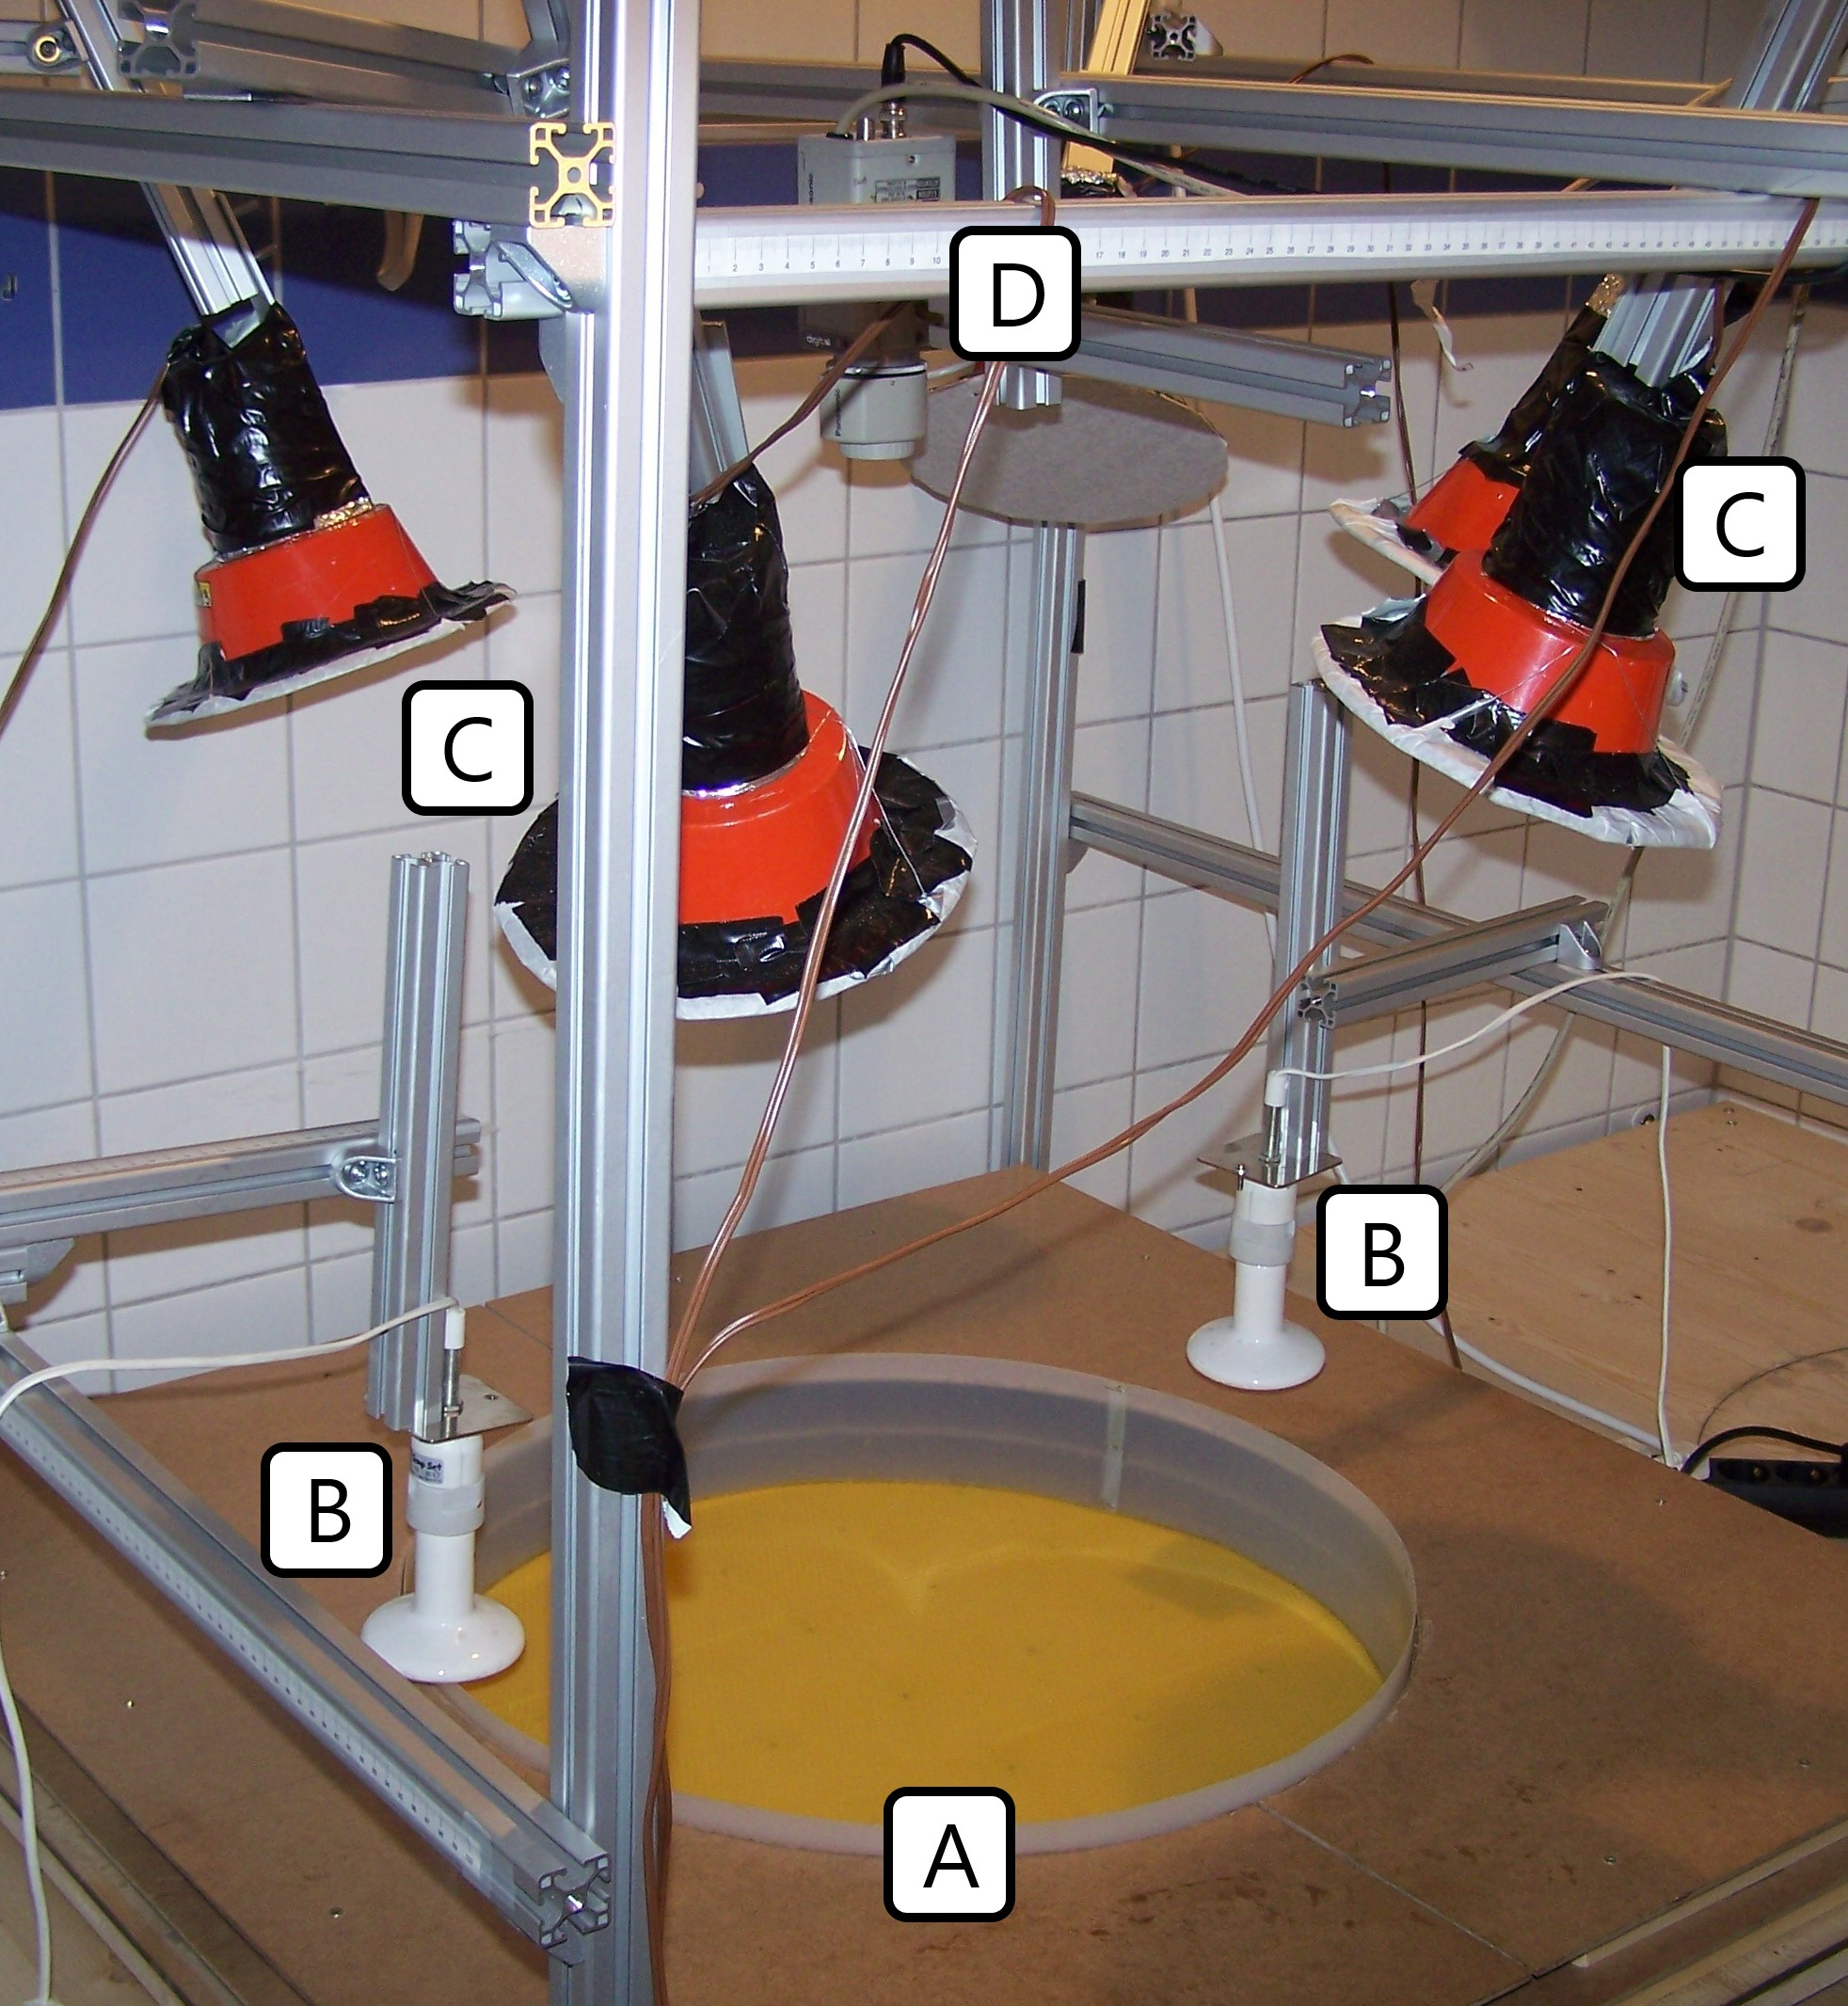
\includegraphics[width=8.7cm, height=10cm]{figures/Setup.jpg}}
    \caption{Setup with: [A] the arena itself with a circular boundary and the temperature sensors ordered in a grid with grid distance d=10cm; [B] the heating elements one on the left above the optimum, and another one on the right above the sub-optimum; [C] lamps that produce diffused red light with a wavelength $\lambda_{0} \approx 700nm$; and [D] a FLIR infrared camera that captures the bees trajectories}
    \label{fig:Setup}
\end{figure}

\section{Experimental Runs}

Although it is known that young honeybees in laboratory experiments prefer a certain ambient temperature \cite{heran1952}, which they usually actively seek, the individual runs only rarely showed a direct uphill walk in the gradient with a subsequent resting phase at the optimal temperature of 36 \textdegree C, which was expected to be the predominant behaviour.
On the contrary it appears that they display a variety of motion trajectories, that at a first glance could be classified into four distinct behavioural types.

The four dominant types of movement, that are present in all individual bees, define the success in finding the optimal spot within the arena. These characteristic movements are often present several times in each experimental run and can be described as following:

\begin{itemize}
    \item Goal Following behaviour (\textbf{GF}): the bee moves towards the optimum with a constant velocity
    \item Immobile behaviour (\textbf{IB}): the bee has a low velocity or none at all
    \item Wall Following behaviour (\textbf{WF}): the bee moves along the boundary with a Gaussian distributed velocity
    \item Random Walking behaviour (\textbf{RW}): the bee moves randomly and with random velocities uphill and downhill through all zones 
\end{itemize}

The 16 given example trajectories in figure \ref{fig:Well_Beehaved} are instances where subjectively one of the behaviours was more prevalent than the others, four for each of the four types.
\\
However, it is necessary to mention here already, that most of the bees show a combination of those different movements, often randomly changing between them, which mostly eradicates the attempt to classify a bee purely as an uphill or random walker. Nevertheless, the collocation of the movement types and their order definitely affect the success of a bee to actually spend most of its experimental run-time within a satisfactory ambient temperature and heterogeneous swarms, where individual behaviours differ from one to another, are suspected to outperform their homogeneous counterparts. \cite{Kengyel2015} 
\begin{figure}
    \centering
    \frame{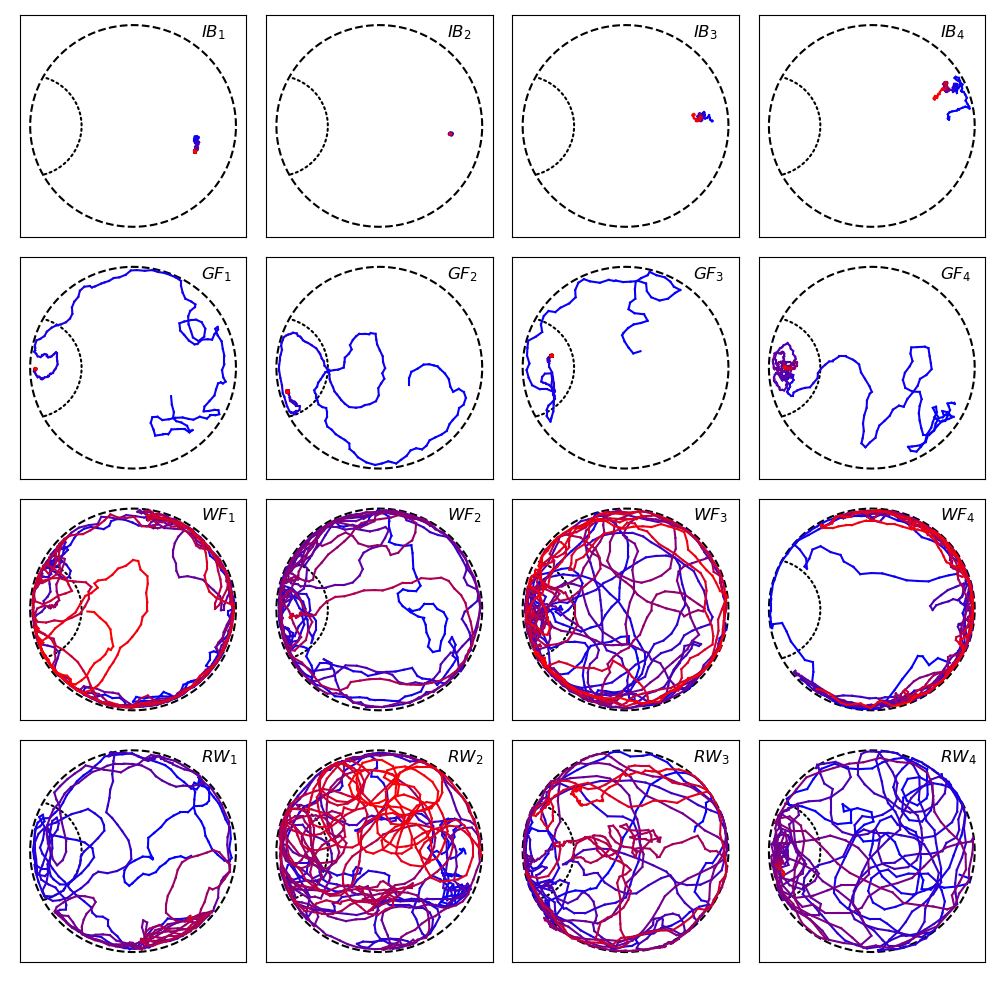
\includegraphics[width=14.7cm, height=14.7cm]{figures/Well_Beehaved.png}}
    \caption{Shown are 16 different trajectories, subjectively categorized into four different behavioural types by trained human perception. For each type (IB or immobile, GF or goal following, WF or wall following and RW or random walking behaviour) we chose four representative trajectories. Each trajectory is color coded over the whole run of the experiment, with blue being the color at the beginning of the run, gradually reaching red at the end of it. The dashed line represents the wall of the arena and the dotted line represents the warmest area (or temperature optimum) within it.}
    \label{fig:Well_Beehaved}
\end{figure}




\chapter{Methods}
\label{cha:Methods}

%As the bees have been showing a range of different types of trajectories, ranging from random seeming walks, over preferred movement in the vicinity of the walls and and almost straight uphill walks to no movement at all and often a mixture of those types a system to describe them all was developed. In molecular chemistry and molecular biology 

\begin{table}[H]
\caption{Description of the used variables in order of appearance}
    \centering
    \begin{tabular}{p{1.4cm}|p{12.4cm}}
         \textbf{Variable} & \textbf{Description} \\
         \hline
         \hline
         $m_{i}$ & inertial mass of a particle  \\
         \hline
         $\vec{x_{i}}$ & position of a particle   \\
         \hline
         $\gamma$ & friction coefficient  \\
         \hline
         $t$, $t'$ & time domain of the real time \\
         \hline
         $v_{0}$ & driving velocity of a particle/bee\\
         \hline
         $\hat{n}_{i}$ & orientation of a bee \\
         \hline
         $V$ & temperature gradient \\
         \hline
         $D$ & Diffusion coefficient \\
         \hline
         $\eta$ & Gaussian distributed white noise \\
         \hline
         $\delta$ & Dirac delta function \\
         \hline
         $\theta$ & turning angle \\
         \hline
         $a_{\theta}, a_{v}$ & coupling coefficient for the set of the embedded Langevin equations \\
         \hline
         $\langle r^{2}(\tau) \rangle$ & general mean squared displacement MSD\\
         \hline
         $\tau$ & time domain of the general mean squared displacement from within $T$\\
         \hline
         $\langle r^{2}(\tilde{t}) \rangle$ & time-averaged squared displacement TMSD\\
         \hline
         $\tilde{t}$ & time domain of the time-averaged mean squared displacement from within $\tilde{T}$ \\
         \hline
         $\langle r_{M}^{2}(t) \rangle$ & segmented mean squared displacement SMSD of a single branch $m$ from a set of branches $M$ \\
         \hline
         $S_{\theta}, S_{v}, S_{RT}$ & power spectrum of angle $\theta$, velocity $v$ and the random telegraph noise\\
         \hline
         $\omega$ & frequency within the frequency domain \\
         \hline
         $t_{s}, t_{w}$ & mean sitting and walking duration \\
         \hline
         $\Delta T$ & difference in local temperature and global optimum \\
         \hline
         $\alpha$ & exponent of the different power laws / anomaly parameter \\
         \hline
         $C_1, C_2, C_3$ & polynomial constants \\
         \hline
         $K_{\alpha}$ & ``generalized'' diffusion coefficient \\
         \hline
         $D_{\alpha}$ & time dependent diffusion coefficient \\
         
    \end{tabular}
    \label{tab:vardescription}
\end{table}
\newpage


\section{The Langevin Equation}

\subsection{General Formulation for the Position $\vec{x}(t)$ }

The spatial movement of non-equilibrium state systems, to which the bees, and in fact all other animals belong, are usually described by the theory of Brownian motion. To analyse a system in a physical manner that covers different types of movements we try to draw parallels between the self propelled bees and inanimate particles that are guided by active transport in the presence of some attractive or repulsive potential.
\\
The Langevin equation is hereby the fundamental equation to describe a trajectory of an object in space. In the present case, it is sensible to settle for the two-dimensional formulation, as the trajectories are confined to a circular plane. The equation treats the macroscopic movement in dependence of the microscopic and stochastic fluctuations of its surroundings and is formulated as:

%\begin{equation}
%   \underbrace{m_{i}\frac{d^{2} \vec{x_{i}}}{d t^{2}}}_\text{inertia} = - \underbrace{\gamma\frac{d \vec{x}_{i}}{d t}}_\text{friction} + \underbrace{\gamma v_{0} \hat{n}_{i}}_\text{propulsion} - \underbrace{\nabla V}_\text{drift} + \underbrace{\sqrt{2 D \gamma^{2}}\eta}_\text{noise}
%\end{equation}

\begin{equation}
\label{eq:Langevin_base}
    m_{i}\frac{d^{2} \vec{x_{i}}}{d t^{2}} = -\gamma\frac{d \vec{x}_{i}}{d t} + \gamma v_{0} \hat{n}_{i} - \nabla V + \sqrt{2 D_{x} \gamma^{2}}\eta
\end{equation}

%\hspace{2.9cm}\emph{inertia}\hspace{0.7cm}\emph{friction}

with $\eta$ being uncorrelated Gaussian white noise. Its auto-correlation function results in a $\delta$-function for two points in time $(t)$ and $(t')$ as
%, resulting its graph to be zero everywhere except at zero itself $(t-t')|t=t'$ as

\begin{equation}
\label{eq:Noise_corr}
    \langle \eta(t), \eta(t') \rangle = \delta(t-t')
\end{equation}

%The first term in equation \ref{eq:Langevin_base} describes the inertial movement of a particle, but as it contains a variable for a kind of mass that is not present in this system, the mass can be set to $m_{i}=1$.
The first term in equation \ref{eq:Langevin_base} describes the inertial movement of a particle, but as a bee firstly is self propelled and secondly has a negligible inertial mass of a tenth of a gram, this term as a whole can be neglected.
\\
The second term represents the dissipation this particle is experiencing, depending on a friction coefficient $\gamma$.
\\
The term $\gamma v_{0} \hat{n}_{i}$ is the particles propulsion in the direction of its orientation, and $\nabla V$ signifies the drift of the particle in presence of a gradient.
\\
The last term portrays the noise that is acting on a particle, usually caused by thermal movement of the surrounding particles.
\\
In the case of a bee this noise encloses (external and) mainly inherently present fluctuations, which can not be measured in an experiment in a sufficient way. In this context $\eta$ is a stationary and ergodic Gaussian white noise with zero mean (see \ref{eq:Noise_corr}).
\\
At this step we can draw $\gamma$ out and extended the drift by a coefficient $1/\gamma$, coupling solely the gradient to the friction coefficient.
\\
This leads to a reduced Langevin equation that is fitted specifically for the systems needs:

\begin{equation}
\label{eq:Langevin_reduce}
\boxed{
    \frac{d \vec{x_{i}}}{d t} = v_{0} \hat{n}_{i} - \frac{1}{\gamma} \nabla V + \sqrt{2 D_{x}}\eta
    }
\end{equation}

with

\begin{equation}
\label{eq:vector_n}
    \hat{n}_{i} = \frac{d\vec{x}_{i}}{dt} \left|\frac{d\vec{x}_{i}}{dt}\right|^{-1} = 
    \begin{bmatrix}
    cos\theta \\ sin\theta
    \end{bmatrix}
\end{equation}


\subsection{Custom Model for the Orientation $\hat{n}(t)$}

It should be mentioned that the equation is still tailored to represent a particle in 2 dimensions which has two degrees of freedom for its translation and therefore the noise term can act on it, resulting in a sideways or backwards movement. This is not really possible in the case of a bee as it is assumed that it always moves head first and therefore has an axis of orientation.
Though in this case it makes sense to introduce another Langevin equation to the angle of the normal direction $\hat{n}_{i}$, thereby creating a set of coupled differential equations and formulate it as following:

\begin{equation}
\label{eq:Langevin_theta}
    \frac{d \theta}{dt} = - f(\theta, V) + \sqrt{2D_{\theta}}\eta_{\theta}(t)
\end{equation}

again with $\eta_{\theta}(t)$ acting uncorrelated in time

\begin{equation}
\label{eq:noise_theta}
    \langle \eta_{\theta}(t), \eta_{\theta}(t') \rangle = \delta_{\theta} (t - t')
\end{equation}

A first assumption that can be made here is that the bees reorient depending on the gradient direction which we can linearly approximate as:

\begin{equation}
\label{eq:angle_approx}
    f(\theta, V) = a_{\theta} (\theta - \theta_{0}(V))
\end{equation}

\subsection{Custom Models for the Velocity $v_{0}(t)$}

\subsubsection{Coupled Langevin Equations}

The speed of movement can be treated in a similar way by assuming that each bee generally moves with a characteristic base velocity $v_{bee}$ that again is only modified through the application of Gaussian distributed noise. The assumption that the gradient has an influence on the movement holds true regarding the velocity as well. Therefore we formulate yet another Langevin equation for the velocity $v_{0}(t)$:

\begin{equation}
    \frac{dv_{0}}{dt} = - a_{v} (v_{0} - v_{bee}(V)) + \sqrt{2D_{v}}\eta_{v}(t)
\end{equation}

with

\begin{equation}
\label{eq:Langevin_vel}
    \langle \eta_{v}(t), \eta_{v}(t') \rangle = \delta_{v}(t - t')
\end{equation}

\subsubsection{Random Telegraph Signals $RTS$}

Looking at the experimental data and at how the bees move and stop at seemingly random intervals, suggests yet another approach for the analysis. The assumption is that the velocities of the bees basically switch between these two values $v_{bee}$, the velocity at times where they walk with an individual characteristic speed and $v = 0$ at times where they do not walk at all. 
%Those two velocities are expected to be the two means of a bimodal amplitude distribution with an individual shape for each experimental run. 
Those two velocities are expected to follow a bi-modal amplitude distribution, where the shape of each mode can be represented by a Poisson distribution.  
To describe the switching behaviour between those values we can borrow a concept that is usually used to describe a type of noise that occurs in electronic devices \cite{Machlup1954} \cite{Puglisi2016} called ``bi-stable'' or ``random telegraph signal'' (RTS) noise. The sudden jumps between two discrete values that happen at random time intervals can mathematically be formulated and modeled through a so called ``telegraph process''. 

\begin{figure}[H]
    \centering
        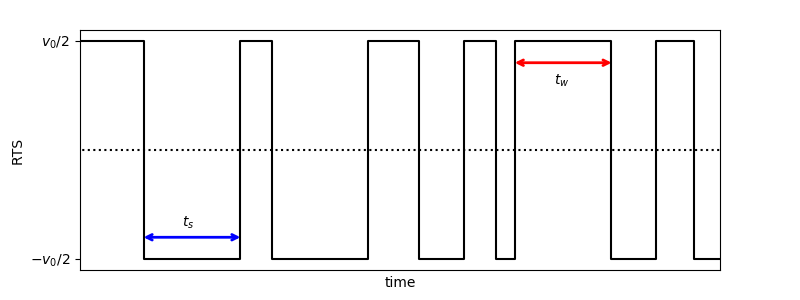
\includegraphics[width=12cm, height=5cm]{figures/2021_12_02_RTS_schematic_RTS.png}
    \caption{Schematic of a random telegraph signal with only two distinct values ($\pm v/2$) the signal can produce. The transition times $t_{s}$ and $t_{w}$ are hereby the times the system stays in either of the two states.}
    \label{fig:RTS_schematic}
\end{figure}


Previous work has shown that the noise in semiconductors can be attributed to trapping and releasing events of electrical charge carriers, which in turn cause random telegraph signals.  \cite{Guerrero2010} \cite{Leyris2006} \cite{Xiong2007} \cite{Machlup1954}
The power spectrum of the random switching between the logical ``0'' and ``1'' of these processes in general follows a decrease of $1/\omega^{2}$ \cite{Milstein2009} \cite{Puglisi2016}, but depends on the nature of the transition times, i.e. whether their mean is constant or not \cite{Machlup1954}.
In our instance the same is the case: the transition between two values, $v = 0$ and $v = v_{bee}$, is governed by two independent and stationary Poisson processes $P(m, \tau)$ with average transition timescales $t_{s}$ for when the bee is switching from walking to sitting and $t_{w}$ for when it changes from sitting to walking. 

\section{The Mean Squared Displacement}
\label{sec:MSD}

To determine the diffusion coefficient $D$ in equation \ref{eq:Langevin_reduce} a common method that can be used to analyse a particles trajectory is the mean squared displacement ($MSD$), which is a measure for the particles deviation from an initial reference position.
The $MSD$ is characterized as an average ensemble for the trajectories $\vec{X}_n$ of numerous particles $N$ after a time period $\tau$.

\begin{equation}
\label{eq:MSD_sum}
    MSD(\tau)\equiv\langle x^2(\tau)\rangle:=\lim\limits_{N\rightarrow\infty}\frac{1}{N}\cdot\sum\limits_{n=1}^N\left(\vec{X}_n(\tau)-\vec{X}_n(0)\right)^2  
\end{equation}

The value for $\tau$ in equation \ref{eq:MSD_sum} is equivalent to the duration of the experiments described in chapter \ref{chap:experiments} and we expect behaviour that is on average directly proportional to a power law $\tau^{\alpha}$. If $\alpha = 1$ we have a linear relationship between the MSD and $\tau$ that classifies the observed trajectories as normal diffusive, which indicates \cite{Lindner2008} little to no noise acting on the movement. For the cases with stronger noise, the $MSD$ implies saturating and sub-diffusive behaviour with $\alpha < 1$ and linearly growing and super-diffusive behaviour with $\alpha > 1$.

\begin{figure}
    \centering
    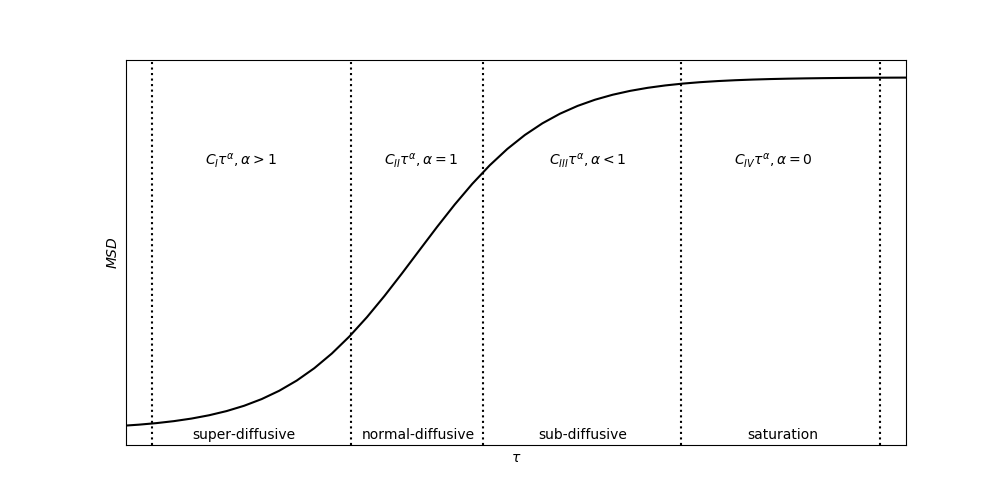
\includegraphics[width=14cm, height=7cm]{figures/2021_12_02_RTS_schematic_MSD.png}
    \caption{Schematic of a mean squared displacement over a given time domain. The progression shows a power law $\tau^{\alpha}$ first with $\alpha > 1$, continuing with a linear increase where $\alpha \approx 1$ and a saturating section where $\alpha \ll 1$, which ends in a plateau and $\alpha=0$. The different types of functions of these zones describe different grades of diffusivity.}
    \label{fig:MSD_schematic}
\end{figure}

If a statement needs to be made about the individual experimental runs, hence individual particles $N$, the $MSD$ can be redefined through a time average of a single trajectory $\vec{X}(t)$ as

\begin{equation}
\label{eq:MSD_int}
    TMSD(\tau) \equiv \langle x^2(\tilde{t})\rangle:=\lim\limits_{\tilde{T}\rightarrow\infty}\frac{1}{\tilde{T}}\cdot\int\limits_0^{\tilde{T}}\left(\vec{X}(t+\tilde{t})-\vec{X}(t)\right)^2\;\mathrm{d}t
\end{equation}

which delivers a measure for how much a particle has been displaced between times $t$ and $t+\tilde{t}$ for all possible $\tilde{t}$ within the duration $\tilde{T}$.

Another possibility to look at the data has a different and rather numerical approach, introducing the concept of a boundary to the system, where the coordinates of every collision with the arenas walls are treated as a new starting point $t_{0}$ for the $MSD$ and then averaged over the whole family of resulting curves $M$.

\begin{equation}
\label{eq:MSD_coll}
    SMSD(\tau) \equiv \langle x^{2}_M(t) \rangle := \frac{1}{M}\cdot\sum\limits_{m=1}^M|\vec{x}_m(t) - \vec{x}_m(t_{0})|^{2}
\end{equation}

The expectation that the results will indicate a behaviour ranging from sub- to super-diffusive holds true for equations \ref{eq:MSD_int} and \ref{eq:MSD_coll} as well.

\section{$1 / \omega^{2}$ Noise and the Power Spectral Density}
\label{sec:PSD}

%In time series analysis it is useful to look for recurring patterns in the data points and the power spectrum or power spectral density (PSD) is on that account an practical way to find the frequency components the data consists of.
%[TODO sentence]The Wiener-Khinchin theorem [TODO Cite Wiener 1930, Khinchin 1934] states that the autocorrelation function of a stationary random process has a spectral configuration that is given by the power spectrum of that process.
%But useful information can be extracted even if the signal is indicating that white noise is the dominating influence by analysing the power spectrum behaviour over a range of 
In time series analysis it is common to investigate a non-periodic signal in regard of its noise ratio. To do that, one can look at its spectral content via the power spectral density (PSD). It is represented as the power per unit of bandwidth of the frequency domain of a given time series. Thereby different slopes of the PSD indicate different processes and types of noise, describing in this instance different types of bee behaviour. 
White or thermal noise is characterised by a flat spectral density, meaning that it shows that same intensity, or amplitude over the whole range of the frequency domain. Brownian noise, or noise that drops proportional to $1/\omega_{2}$ can be an indicator for Brownian motion, and $1/\omega$ can have a multitude of different reasons \cite{Milotti1995}. It is well understood inside a context of transported electrons in electronic devices or dynamics within biophysics \cite{Dewey1992} \cite{Clay1976}, and will be further discussed in section \ref{sec:RTS}.

\begin{figure}[H]
    \centering
    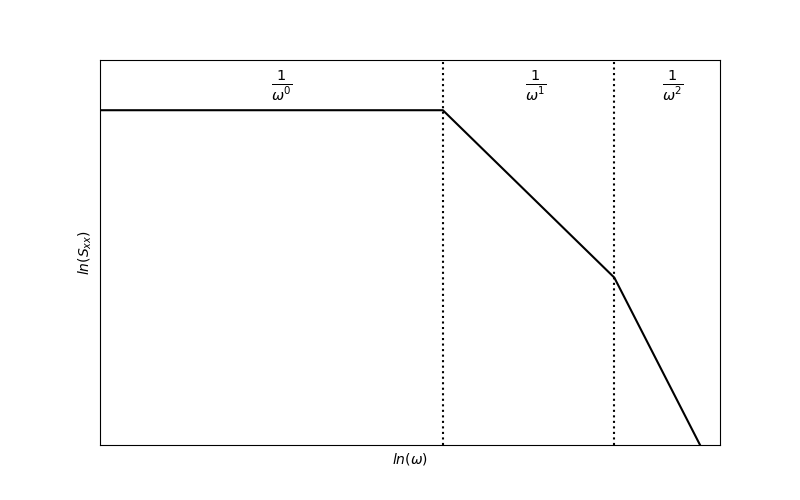
\includegraphics[width=14cm, height=8cm]{figures/2021_12_02_RTS_schematic_PSD.png}
    \captionsetup{width=12cm}
    \caption{Schematic of a power spectral density with an amplitude of a frequency range. Usually displayed in double logarithmic plots. The rate of change of the amplitude are an indicator for different kinds of noise that act on a system. The amplitude thereby follows a decrease proportional to $1/\omega^{\alpha}$ with different exponents $\alpha$, which stand for different types of noise. A system that can be described by Gaussian white noise has a power spectrum that is constant. Systems with a $1/\omega$ or $1/\omega^{2}$ decrease of the PSD are common to pink noise and brown noise respectively.}
    \label{fig:PSD_schematic}
\end{figure}

The Wiener-Khinchin theorem states, that the PSD can in general be defined as the Fourier transform of the auto-correlation function of any signal $x(t)$ \cite{Wiener1930} \cite{Khintchine1934}

\begin{equation}
\label{eq:PSD_base}
    PSD \equiv S_{xx}(\omega) := \tilde{X}^{\dagger}(\omega) \cdot \tilde{X}(\omega) = |\tilde{X}(\omega)|^{2}
\end{equation}

with

\begin{equation}
\label{eq:FT}
    \tilde{X}(\omega) = \int{x(t) \cdot e^{-\imath \omega t}}dt
\end{equation}

\subsection{Power Spectral Density of $\theta(t)$}

The power spectra for the angle $\theta$ are expected to be dependent on the temperature gradient, assuming that it acts as if a little spring is attached to the bees direction, pulling it to the higher temperature and more easily into the optimum. A PSD that scales with $1/\omega^{2}$ would indicate simple Brownian motion and no dependence on the temperature, and a progression, that flattens into a $1/\omega$ scaling or saturates entirely at some point, illustrates a dependence. Noteworthy at this point is the fact, that a well potential (or a literal wall) could lead to a flattening of the PSD as well

Inserting the Langevin equation for the angle $\theta$ (Eq.:\ref{eq:Langevin_theta}) into equation \ref{eq:FT} will result in the Fourier transform 

\begin{equation}
\label{eq:Langevin_FT}
    \imath\omega\tilde{\theta}(\omega)=-a_{\theta}\left(\tilde{\theta}(\omega)-\theta_{0}\delta(\omega)\right)+\sqrt{2D_{\theta}}\tilde{\eta}(\omega)
\end{equation}

The term containing $\theta_{0}$ can be neglected by subtracting the average angle $\theta$ from the time series before Fourier transforming it, and finally after solving for $\tilde{\theta}(\omega)$ we get

\begin{equation}
\label{eq:theta_FT}
    \tilde{\theta}(\omega) = \frac{\sqrt{2\ D_{\theta}}\tilde{\eta}(\omega)}{\imath\omega+a_{\theta}}
\end{equation}

The power spectral density on a time domain $T$ is given by

\begin{equation}
\label{eq:PSD_theta}
    S_{\theta} = \frac{1}{T}\langle|\tilde{\theta}(\omega)|^{2}\rangle =\frac{1}{T}\langle\tilde{\theta^{\dagger}}(\omega)\tilde{\theta}(\omega)\rangle
\end{equation}

Inserting $\tilde{\theta}(\omega)$ from \ref{eq:theta_FT} into \ref{eq:PSD_theta} results in

\begin{equation}
    S_{\theta} = \frac{2\ D_{\theta}\langle\tilde{\eta}^{\dagger}(\omega)\tilde{\eta}(\omega)\rangle\frac{1}{T}}{(\imath\omega+a_{\theta})(-\imath\omega+a_{\theta})}
\end{equation}

with the noise term $\langle\tilde{\eta}^{\dagger}(\omega)\tilde{\eta}(\omega)\rangle\frac{1}{T}$ being equal to $1$ (see equation \ref{eq:noise_theta}. This results in a power spectrum that gets its shape over the frequency domain $\omega$ through the two values of $D_{\theta}$ and $a_{\theta}$ and scaling with $1/\omega^{2}$.

\begin{equation}
    S_{\theta} = \frac{2D_{\theta}}{\omega^{2}+a_{\theta}^{2}}
\end{equation}

For low $\omega$ we expect a behaviour dominated by $2\ D_{\theta}/a_{\theta}^{2}$, for high $\omega$ we will see a drop off proportional to $1/\omega^{2}$. Acquiring the values for the two factors $D_{\theta}$ and $a_{\theta}$ can then be done through the comparison with the experimental data.

\subsection{Power Spectral Density of $v_{0}(t)$}

The same can be done for the velocity analogously, defining its PSD as 

\begin{equation}
\label{eq:PSD_velocity}
    S_{v}(\omega) = \frac{2D_{v}}{\omega^{2}+a_{v}^{2}}
\end{equation}

\subsection{Power Spectral Density of a Random Telegraph Signal}
\label{sec:RTS}

We begin by moving the telegraph signal by a constant factor of $v_{bee}/2$ and calculating the autocovariance of the signal, considering all the even and uneven transition probabilities as

\begin{equation}
\label{eq:Corr_vivj}
    C_{v_{i,j}}(t)=\sum\limits_{i}\sum\limits_{j}v_{i}v_{j}P\Big(v(s)=v_{i}\Big)P\Big(v(s+t) = v_{j}\Big| v(s)=v_{i}\Big)
\end{equation}

and through insertion of the Poission distribution

\begin{equation}
\label{eq:Poisson}
    P(m,\tau) = \frac{(\nu \tau) ^ {m}}{m!} e^{-\nu \tau} 
\end{equation}

into \ref{eq:Corr_vivj} the autocovariance $C_{\tau}$ gets out as

\begin{equation} 
\label{eq:Covariance}
\begin{split}
C_{\tau} & = \Big(\frac{v_{0}}{2}\Big)^2 [P(0,\tau) + P(2,\tau) + \cdots ] - \Big(\frac{v_{0}}{2}\Big)^2 [P(1,\tau) + P(3,\tau) + \cdots ] \\
         & = \Big(\frac{v_{0}}{2}\Big)^2 e^{-\nu \tau} \Big[1 - \nu \tau + \frac{(\nu \tau)^2}{2} - \frac{(\nu \tau)^3}{3!} + \frac{(\nu \tau)^4}{4!} - \cdots \Big] \\
         & = \Big(\frac{v_{0}}{2}\Big)^2 e^{-2 \nu \tau}
\end{split}
\end{equation}

Inserting the result of \ref{eq:Covariance} into the Wiener-Kinchin theorem

\begin{equation}
\label{eq:Wiener_Kinchin}
    S(\tau,\omega)=2\int\limits_{0}^{\infty}C_{\tau}\cos(\omega \tau)d \tau
\end{equation}

applying two times integration by parts and defining

\begin{equation}
    2 \nu = \Big[ \frac{1}{t_{s}} +  \frac{1}{t_{w}} \Big]
\end{equation}

the power spectral density can be formulated as

\begin{equation}
\label{eq:PSD_vivj}
   \implies S_{v}(t_{s},t_{w},\omega)=\frac{2v_{bee}^{2}}{(t_{s}+t_{w})\Big(\big(\frac{1}{t_{s}}+\frac{1}{t_{w}}\big)^{2}+\omega^{2}\Big)}
\end{equation}

For a set of times $t_{w}$, $t_{s}$ that are constant, equation \ref{eq:PSD_vivj} leads to a Lorentzian shape of the power spectrum.
We can now assume that $t_{s}$ is a variable dependent on the local temperature and is following a distribution of some kind, as a sitting bee constantly reassesses if the current position is a convenient one. At the same time we expect $t_{w}$ to be less temperature dependent, if it shows any dependence at all, as the sole act of walking suggests, that whatever the local temperature is, it is not accepted as an adequate spot.
\\
Therefore defining the difference between the local and the optimal temperature as

\begin{equation}
    \Delta T = \big|T_{local} - T_{optimum}\big|
\end{equation}

allows us to add the temperature dependence, integrate over the whole span of $\Delta T$ and rewrite \ref{eq:PSD_vivj} as

\begin{equation}
\label{eq:PSD_RTS}
    S_{RT} \coloneqq S_{v}(\omega)=2v_{bee}^{2}\int\limits_{0}^{\Delta T_{max}}\frac{P(\Delta T)d\Delta T}{\big(t_{s}(\Delta T)+t_{w}\big)\Big(\big(\frac{1}{t_{s}(\Delta T)}+\frac{1}{t_{w}}\big)^{2}+\omega^{2}\Big)}
\end{equation}

with $P(\Delta T)$ being the probability of being at a temperature $T$ and $\Delta T_{max}$ being the maximum deviation from the optimum temperature.

We now acquired two custom models for the velocity $v(t)$ and two descriptions of the respective power spectral densities (equation \ref{eq:PSD_velocity} and \ref{eq:PSD_RTS}), which we will compare to the experimental results. 

%\section{Computational Methods/Numerical Procedures}
%To calculate the needed values from the dataset and to fit the equations to them was done numerically by using the programming language "Python 3.6".
%The code can be found in the appendix chapter \ref{cha:Appendix}.
%\subsubsection{Calculation of $S_{\theta}$}
%The numerical procedure to calculate $S_{\theta}$ from the data arrays is to first calculate the Fourier transform using the "Fast Fourier Transformation" algorithm (FFT) on the "Discrete Fourier Transformation" (DFT) function of the angle $\theta(t)$:
%\begin{equation}
%\label{eq:DFT}
%    \tilde{\theta}_{k}=\sum\limits^{N-1}_{n=0}\theta_{n}[\cos\frac{2\pi}{N}kn-\imath\sin\frac{2\pi}{N}kn]
%\end{equation}
%where $T=N dt$ and $\omega=2\pi k$. \\
%As the FFT returns a vector in the complex plane $\mathbb{C}$, the spectral density then can be acquired through
%\begin{equation}
%    S_{\theta}(\omega) = \frac{1}{T}\left(\mathbf{Re}[\tilde{\theta}(\omega)]^2 + \mathbf{Im}[\tilde{\theta}(\omega)]^2\right)
%\end{equation}
%\subsubsection{Fast Fourier Transformation}
%\subsubsection{Fitting methods}
%\subsubsection{Box Muller Transformation}
%[table of used libraries ]
\chapter{Results}
\label{cha:Results}

The reorientation and the velocity changes lead to a trajectory ($x(t), y(t))$, which first will be characterized using the mean square displacement, before modeling $v(t)$ and $\theta(t)$ separately.

The results that are presented here are in a first step the analyzed trajectories from the in chapter \ref{Cha:Experiments} chosen 16 individuals: $IB_{1-4}$, $GF_{1-4}$, $WF_{1-4}$ and $RW_{1-4}$

\section{Segmented Mean Squared Displacement $SMSD$}
\label{sec:SMSD}

In section \ref{sec:MSD} we initially chose an approach that looks at the trajectory only in between contact with the arenas walls, in our case if the radial distance from the arenas center is greater than 29 centimeters. The $SMSD$ for each path is then calculated through equation \ref{eq:MSD_coll}.
The results are presented in a double linear plot, as it will be sufficient for the $SMSD$ whose relationship with $\tau$ is mostly linear. Although this implies that we can not extract any information about the overall diffusivity regime (super- or sub-diffusion), it is a first step to try looking at the behaviour when not biased by the boundary.
\\
We see (in figure \ref{fig:MSD_branches_BW}) that for our mostly immobile bees $IB_1$, $IB_2$, $IB_3$ and $IB_4$ the slope of the $SMSD$ lies strictly below $1$ and the segment of the trajectory we are looking at is in fact almost the whole run, as the bee rarely reaches the boundary. Looking at $IB_2$ in particular, a bee that did not move at all (see figure \ref{fig:Well_Beehaved}), we see that there is still a visible slope, or put differently, that there is still movement and diffusion, which results most likely from the noise of the tracking process.

When looking at the four exemplary bees, $GF_{1-4}$, that perform an uphill walk in the gradient, find the optimum and then stay there, we see that the process of moving shows a slope $>1$, followed by a slope $\ll 1$ for the duration that the bee spends sitting in the optimum. Looking at $GF_{1-3}$ additionally suggests that the switching between the two regimes of differing diffusivity was initiated by the contact with the boundary, as we see multiple branches of the $SMDS$ appearing, starting at zero point. $GF_4$ however never collides with the wall and therefore has a single curve which indicates strong diffusion until the optimum is reached, where once more a low valued diffusion sets in. 
\\
In the case of the bees that spend a lot of time near the boundary ($WF_{1-4}$) this definition of the mean squared displacement is not a satisfactory choice, as a big part of the experiment run gets lost through the repeated reset of the starting point. The same problem arises with the bees that show random walking behaviour ($RW_{1-4}$), but it again is apparent that there is a switching between walking with a constant velocity and resting phases.
\\


\newpage
\begin{figure}[H]
    \centering
        \frame{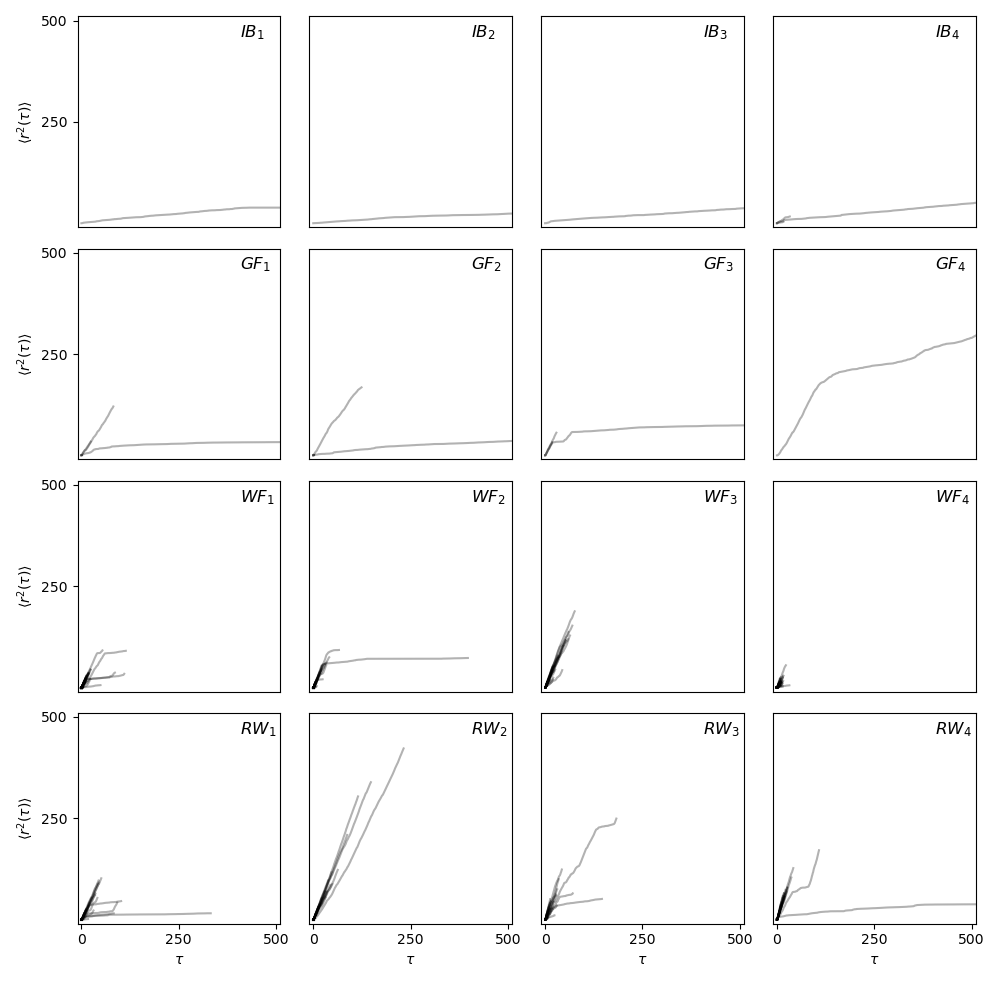
\includegraphics[width=14.7cm, height=14.7cm]{figures/MSD_branches_BW.png}}
    \caption{Depiction of the segmented $SMSD$: the resulting single branches all start at point zero, each triggered by an entry into an area that lies within a ``wall zone'', where the bees distance from the center of the arena is $r > 29$ centimeters. The opacity of each branch was reduced to 0.5 to show overlapping lines as gradations of grey. The example bees $IB_{1-4}$ show clearly and exclusively low values for the diffusion coefficient, $GF_{1-4}$ with only a few branches with a high diffusivity followed by sitting and low diffusivity. Distinction between $WF_{1-4}$ and $RW_{1-4}$ is difficult as both show numerous branches with slopes $>2$ but are showing inconsistent mixtures of high and low diffusion coefficients, where additionally big amounts of the trajectory are not taken into account.}
    \label{fig:MSD_branches_BW}
\end{figure}



\newpage
\section{Time Averaged Mean Squared Displacement $TMSD$}
\label{sec:TMSD}

Another way to look at the MSD is through a time averaged method ($TMSD$) as described in equation \ref{eq:MSD_int}.

In figure \ref{fig:MSD_lin_fit} the $TMSD$ for our 16 examples allows a first tangible analysis of the translational diffusion coefficient $D$. If we keep our initial definition of the different behaviour types, we can extract their respective values for $D$ in $n=2$ dimensions following the relation 

\begin{equation}
    \label{eq:Diff_Relation}
    TMSD \equiv \langle r^{2}(\tau) \rangle = 2nD\tau \implies m=\frac{\langle r^{2}(\tau) \rangle}{\tau}=2nD
\end{equation}

via a linear fit for $m$ and timescales $\tau$ shorter than $20$ seconds, which is the time a bee would need to traverse a distance of $60$ centimeters (i.e. the arena diameter) with a velocity of $3cm/s$. \cite{nouvian2019}

\begin{figure}%[H]
    \centering
        \frame{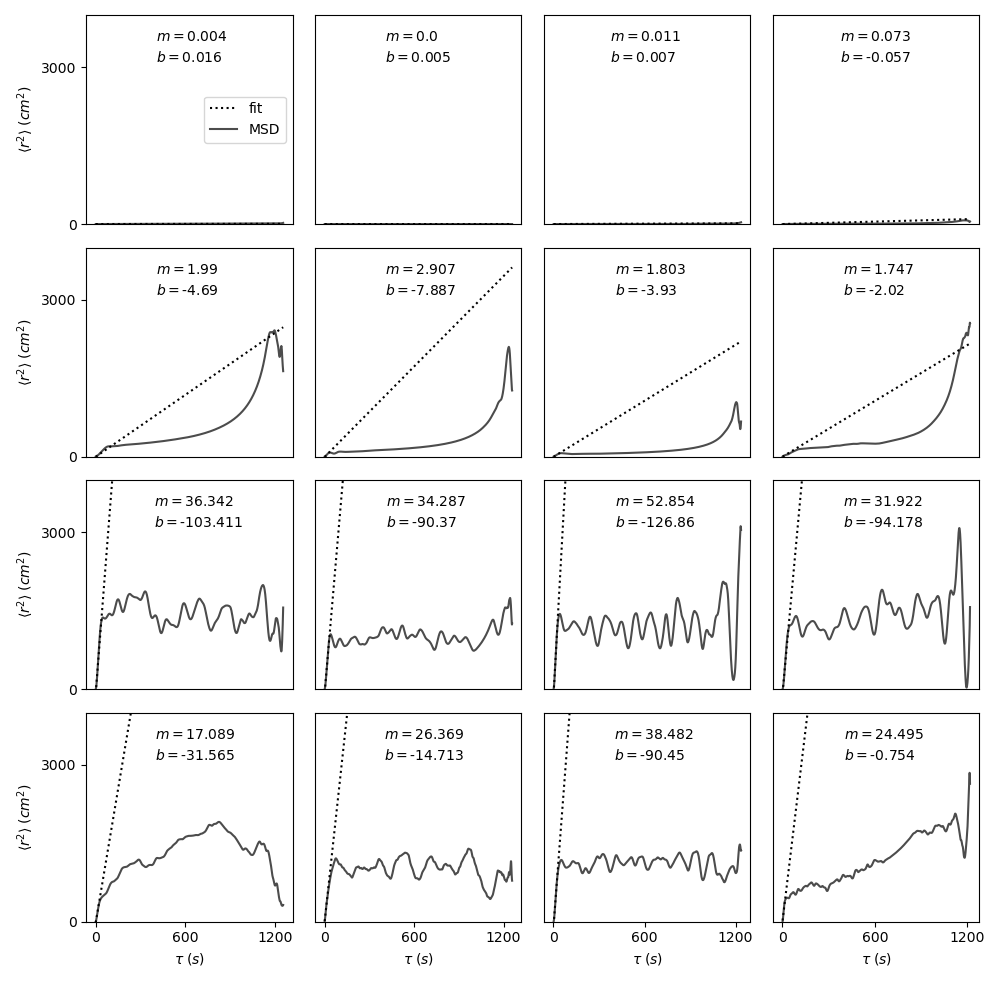
\includegraphics[width=14.7cm, height=14.7cm]{figures/lin_fit_MSD.png}}
    \caption{TSMDs of the 16 exemplary bees on a double linear scale. Only timescales $\tau < 20s$ are considered to acquire the diffusion coefficient, as this is the time a bee would theoretically need to cross the arenas diameter of $60cm$ with a velocity of $3cm/s$. The dotted line represents that linear fit for all timescales ranging in $0s<\tau<20s$. As expected the $IB_{1-4}$ show no slope at all, $GF_{1-4}$ show slopes ranging in $1.7 < m < 2.9$. $WF_{1-4}$ and $RW_{1-4}$ have slopes that are greater by a magnitude, indicating strong diffusive behaviour for short timescales at least.}
    \label{fig:MSD_lin_fit}
\end{figure}

As this diffusion coefficient flows into the noise term of equation \ref{eq:Langevin_reduce}, which affects the movement only on an infinitesimal scale $dt$, the rest ($\tau > 20s$) of the resulting MSD analysis is not of further interest in regards of the diffusion. Although noteworthy are the different slopes and forms of the MSD graphs, allowing a separation between the different types of behaviour. Immobility, represented by trajectories $IB_{1-4}$, is identified through a slope $m \approx 0.022$, and uphill movement, or trajectories $GF_{1-4}$, through a mean initial slope of $m \approx 2.112$. The distinction between $RW$ and $WF$ trajectories is again not as easily done, although $WF_{1-4}$ show oscillations in the MSD. Their slopes, although distinctly higher than with $IB_{1-4}$ or $GF_{1-4}$, have a mean value of $m \approx 38.851$ for $WF$ and $m \approx 26.609$ for $RW$ behaviour. As the slope of the $TMSD$ equals $2 n D$ with $n$ being the spatial dimensions of the tracked path, we get following values for $D$:

\begin{center}
\vspace{-2mm}
\begin{table}[H]
\caption{Translational diffusion coefficient $D$ for the different behavioural types acquired considering the slope $m$ (see figure \ref{fig:MSD_lin_fit}). The type specific diffusion coefficients only represent four bees each, the average value represents all 120 valid experiments (excluding the control sets).}
    \centering
    \begin{tabular}{p{1.2cm}|p{3.8cm}|p{4.0cm}}
         %\hline
         \textbf{Type} & \textbf{Diffusion coefficient $D$} & \textbf{Deviation $\sigma$} \\
         \hline
         \hline
         $IB_{1-4}$ & $0.006 \,cm^{2}/s$ & $\pm$ $0.030 \,cm^{2}/s$  \\
         %\hline
         $GF_{1-4}$ & $0.528 \,cm^{2}/s$ & $\pm$ $0.117 \,cm^{2}/s$  \\
         %\hline
         $WF_{1-4}$ & $9.713 \,cm^{2}/s$ & $\pm$ $2.059 \,cm^{2}/s$  \\
         %\hline
         $RW_{1-4}$ & $6.652 \,cm^{2}/s$ & $\pm$ $1.921 \,cm^{2}/s$  \\
         %\hline
         average & $2.815 \,cm^{2}/s$ & $\pm$ $3.391 \,cm^{2}/s$ \\
         %\hline
    \end{tabular}
    \label{tab:D_slope}
    \vspace{-10mm}
\end{table}
\end{center}

%\begin{center}
%    \begin{tabular}{ |p{4cm}|  }
%    \hline
%        \multicolumn{1}{|c|}{Diffusion Coefficients through slope $m$} \\
%    \hline
%        \multicolumn{1}{|c|}{$D_{IB} =0.006$} \\
%        \multicolumn{1}{|c|}{$D_{GF} = 0.528$} \\
%        \multicolumn{1}{|c|}{$D_{WF} = 9.713$} \\
%        \multicolumn{1}{|c|}{$D_{RW} = 6.652$} \\
%        \multicolumn{1}{|c|}{$D_{avg} = xx.xxx TODO$} \\
%    \hline
%    \end{tabular}
%\end{center}

\begin{figure}%[H]
    \centering
        \frame{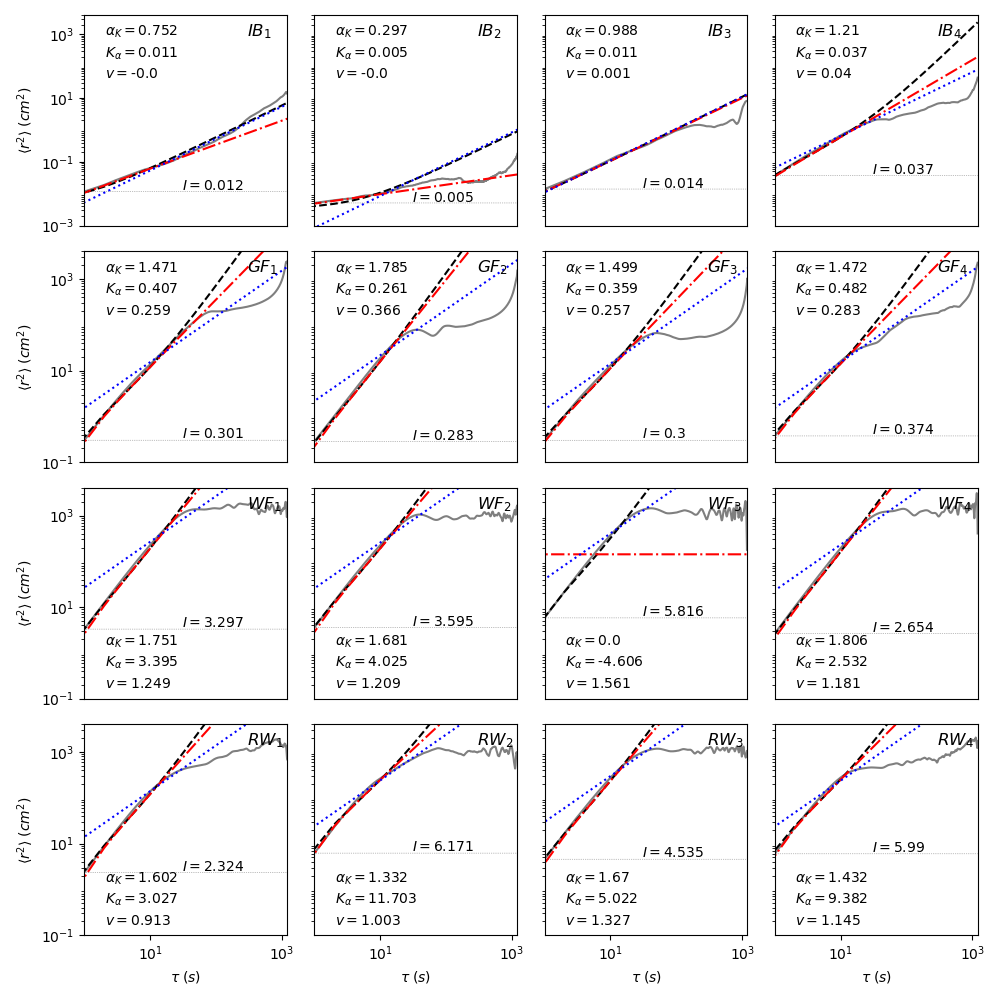
\includegraphics[width=14.7cm, height=14.7cm]{figures/2021_12_15_lin_poly_expfit_MSD_timeavg_16.png}}
    \caption{Different fits for timescales up to $20$ seconds of displacement for the 16 exemplary bees. The dotted blue line is the same linear fit that is shown in figure \ref{fig:MSD_lin_fit}. The red dash-dotted line represents a fit of a power law $\tau^{\alpha_{K}}$ to the data to show that in the logarithmic depiction a power law fits in fact better than the linear fit, showing that the diffusion taking place (if there is one at all) is a highly anomalous and super-diffusive one with $\alpha_{K}>1$ throughout all bees other than $IB_{1-4}$. The dashed black line corresponds to the quadratic term in equation \ref{eq:Diff_Relation_poly}, attempting to allow the extraction of the velocity $v$ for section \ref{sec:theta_and_velocity}. Finally, the horizontal black dotted and gently drawn line marks the intersect $I$ with the $y$-axis at $x=1$, resulting in another way to acquire the general diffusion coefficient. Additionally the values for $K_{\alpha}$ from equation \ref{eq:Diff_Relation_anomalous} are given as well.}
    \label{fig:Lin_Poly_Exp_fit}
\end{figure}

Looking at the double logarithmic plot (figure \ref{fig:Lin_Poly_Exp_fit} it is obvious that the $TMSD$ again follows a linear slope for $\tau < 10s$ and thereby implies the existence of a power law relationship up until there. This anomalous diffusive behaviour requires a different approach for the derivation of the diffusion coefficient following the relation

\begin{equation}
    \label{eq:Diff_Relation_anomalous}
    \langle r^{2}(\tau) \rangle = 2n K_{\alpha} \tau^{\alpha_{K}}
\end{equation}

where $K_{\alpha}$ is a ``generalized'' diffusion coefficient and $\alpha_{K}$ an ``anomaly parameter''. This allows for an introduction of an time dependent diffusion coefficient \cite{Metzler2000} formulated as

\begin{equation}
    \label{eq:Time_Dep_Diff_Coeff}
    D_{\alpha}(\tau) = K_{\alpha} \tau^{\alpha_{K}-1}
\end{equation}

which, put another way, introduces a ``memory'' to the system where the already elapsed trajectory has an influence on the current movement.

Although the existence of such a power law and time dependent diffusion coefficient seems to be ascertained, this approach reaches beyond the presented work and might be interesting for a separate analysis. The values for $K_{\alpha}$ are still included in figure \ref{fig:Lin_Poly_Exp_fit} and show a difference in their value, differing by an order of magnitude between $IB_{1-4}$ and $GF_{1-4}$, as well as between $GF_{1-4}$ and $WF_{1-4}$/$RW_{1-4}$. Other than that, the double logarithmic plot offers the possibility to derive the diffusion coefficient from equation \ref{eq:Diff_Relation} by locating the point of the $TMSD$ at $\tau=1$, in other words, the intersection between the $TMSD$ and the $y$-axis via the relation $I \coloneqq ln(\langle r^{2} \rangle) = ln(4D\tau)$.

%Although the existence of such a power law may be true for exemplary trajectories it must be remembered, that this can be deceiving in the end, as already small fluctuations towards the lower spectrum of the $TMSD$ can lead to a curvature of the graph, and therefore to an actually non-linear relationship. Other than that, the double logarithmic plot offers the possibility to derive the diffusion coefficient from equation \ref{eq:Diff_Relation} by locating the intersection between the $TMSD$ at $x =1$ and the $y$-axis in figure \ref{fig:Lin_Poly_Exp_fit}.

\begin{center}
\vspace{-2mm}
\begin{table}[H]
\caption{Translational diffusion coefficient $D$ for the different behavioural types acquired considering the intersect with the $y$-axis (see figure \ref{fig:Lin_Poly_Exp_fit}). The type specific diffusion coefficients represent only four bees each, the average value represents all 120 valid experiments (excluding the control sets).}
    \centering
    \begin{tabular}{p{1.2cm}|p{3.8cm}|p{4.0cm}}
         %\hline
         \textbf{Type} & \textbf{Diffusion coefficient $D$} & \textbf{Deviation $\sigma$} \\
         \hline
         \hline
         $IB_{1-4}$ & $0.017 \,cm^{2}/s$ & $\pm$ $0.012 \,cm^{2}/s$  \\
         %\hline
         $GF_{1-4}$ & $0.315 \,cm^{2}/s$ & $\pm$ $0.035 \,cm^{2}/s$  \\
         %\hline
         $WF_{1-4}$ & $3.841 \,cm^{2}/s$ & $\pm$ $1.190 \,cm^{2}/s$  \\
         %\hline
         $RW_{1-4}$ & $4.755 \,cm^{2}/s$ & $\pm$ $1.540 \,cm^{2}/s$  \\
         %\hline
         average & $1.507 \, cm^{2}/s$ & $\pm$ $1.725 \,cm^{2}/s$  \\
         %\hline
    \end{tabular}
    \label{tab:D_inter}
    \vspace{-10mm}
\end{table}
\end{center}

%\begin{center}
%    \begin{tabular}{ |p{4cm}|  }
%    \hline
%        \multicolumn{1}{|c|}{Diffusion Coefficients through intersect} \\
%    \hline
%        \multicolumn{1}{|c|}{$D_{IB} = 0.017$} \\
%        \multicolumn{1}{|c|}{$D_{GF} = 0.315$} \\
%        \multicolumn{1}{|c|}{$D_{WF} = 3.841$} \\
%        \multicolumn{1}{|c|}{$D_{RW} = 4.755$} \\
%        \multicolumn{1}{|c|}{$D_{avg} = 1.507$} \\
%    \hline
%    \end{tabular}
%\end{center}

When all the trajectories are analysed at once, the sole distribution of numerous $TMSD$ curves indicates that for short timescales $\tau < 20$ seconds the bees mostly show diffusive behaviour. The comparison of $D_{avg}$, acquired through equation \ref{eq:Diff_Relation}, and $\alpha_{K}$, which flows into equation \ref{eq:Diff_Relation_anomalous}, is illustrated in figure \ref{fig:MSD_timeavg_ALL}.

We conclude, that a diffusion coefficient $D$ which is fitted up until $\tau<20s$ is a good way to differentiate between $IB$-, $GF$- and generally random behaviour. In contrast, it is not possible to distinctly attribute a random behaviour to either the $WF$ or the $RW$ subtype.
However, bees do not move in a purely diffusive manner, even when accounting for the confinement or ballistic regime, which renders the diffusion coefficient $D$ ill defined.
A solution to that issue could be the time dependent diffusion coefficient $K_{\alpha}$ which at a first glance delivers at least the same distinction between $IB$, $GF$ and $WF/RW$. 

\begin{figure}
    \centering
    \frame{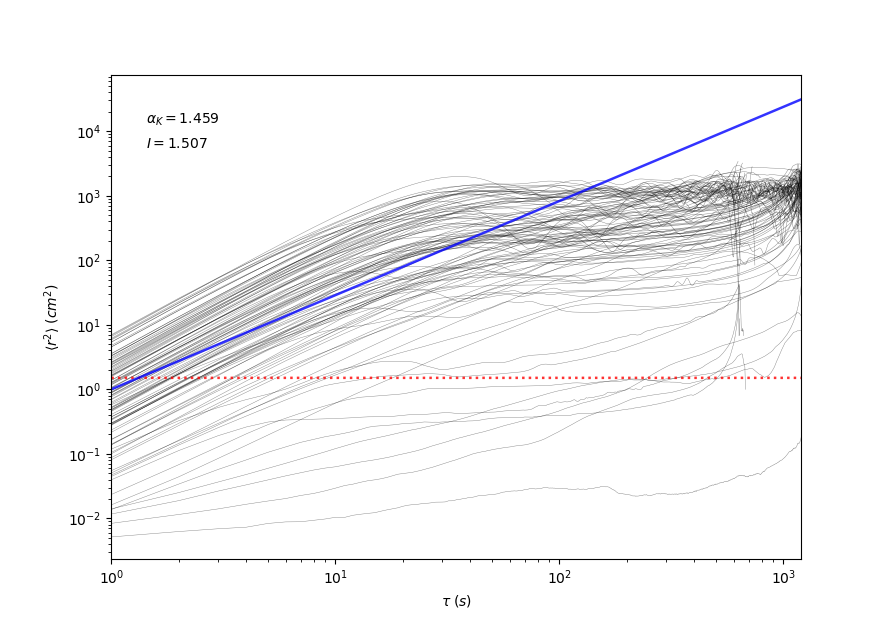
\includegraphics[width=10.7cm, height=7.66cm]{figures/2021_12_14_fit_MSD_timeavg_ALL.png}}
    \caption{Layered $TSMDs$ of all experiments with a reduced opacity in a double logarithmic plot. $\alpha_{K}$ is hereby the averaged exponent of a power law $\tau^{\alpha_{K}}$ (blue solid) and $I$ (red dotted) the average intersection with the $y$-axis at $x=0$.} 
    \label{fig:MSD_timeavg_ALL}
\end{figure}

\newpage


\section{Analysis of Angle $\theta$ and Velocity $v$}
\label{sec:theta_and_velocity}
\subsubsection{Velocities}

Revisiting equation \ref{eq:Diff_Relation} and expanding it by a quadratic term $(v \tau)^{2}$, results in a polynomial 

\begin{equation}
    \label{eq:Diff_Relation_poly}
    \langle r^{2}(\tau) \rangle = (v \tau)^2 + 2nD\tau
\end{equation}

from which we can generally derive the velocity as well (see figure \ref{fig:Lin_Poly_Exp_fit}) \cite{Tseng2002} \cite{Cherstvy2021}. Fitting the polynomial to $\tau>20s$ is hereby not resulting in any proper information, which is the reason that again only timescales of $0<\tau<20$ seconds were analysed. Hereby the initial velocities for the immobile bees $IB_{1-4}$ lie at zero centimeters per second as expected, for $GF_{1-4}$ at around $0.3cm/s$ and for $WF_{1-4}$ and $RW_{1-4}$ in a comparably wider span, ranging from $1cm/s$ to $1.5cm/s$.

\begin{center}
\vspace{-2mm}
\begin{table}[H]
\caption{Mean walking velocity for the different behavioural types acquired through the fit of the polynomial (see figure \ref{fig:Lin_Poly_Exp_fit}). The mean velocities represent four bees each.}
    \centering
    \begin{tabular}{p{1.2cm}|p{3.0cm}|p{4.0cm}}
         %\hline
         \textbf{Type} & \textbf{Mean velocity $v_{bee}$} & \textbf{Deviation $\sigma$} \\
         \hline
         \hline
         $IB_{1-4}$ & $0.010 \,cm/s$ & $\pm$ $0.017 \,cm/s$  \\
         %\hline
         $GF_{1-4}$ & $0.291 \,cm/s$ & $\pm$ $0.044 \,cm/s$  \\
         %\hline
         $WF_{1-4}$ & $1.300 \,cm/s$ & $\pm$ $0.153 \,cm/s$  \\
         %\hline
         $RW_{1-4}$ & $1.097 \,cm/s$ & $\pm$ $0.156 \,cm/s$  \\
         %\hline
    \end{tabular}
    \label{tab:vel_poly}
    \vspace{-10mm}
\end{table}
\end{center}

%\begin{center}
%    \begin{tabular}{ |p{4cm}|  }
%    \hline
%        \multicolumn{1}{|c|}{Velocities through polynomial} \\
%    \hline
%        \multicolumn{1}{|c|}{$v_{IB} = 0.010 \,cm/s$} \\
%        \multicolumn{1}{|c|}{$v_{GF} = 0.291 \,cm/s$} \\
%        \multicolumn{1}{|c|}{$v_{WF} = 1.300 \,cm/s$} \\
%        \multicolumn{1}{|c|}{$v_{RW} = 1.097 \,cm/s$} \\
%        \multicolumn{1}{|c|}{$v_{avg} = \,cm/s TODO$} \\
%    \hline
%    \end{tabular}
%\end{center}


\\
Another not quite as elegant but nevertheless better approach is to look at the histogram and thereby the distribution of the velocities of the whole run (see figure \ref{fig:Hist_velocity}) which will be needed in a following section for the analysis of the RTS as well. Compared with the results from before, this indicates some discrepancy at first sight, : the $IB_{1-4}$ have an even if small still nonzero velocity, for $GF_{1-4}$ it lies at $v \approx 1.5cm/s$, and for $WF_{1-4}$ and $RW_{1-4}$ it is well beyond $1.5 cm/s$. This can be attributed solely to the fact, that indeed the whole trajectory is considered. For $IB_{1-4}$ it suggests that this representation is more susceptible for the noise that is acting on the system, and that the bees do actually move at some point. 
%The histograms are additionally treated as two separate distributions, each normalized to $1$. The $GF_{1-4}$ behaviour indicates with its higher mean velocity, that it accelerates at some point after the initial $20$ seconds. Same holds true for $WF_{1-4}$ and $RW_{1-4}$, although their velocities at start were already high.
\\
Ignoring the velocities dependence on the temperature for now, and simply looking at the histograms, it is apparent that there indeed seems to be a switching between two (discrete) Poisson-distributed processes which can be continuously formulated as a exponential distribution

\begin{equation}
    f(x, \lambda) = \lambda e^{-\lambda x}
    \label{eq:Exponential_PDF} 
\end{equation}

for the velocities $v<0.5cm/s$ and as a Normal distribution 

\begin{equation}
\label{eq:Normal}
     f(x,\mu,\sigma) = \frac{1}{\sigma \sqrt{2\pi}} e^{-\frac {1}{2}\left(\frac {x-\mu }{\sigma }\right)^{2}}
\end{equation}

for velocities $v$ that are greater than $0.5cm/s$.
\\
The two distributions have each been separately normalized to 1 as only one of them acts on the bees velocity at a time.

\begin{figure}%[H]
    \centering
        \frame{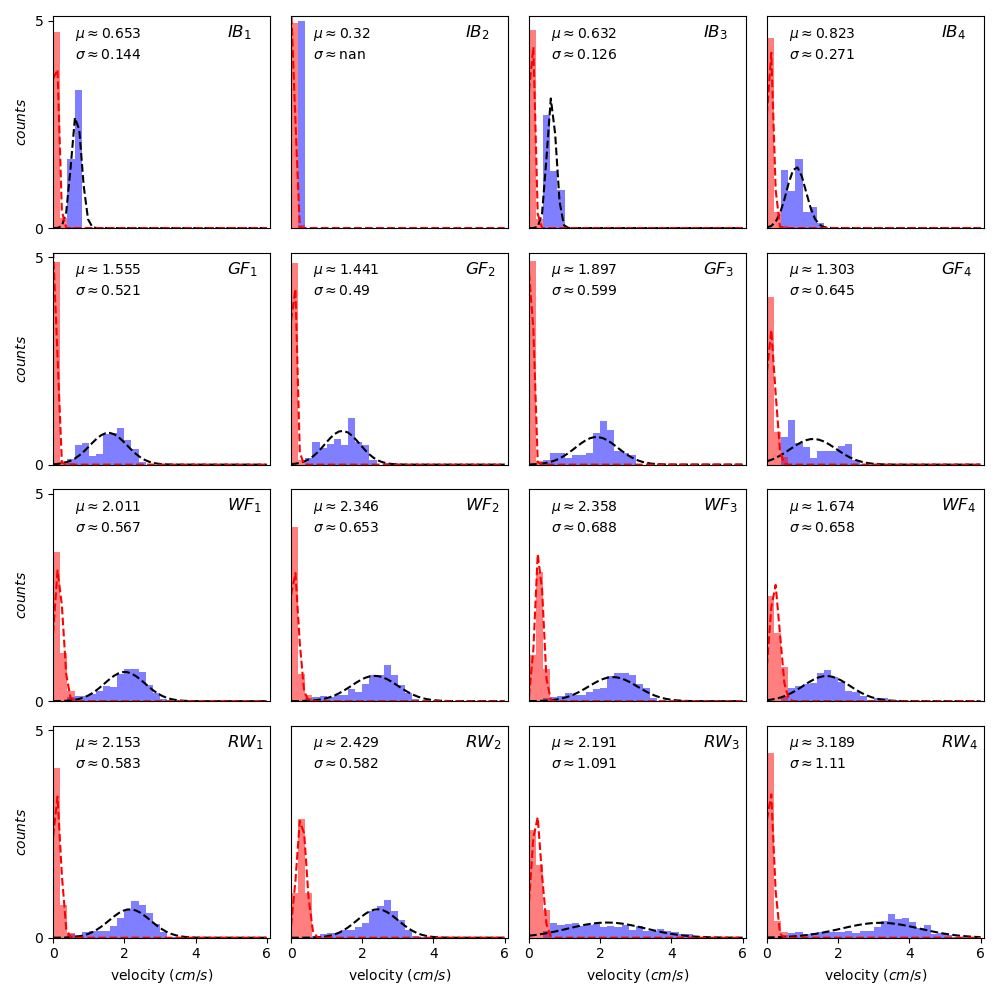
\includegraphics[width=14.7cm, height=14.7cm]{figures/Hist_velocity.png}}
    \caption{Histograms of all velocities of the 16 exemplary bees. The red bars mark all velocities $v_{bee}$ below $0.5cm/s$ for when the bee is barely moving, the blue bars depict the base velocity $v_{bee}$ greater than $0.5cm/s$, onto which a Normal distribution was fitted. The values for the mean $\mu$ and the standard deviation $\sigma$ are given for each individual run. A visible difference in velocities between the different types again allows to separate them in low ($<1cm/s$), medium ($\approx 1.5cm/s$) and high ($>2cm/s$) values.}
    \label{fig:Hist_velocity}
\end{figure}

\begin{center}
\vspace{-2mm}
\begin{table}[H]
\caption{Mean walking velocity for the different behavioural types acquired through the Gaussian fit (see figure \ref{fig:Hist_velocity}). The type specific mean velocities represent four bees each, the average value represents all 120 valid experiments (excluding the control sets).}
    \centering
    \begin{tabular}{p{1.2cm}|p{3.0cm}|p{4.0cm}}
         %\hline
         \textbf{Type} & \textbf{Mean velocity $v_{bee}$} & \textbf{Deviation $\sigma$} \\
         \hline
         \hline
         $IB_{1-4}$ & $0.607 \,cm/s$ & $\pm$ $0.018 \,cm/s$  \\
         %\hline
         $GF_{1-4}$ & $1.475 \,cm/s$ & $\pm$ $0.220 \,cm/s$  \\
         %\hline
         $WF_{1-4}$ & $2.097 \,cm/s$ & $\pm$ $0.281 \,cm/s$  \\
         %\hline
         $RW_{1-4}$ & $2.491 \,cm/s$ & $\pm$ $0.417 \,cm/s$  \\
         %\hline
         average & $1.704 \,cm/s$ & $\pm$ $0.573 \,cm/s$  \\
         %\hline
    \end{tabular}
    \label{tab:vel_gauss}
    \vspace{-10mm}
\end{table}
\end{center}

%\begin{center}
%    \begin{tabular}{ |p{4cm}|  }
%    \hline
%        \multicolumn{1}{|c|}{Velocities through normal distribution} \\
%    \hline
%        \multicolumn{1}{|c|}{$v_{IB} = 0.607 \,cm/s$} \\
%        \multicolumn{1}{|c|}{$v_{GF} = 1.475 \,cm/s$} \\
%        \multicolumn{1}{|c|}{$v_{WF} = 2.097 \,cm/s$} \\
%        \multicolumn{1}{|c|}{$v_{RW} = 2.491 \,cm/s$} \\
%        \multicolumn{1}{|c|}{$v_{avg} = TODO \,cm/s$} \\
%    \hline
%    \end{tabular}
%\end{center}

The behaviour of the velocities in presence of a gradient can as well be investigated by looking at its power spectral density $S_{v}$ over frequency domain $\omega$ (see equation \ref{eq:PSD_velocity} and figure \ref{fig:PSD_velocity}). As a flattening of the PSD and $a_{\theta} > 0$ is only recognisable in $GF_{1-4}$, this indicates that their velocities are most effectively governed by the temperature. The decrease over $1/\omega^{\alpha_{pow}}$ is present in all of them, and ranges for exponents $0<\alpha_{pow}<3$, which reveals Gaussian white noise at $\alpha_{pow}=0$ and Brownian motion at $\alpha_{pow}=2$ at high frequencies. Finally, due to the fact that most of the PSD show a decrease looking more like $1/\omega$, for which there are many explanations with the random telegraph or ``flicker'' noise from section \ref{sec:RTS} being one of them, a general dependence on the temperature can be attributed to all of the exemplary bees, excluding the immobile ones.

In conclusion it can be stated that equation \ref{eq:PSD_velocity} is a poor fit for the power spectral density $S_{v}$, meaning that $v_{0}(t)$ is not governed by noise around a characteristic mean velocity $v_{bee}$, but rather switches between velocities $v=0$ and $v_{bee}>0$.

\begin{figure}%[H]
    \centering
        \frame{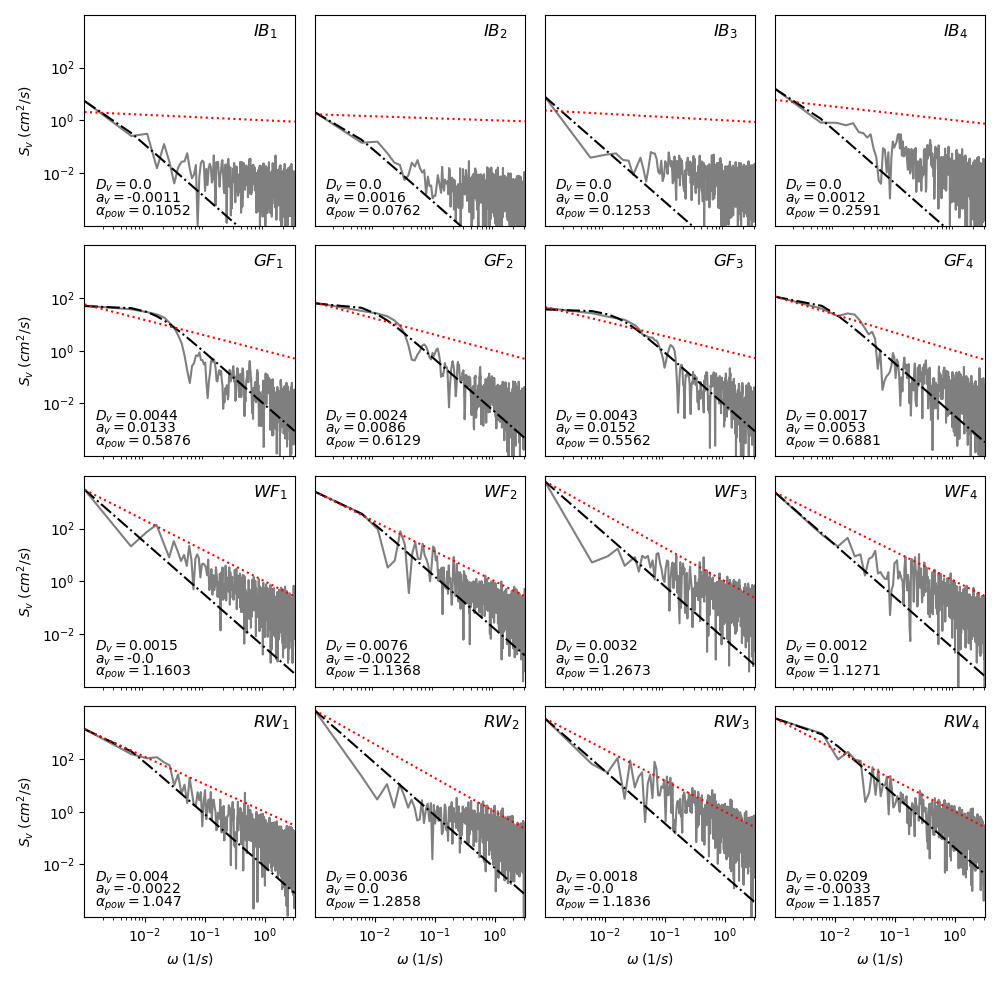
\includegraphics[width=14.7cm, height=14.7cm]{figures/PSD_velocity.png}}
    \caption{PSD of the velocity for the 16 exemplary bees, acquired through equation \ref{eq:PSD_velocity} for the dash-dotted line, representing the analytical fit for $D_{v}$ and $a_{v}$. The solid grey line depicts the PSD of the experimental data acquired through its Fourier-transformed signal. For low frequencies $\omega$ we generally see a decrease following $1/\omega^{2}$ that then switches to something more resembling a decrease proportional to $1/\omega$, meaning that first there is no influence of the temperature on the velocities followed by $\omega$ where a dependence seems possible, which may be induced by a stopping and walking behaviour. Regarding the velocities of $GF_{1-4}$ it is apparent that there is a cutoff frequency, suggesting a considerably high dependency on temperature for low $\omega$. This cutoff, even if less pronounced, is present in $WF_2$ or $RW_4$ as well, which makes sense as those particular two bees did spend a lot of time with $v=0cm/s$ in the optimum, confirming this approach in general but failing to deliver useful information for the rest of the $RW$ and $WF$ bees. What it does deliver though, is the fact that a distinction between less and more active behaviour is possible by looking at the intersect with the $y$-axis.}
    \label{fig:PSD_velocity}
\end{figure}

In the context of velocity, its general dependency on the local temperature needs to be investigated as well (see figure \ref{fig:vel_vs_dT}), as this relation is required for the drift term in equation \ref{eq:Langevin_reduce}. It is evident that the dependency is an approximately linear one, with on average higher velocities for lower temperatures and vice versa ($2.5cm/s$ at $28^{\circ}C$ and $1.0cm/s$ at $36^{\circ}C$).

\begin{figure}%[H]
    \centering
        \frame{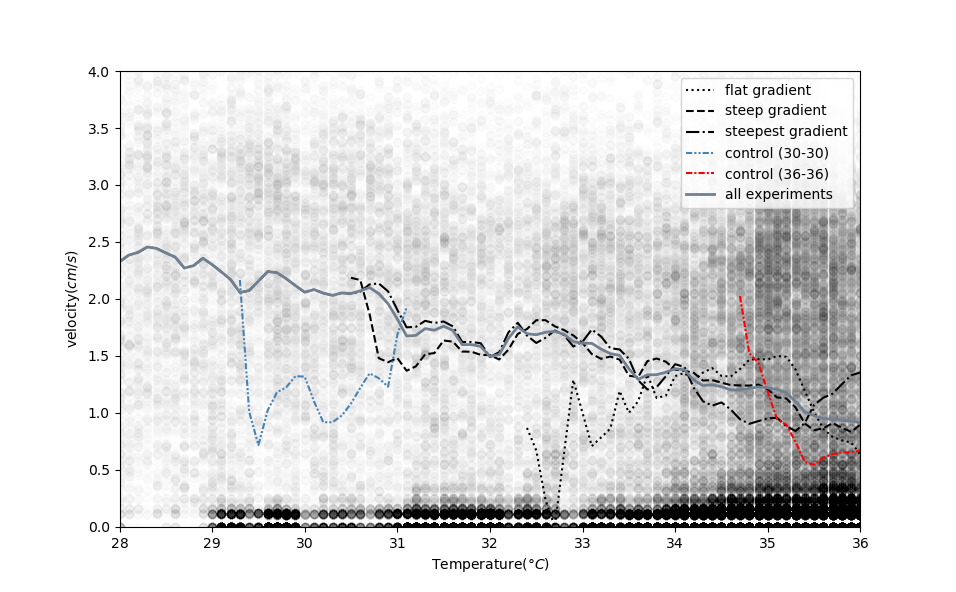
\includegraphics[width=14.7cm, height=8.7cm]{figures/2022_01_11_mean_bin_vel_vs_dT_split_grad.png}}
    \caption{Temperature dependent velocity. The background shows all velocities in all points in time of all bees. The dotted line considers only experiments with a flat gradient of around $2^{\circ}C$, the dashed line only experiments with a steeper gradient of around $4^{\circ}C$ and the dash-dotted line the steepest gradients. The solid grey line (and foundation for the linear fit) represents the mean of all experiments at all temperatures with a resolution of $0.1^{\circ}C$. The blue dash-dotted line are the control experiments, where both, optimum and sub-optimum were set to $30^{\circ}C$, similarly the red dash-dotted line consists of the corresponding control experiments at $36^{\circ}C$. The slope $b$ of the linear fit to the mean curve equals to $b=3/16$.}
    \label{fig:vel_vs_dT}
\end{figure}

\subsubsection{Turning Angle $\theta$}

To determine the values for $a_{\theta}$ and $D_{\theta}$ from equation \ref{eq:PSD_theta}, the respective PSD was modeled and fitted to the experimental data (see \ref{fig:PSD_angle}).
The fit shows a drop that is proportional $1/\omega^{2}$ for high $\omega$ in all of them, which was expected. The fact that their cutoff frequencies are randomly distributed however supports the surprising interpretation that the bees are not that thoroughly turning into the direction of highest gradient ascent. In other words, bees behave less based on the concept of ``colder'' or ``warmer than before'', but rather on ``warm enough''. %(which, as we will see, then can trigger a stopping event).

\begin{figure}%[H]
    \centering
        \frame{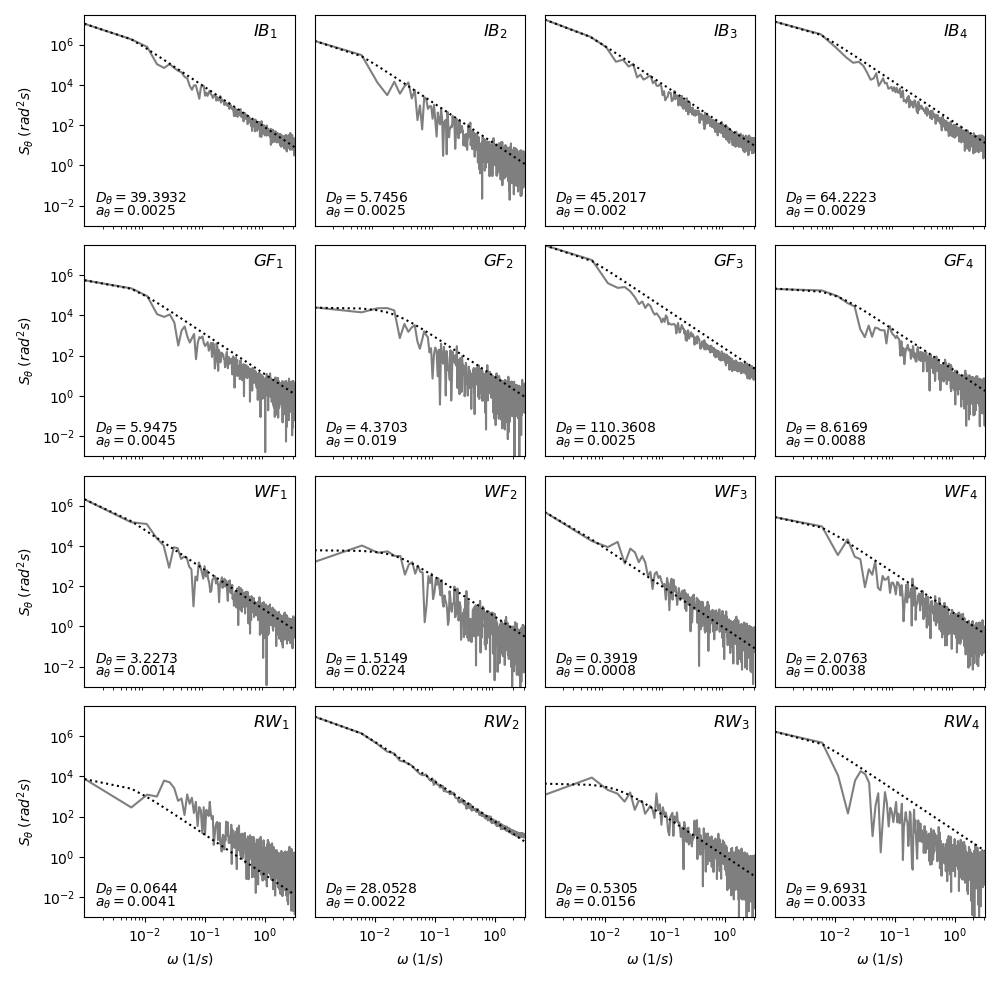
\includegraphics[width=14.7cm, height=14.7cm]{figures/2021_12_07_PSD_angle_16.png}}
    \caption{The PSDs of the angle $\theta$ for the 16 exemplary bees show interesting properties: firstly, the Lorentzian shape is practically present in every spectrum,  secondly, their cutoff frequencies are not very distinct, especially when comparing $GF_{1-4}$ with $RW_{1-4}$. In general the bees reaction to the gradient is less prevalent than expected. The different noise intensities, which can be explained by different amounts of randomness acting on the angles amplitude, are not special to any of the different behaviours. Additionally observable is, that they uniformly show a $1/\omega^{2}$ dependence.}
    \label{fig:PSD_angle}
\end{figure}

%Again looking at all the experiments at once in regarding the $D_{\theta}$ and $a_{\theta}$ pairs, we see a linear dependence between them, which seems sensible at a first glance as a bee that moves/turns a lot is more likely to find the goal (see figure \ref{fig:D_vs_a_theta}).

\begin{figure}%[H]
    \centering
        \frame{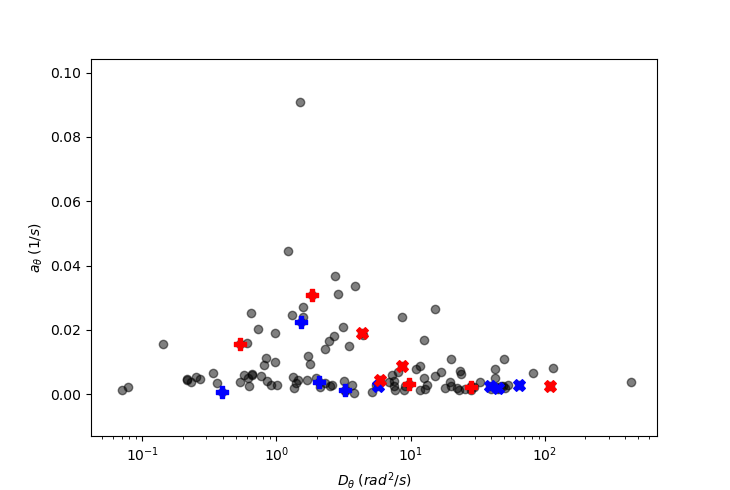
\includegraphics[width=11.5cm, height=7.5cm]{figures/2021_12_08_scatter_D_vs_a.png}}
    \caption{Values of $D_{\theta}$ plotted over $a_{\theta}$ for all bees. The red ``X'' markers stand for $IB_{1-4}$, the red ``+'' for $GF_{1-4}$, the blue ``X'' mark $WF_{1-4}$ and the blue ``+'' mark $RW_{1-4}$. The two values seem to be uncorrelated, however When looking at the plot in single logarithmic depiction ($log($x$)$), the aggregated $D_{\theta}$ over $a_{\theta}$ resemble a Log-normal distribution.}
    \label{fig:D_vs_a_theta}
\end{figure}

\newpage

\section{Analysis of the RTS}

%It was already shown, that there is an apparent switching between some type specific mean walking speed $v_{bee}$ and a velocity $v \approx 0$ (see figure \ref{fig:Hist_velocity}).

To see whether our assumptions regarding the switching behaviour between walking and stopping again follows a $1/\omega^{\alpha_{RTS}}$ decrease, and if $\alpha_{RTS}$ differs between the types, we will continue by analysing the power spectrum of the random telegraph signal as described in equation \ref{eq:PSD_RTS}.

%For that we will first try to find the average times $t_{s}$ and $t_{w}$ and their possible dependence on the temperature $T$.

For our 16 exemplary behaviour types we have already seen in figure \ref{fig:Hist_velocity} that there is a clear dominance of two uncorrelated Poisson-distributed and type specific velocities $v = v_{bee}$ and $v = 0$. To determine the mean velocity $v_{bee}$ it is sufficient to fit a continuous Gaussian distribution to the histograms velocities above $0.5 cm/s$, for as the Poisson distribution is only given for discrete values. All velocities below $0.5 \,cm/s$ are considered to be sitting as they lie just below the mean velocity for the bees that show immobile behaviour (see table \ref{tab:vel_gauss}).

%To see whether a random walking bee actually exhibits a change in velocity that can be compared to a random telegraph signal, a vivid example is given by bee $RW_3$ in figure \ref{fig:RTS_RW3}. It is evident that there is such a switching present in this particular experimental run, that actually has been chosen as an example for precisely this behaviour. 

To see whether the bees actually exhibit a change in velocity comparable to a RTS
When the definition of those two states is being plotted over the experimental run time, it indeed is observable that the resulting signal jumps randomly between ``0'' and ``1'', for $RW_{1-4}$ and $WF_{1-4}$ (see figure \ref{fig:RTS_second}) more so than for $IB_{1-4}$ and $GF_{1-4}$ (see figure \ref{fig:RTS_first}).

\begin{figure}%[H]
    \centering
        \frame{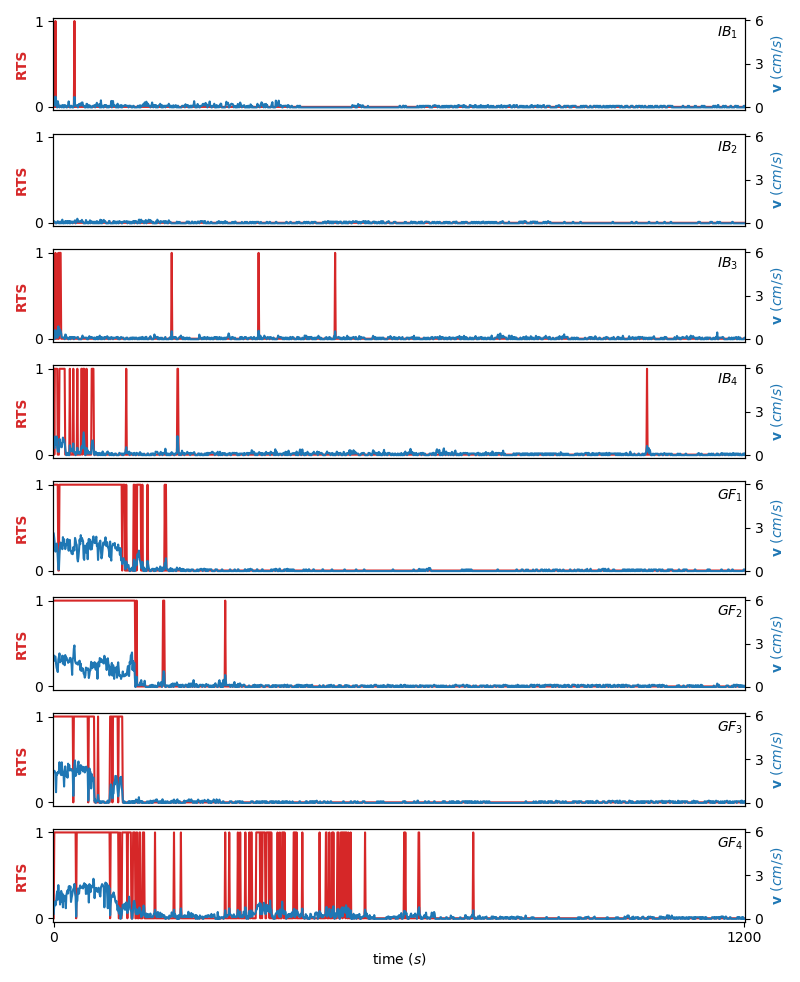
\includegraphics[width=14cm, height=18cm]{figures/2022_01_18_is_it_really_RTS_first_8.png}}
    \caption{Velocities of $IB_{1-4}$ and $GF_{1-4}$ in blue and their associated random telegraph signal in red.}
    \label{fig:RTS_first}
    \vspace{-15mm}
\end{figure}

\begin{figure}%[H]
    \centering
        \frame{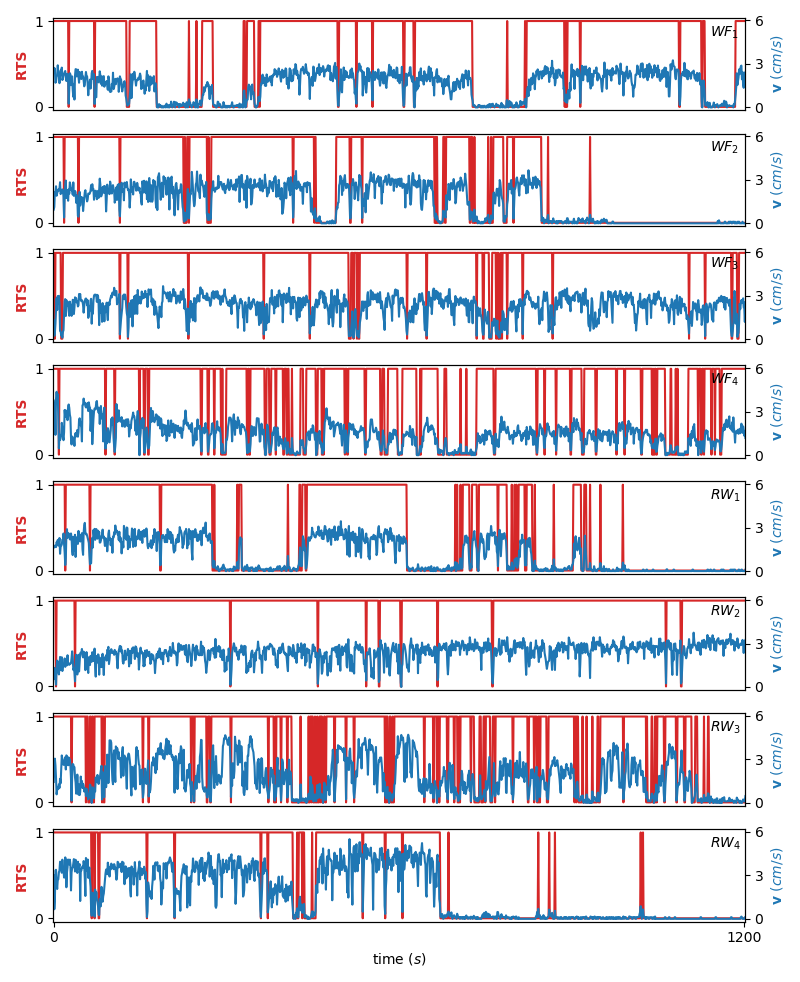
\includegraphics[width=14cm, height=18cm]{figures/2022_01_18_is_it_really_RTS_second_8.png}}
    \caption{Velocities of $WF_{1-4}$ and $RW_{1-4}$ in blue and their associated random telegraph signal in red.}
    \label{fig:RTS_second}
    \vspace{-15mm}
\end{figure}

Furthermore considering the second assumption that the duration a bee is sitting still $t_{s}$ is dependent on temperature, and the duration it walks $t_{w}$ is not, can be evaluated by looking at the correlation of $t_{s}$, $t_{w}$ and $\Delta T$ (see figure \ref{fig:ALL_stop_walk}).
$\Delta T$ is hereby the absolute difference of the local temperature $T$ at times $t_{s}$ and $t_{w}$ and the temperature at the optimum $T_{opt}$. In both cases the local temperature was defined as the mean temperature over the span of $t_{s}$ and $t_{w}$ respectively. 
Here again the recognisably different distributions indicate that the assumption holds true, the linear fit to a function $t = m \Delta T + b$ for $t_{s}$ shows a slope of $\approx -25$ whereas it is $\approx 2$ for $t_{w}$. It seems that for $t_{s}$ another function would better describe the behaviour, namely an exponential function (maybe even a power law of some sorts) and an example is given in figure \ref{fig:ALL_stop_walk} by comparing the linear fit to the fairly strong function $t = \tau \cdot e^{-\beta \Delta T}$. 

\begin{figure}%[H]
    \centering
        \frame{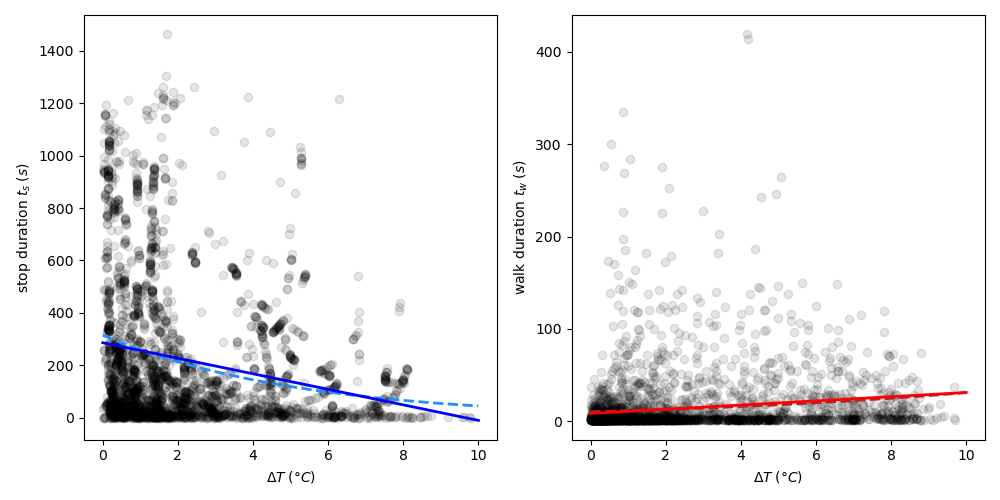
\includegraphics[width=14cm, height=6.5cm]{figures/2022_01_12_ALL_t0_t1_of_dT_scatter_nonlin_fit.png}}
    \caption{Scatter plots of the experimental stopping and walking durations $t_{s}$ (left) and $t_{w}$ (right) in dependence of the temperature $\Delta T = |T - T_{opt}|$. The blue solid line represents the linear fit, the dashed line (light blue) is a curve fit to a function $\tau \cdot e^{-\beta \Delta T}$. For higher $\Delta T$ the linear fit remains to be the better one and there seems not to be any significant improvement for lower $\Delta T$ through the exponential function. However all fits confirm what was expected: $t_{s}$ is highly temperature dependent, and $t_{w}$ is not, which is sensible, considering the fact that the $\Delta T$ for each walking duration is computed by averaging it over the span of $t_{w}$.}
    \label{fig:ALL_stop_walk}
\end{figure}

Looking at the fits of $t_{s}(\Delta T)$ for the 16 exemplary bees we see that a linear relationship would not be sufficient anymore to represent what is going on, and in this individual depiction aforementioned fit to $t = \tau \cdot e^{-\beta \Delta T}$ delivered better results (see figure \ref{fig:t_stopping_nonlin_16}) % and \ref{fig:t_stopping_nonlin_group4}).

\begin{figure}%[H]
    \centering
        \frame{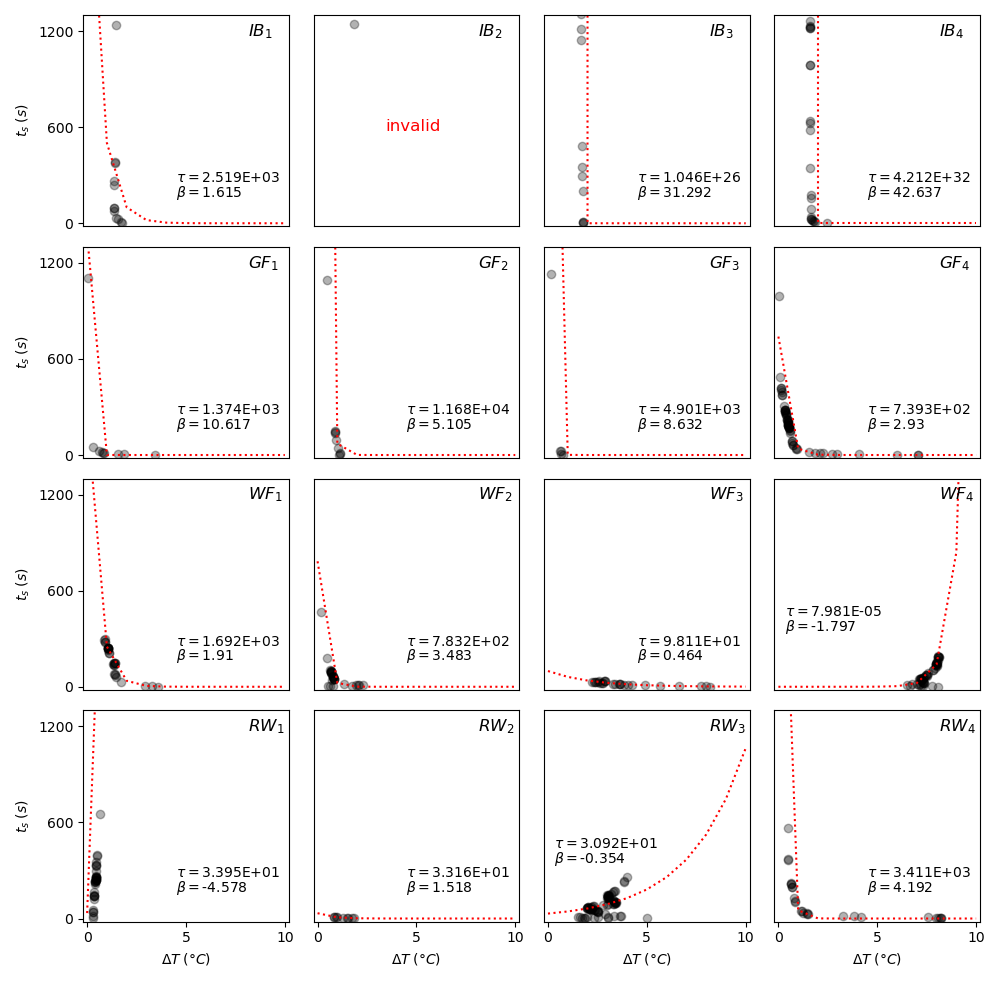
\includegraphics[width=14.7cm, height=14.7cm]{figures/2022_01_13_RTS_PSD_16_nonlin_fit.png}}
    \caption{Individual fittings for $t_{s}$ for the 16 exemplary bees. $IB_{2}$ has only a single point of data, a curve fit leads to undefined values. Note that $IB_{1-4}$ were experiments with a flat gradient of $\Delta T_{max} \approx 2^{\circ} C$, the bees have practically an infinitely high $t_{s}$ at the $\Delta T$ they have been released into the arena. $GF_{1-4}$ show low $t_{s}$ at any $\Delta T$ that is not near the optimum. $WF_{1-4}$ and $RW_{1-4}$ again are fairly random whereas there still exists a tendency towards longer stopping durations at temperatures nearer to the optimum. The red dotted line depicts the fit responding to the curve $t = \tau \cdot e^{-\beta \Delta T}$ with their individual parameters $\tau$ and $\beta$.} 
    \label{fig:t_stopping_nonlin_16}
\end{figure}

%\begin{figure}%[H]
%    \centering
%        \frame{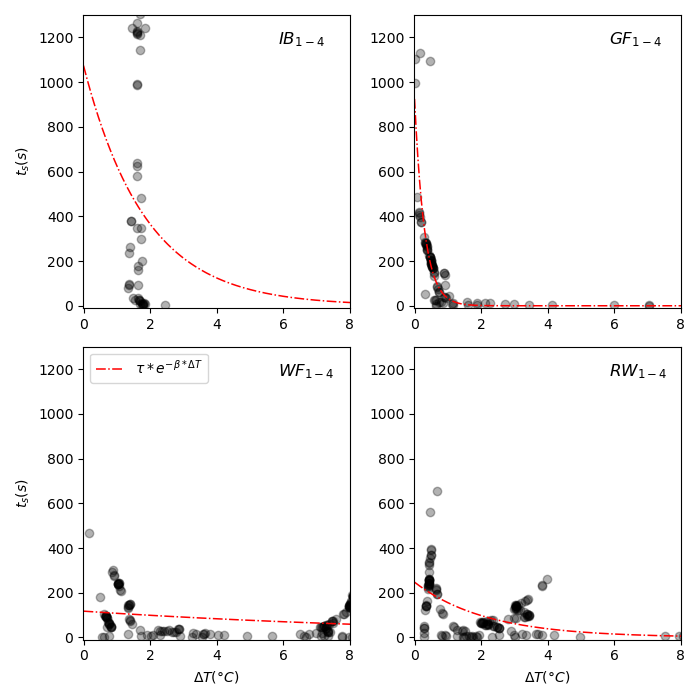
\includegraphics[width=10.7cm, height=10.7cm]{figures/2022_01_14_RTS_PSD_nonlin_fit_of_t0_group_4_V2.png}}
%    \caption{To see whether a bigger set of points leads to a clearer picture, the four individual trajectories for each type of behaviour have been grouped and $t_{s}$ is shown for each of the four types of behaviour. The red dash-dotted line depicts the fit responding to the curve $t = \tau \cdot e^{-\beta \Delta T}$ with their individual parameters $\tau$ and $\beta$. Unfortunately such a grouping is not useful in this particular case with the chosen experiments. One reason surely lies in the different gradients - the examples were initially chosen solely based on the appearance of their trajectory without other information, another one in the low number of representing experiments used. Nevertheless, the dependence is again visible and strongest in $GF_{1-4}$.} 
%    \label{fig:t_walking_nonlin_group4}
%\end{figure}

Finally, after acquiring $t_{s}$ and $t_{w}$ we can now look at the power spectra of the telegraph signals (see figure \ref{fig:RTS_PSD_16}). It is noticeable that the experimental power spectrum is only partially comparable to the analytically derived function (equation \ref{eq:PSD_vivj}). Looking at its slopes for higher $\omega$ we see that it fits best for individuals that actually experience a pronounced random telegraph signal ($WF_1$, $WF_4$, $RW_3$). In general it fits well enough for most of them, it is however partially too steep and therefore misleading: looking at $RW_2$, the fit of equation \ref{eq:PSD_vivj} suggests that there is a fairly strong switching happening, when it is known that this bee rarely sits, hence delivering not enough data points to be expressed like that. This gives rise to the questions firstly, whether there is another way of representing the switching behaviour needed, and secondly whether the data would require additional filtering.

\begin{figure}%[H]
    \centering
        \frame{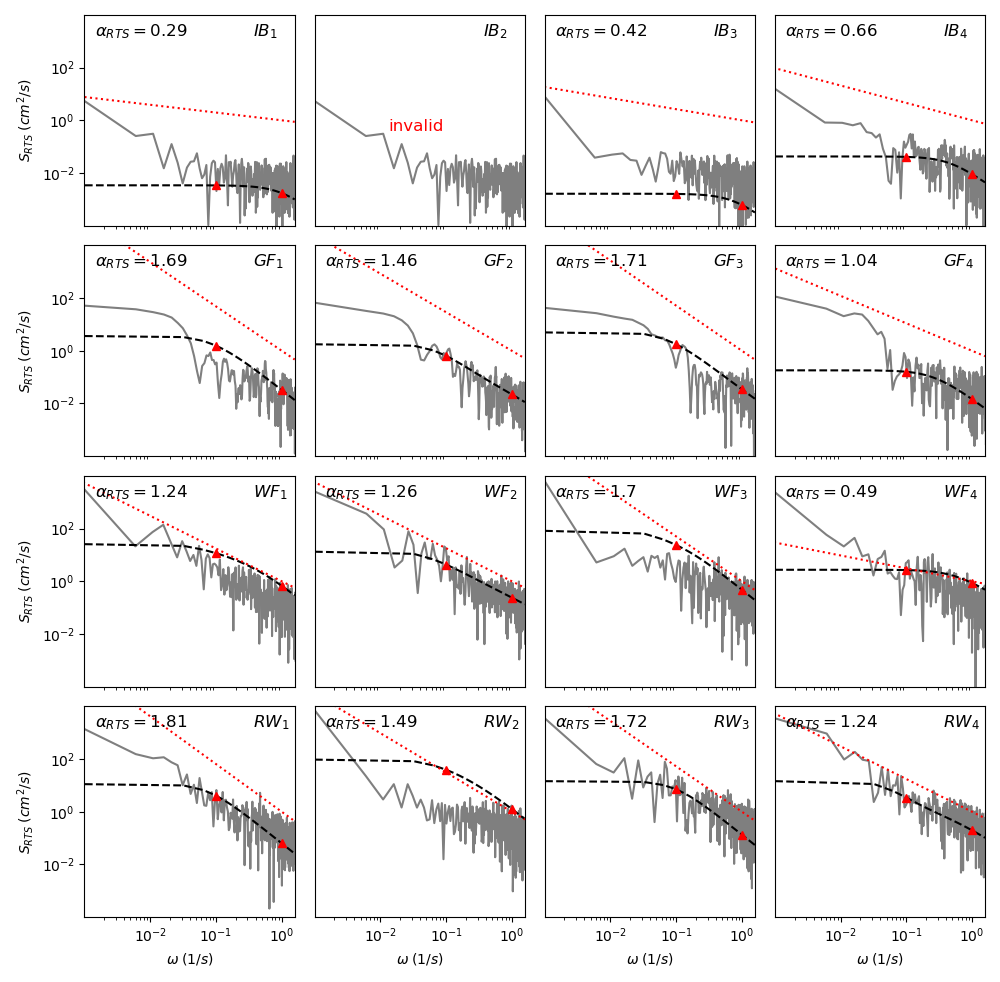
\includegraphics[width=14.7cm, height=14.7cm]{figures/2022_01_16_RTS_PSD_16.png}}
    \caption{Experimental power spectrum of the velocity (grey solid) and the analytical description of the RTSs spectrum (black dashed). The space in between the red triangles mark one order of magnitude from $10^{-1}$ to $10^0$. The red dotted line stands for a $1/\omega^{\alpha}$ relation where $\alpha_{RTS}$ is the decrease of $S_{RTS}$ over aforementioned span, given in orders of magnitude.}  
    \label{fig:RTS_PSD_16}
\end{figure}

To be able to look at all bees and all fitted values at once and see if there are similarities or patterns that let us compare them again with the subjectively and manually assigned types, everything is collectively presented in table \ref{tab:AllData}.

\begin{table}
\caption{
\textbf{ID}: experiment identification $\: |$
$\mathbf{\nabla V}$: type of gradient (1:flat, 2:steep, 3:steepest) $\: |$
\textbf{type}: manual classification $\: |$
$\mathbf{D_{TMSD}}$: see section \ref{sec:TMSD} $\: |$
$\mathbf{v_{TMSD}}$: see equation \ref{eq:Diff_Relation_poly} $\: |$
$\mathbf{K}_{\boldsymbol{\alpha}}$: time dependent diffusion coefficient $\: |$
$\boldsymbol{\alpha}_\mathbf{{K}}$: exponent corresponding to $K_{\alpha}$ $\: |$ 
$\mathbf{v_{bee}}$: mean walking velocity, see equation \ref{eq:Normal} $\: |$
$\mathbf{D_{v}}$: see equation \ref{eq:PSD_velocity} $\: |$
$\mathbf{a_{v}}$: see equation \ref{eq:PSD_velocity} $\: |$
$\boldsymbol{\alpha_{pow}}$: exponent corresponding to power law $1/\omega^{\alpha}$
$\mathbf{D}_{\boldsymbol{\theta}}$: see equation \ref{eq:PSD_theta} $\: |$
$\mathbf{a}_{\boldsymbol{\theta}}$: see equation \ref{eq:PSD_theta} $\: |$
$\boldsymbol{\tau}$ and $\boldsymbol{\beta}$: corresponding to the fitting function $\tau \cdot e^{-\beta \Delta T}$ $\: |$
$\boldsymbol{\alpha_{RTS}}$: exponent corresponding to method used in figure \ref{fig:RTS_PSD_16} $\: |$

}
\label{tab:AllData}
\resizebox{\textwidth}{!}{%
%\begin{adjustbox}{angle=90}
\begin{tabular}{l|c|l|l|l|l|l|l|l|l|l|l|l|l|l|l}%
    \bfseries ID & $\nabla V$ & type & $D_{TMSD}$ & $v_{TMSD}$ & $K_{\alpha}$ & $\alpha_{K}$ & $v_{bee}$ & $D_{v}$ & $a_{v}$ & $\alpha_{pow}$ & $D_{\theta}$ & $a_{\theta}$ & $\tau$ & $\beta$ & $\alpha_{RTS}$\\
    \hline
    \hline
    \bfseries BT01A-1 & 1 & IB & 0.3075 & 0.22 & 0.22 & 1.54 & 1.02 & 0.0008 & 0.0053 & 0.578 & 25.5556 & 0.0016 & 2.13e+30 & 79.22 & 0.64 \\
    \bfseries BT01A-2 & 1 & IB & 1.4125 & 0.5 & 0.4 & 1.84 & 1.16 & 0.0014 & 0.0034 & 0.778 & 12.7249 & 0.0016 & 0.0 & -10.51 & 1.44 \\
    \bfseries BT01A-3 & 1 & GF & 0.145 & 0.16 & 0.08 & 1.63 & 0.94 & 0.0004 & 0.0067 & 0.35 & 1.3219 & 0.0053 & 5.45e+03 & 5.09 & 0.85 \\
    \bfseries BT01A-4 & 1 & RW & 3.3275 & 0.78 & 1.13 & 1.8 & 1.21 & 0.0006 & 0.0005 & 1.005 & 1.7855 & 0.0095 & 140.46 & 0.56 & 1.79 \\
    \hline
    \bfseries BT01C-1 & 1 & RW & 3.3975 & 0.83 & 3.16 & 1.54 & 2.49 & 0.0136 & 0.0053 & 0.993 & 0.9691 & 0.0101 & 1.02e+03 & 7.81 & 1.3 \\
    \bfseries BT01C-2 & 1 & RW & 2.975 & 0.76 & 1.93 & 1.63 & 2.36 & 0.0077 & 0.0052 & 0.919 & 1.7049 & 0.012 & 0.0 & -36.93 & 1.34 \\
    \bfseries BT01C-3 & 1 & GF & 1.42 & 0.53 & 1.0 & 1.61 & 2.52 & 0.0139 & 0.0152 & 0.729 & 0.0778 & 0.0023 & 7.10e+03 & 7.46 & 1.35 \\
    \bfseries BT01C-4 & 1 & GF & 0.5175 & 0.3 & 0.77 & 1.4 & 1.87 & 0.0078 & 0.0158 & 0.639 & 0.8132 & 0.0092 & 3.13e+07 & 32.06 & 1.06 \\
    \hline
    \bfseries BT02A-1 & 1 & IB & 0.3225 & 0.17 & 0.66 & 1.22 & 1.68 & 0.0041 & 0.0117 & 0.608 & 1.2131 & 0.0445 & 0.0 & -97.95 & 1.42 \\
    \bfseries BT02A-2 & 1 & WF & 5.5225 & 1.03 & 2.76 & 1.7 & 2.52 & 0.0179 & 0.0057 & 1.016 & 22.0984 & 0.0018 & 5.46e+08 & 90.5 & 1.43 \\
    \bfseries BT02A-3 & 1 & IB & 1.355 & 0.51 & 0.48 & 1.8 & 2.08 & 0.0065 & 0.0131 & 0.655 & 441.9584 & 0.004 & 2.79e+04 & 4.01 & 1.78 \\
    \bfseries BT02A-4 & 1 & GF & 1.6875 & 0.55 & 0.75 & 1.72 & 1.8 & 0.0055 & 0.0072 & 0.784 & 3.7611 & 0.0005 & 1.12e+03 & 6.88 & 1.63 \\
    \hline
    \bfseries BT02B-1 & 1 & IB & 0.0175 & 0.04 & 0.04 & 1.21 & 0.82 & 0.0 & 0.0012 & 0.259 & 64.2223 & 0.0029 & 4.21e+32 & 42.64 & 0.66 \\
    \bfseries BT02B-2 & 1 & IB & 0.0025 & 0.0 & 0.01 & 0.99 & 0.63 & 0.0 & 0.0 & 0.125 & 45.2017 & 0.002 & 1.05e+26 & 31.29 & 0.42 \\
    \bfseries BT02B-3 & 1 & GF & 0.34 & 0.23 & 0.18 & 1.63 & 1.32 & 0.0011 & 0.0095 & 0.45 & 0.3618 & 0.0034 & 4.96e+06 & 49.82 & 0.42 \\
    \bfseries BT02B-4 & 1 & IB & 0.025 & 0.07 & 0.06 & 1.32 & 1.15 & 0.0 & 0.0021 & 0.158 & 0.8454 & 0.0043 & 0.0 & -19.73 & 0.7 \\
    \hline
    \bfseries BT03A-1 & 1 & RW & 4.1775 & 0.91 & 3.03 & 1.6 & 2.15 & 0.004 & 0.0022 & 1.047 & 0.0644 & 0.0041 & 33.95 & -4.58 & 1.81 \\
    \bfseries BT03A-2 & 1 & GF & 0.7325 & 0.37 & 0.44 & 1.64 & 1.83 & 0.0061 & 0.0147 & 0.613 & 0.6426 & 0.0254 & 1.09e+04 & 29.49 & 1.26 \\
    \bfseries BT03A-3 & 1 & WF & 5.0425 & 0.97 & 1.94 & 1.77 & 2.04 & 0.0085 & 0.004 & 1.005 & 13.3649 & 0.0028 & 71.15 & -0.58 & 1.79 \\
    \bfseries BT03A-4 & 1 & IB & 0.4875 & 0.3 & 0.52 & 1.48 & 1.82 & 0.0039 & 0.0108 & 0.632 & 8.1003 & 0.0069 & 0.0 & -59.06 & 0.95 \\
    \hline
    \bfseries BT03B-1 & 1 & GF & 0.195 & 0.17 & 0.18 & 1.46 & 0.83 & 0.0001 & 0.0008 & 0.63 & 1.0068 & 0.0028 & 2.27e+03 & 8.85 & 0.77 \\
    \bfseries BT03B-2 & 1 & IB & 0.695 & 0.36 & 0.64 & 1.52 & 1.45 & 0.0013 & 0.0038 & 0.739 & 19.8224 & 0.0037 & 1.85e+06 & 17.99 & 1.21 \\
    \bfseries BT03B-3 & 1 & IB & 0.71 & 0.35 & 0.44 & 1.61 & 1.59 & 0.0022 & 0.0067 & 0.666 & 23.386 & 0.0073 & 228.31 & -1.77 & 1.49 \\
    \bfseries BT03B-4 & 1 & WF & 1.5975 & 0.53 & 0.59 & 1.77 & 1.47 & 0.0007 & 0.0024 & 0.773 & 18.1676 & 0.002 & 136.69 & -1.42 & 1.43 \\
    \hline
    \bfseries BT04A-1 & 2 & GF & 0.0975 & 0.13 & 0.05 & 1.68 & 0.75 & 0.0001 & 0.0028 & 0.335 & 44.9714 & 0.0018 & 1.27e+04 & 1.81 & 0.83 \\
    \bfseries BT04A-2 & 2 & GF & 0.14 & 0.15 & 0.13 & 1.46 & 1.1 & 0.0003 & 0.005 & 0.412 & 2.8557 & 0.0312 & 2.36e+05 & 4.52 & 0.66 \\
    \bfseries BT04A-3 & 2 & GF & 0.06 & 0.09 & 0.05 & 1.47 & 0.92 & 0.0001 & 0.0033 & 0.24 & 1.3005 & 0.0246 & 9.11e+03 & 1.72 & 0.68 \\
    \bfseries BT04A-4 & 2 & GF & 0.4375 & 0.28 & 0.25 & 1.64 & 0.96 & 0.0001 & 0.001 & 0.678 & 8.8672 & 0.0014 & 1.12e+04 & 2.18 & 0.83 \\
    \hline
    \bfseries BT04B-1 & 2 & GF & 4.8625 & 0.94 & 3.71 & 1.56 & 2.14 & 0.0022 & 0.0009 & 1.125 & 2.1211 & 0.0024 & 5.62e+03 & 4.18 & 1.23 \\
    \bfseries BT04B-2 & 2 & GF & 2.1375 & 0.6 & 1.56 & 1.56 & 2.04 & 0.0072 & 0.0054 & 0.897 & 43.035 & 0.0022 & 23.09 & -1.65 & 1.78 \\
    \bfseries BT04B-3 & 2 & WF & 8.5425 & 1.25 & 3.39 & 1.75 & 2.01 & 0.0015 & 0.0 & 1.16 & 3.2273 & 0.0014 & 1.69e+03 & 1.91 & 1.24 \\
    \bfseries BT04B-4 & 2 & GF & 1.31 & 0.48 & 0.64 & 1.68 & 2.02 & 0.0067 & 0.0097 & 0.733 & 0.2161 & 0.0046 & 1.82e+10 & 10.11 & 1.41 \\
    \hline
    \bfseries BT05A-1 & 2 & IB & 0.2775 & 0.22 & 0.18 & 1.59 & 0.92 & 0.0009 & 0.0073 & 0.501 & 11.8427 & 0.0087 & 2.62e+03 & 0.48 & 1.38 \\
    \bfseries BT05A-2 & 2 & IB & 0.0 & 0.0 & 0.01 & 0.56 & 0.43 & 0.0 & 0.0013 & 0.085 & 0.0708 & 0.0014 & 0 & 0.0 & 0 \\
    \bfseries BT05A-3 & 2 & IB & 0.005 & -0.0 & 0.02 & 1.02 & 0.81 & 0.0 & 0.0047 & 0.081 & 0.6572 & 0.006 & 0.0 & -32.83 & 0.37 \\
    \bfseries BT05A-4 & 2 & WF & 6.53 & 1.1 & 1.91 & 1.85 & 1.4 & 0.0007 & 0.0005 & 1.023 & 0.7273 & 0.0203 & 11.59 & 0.01 & 1.65 \\
    \hline
    \bfseries BT05B-1 & 2 & RW & 4.585 & 0.9 & 3.29 & 1.57 & 2.09 & 0.0115 & 0.0051 & 0.977 & 4.3921 & 0.0184 & 5.29 & -1.22 & 1.47 \\
    \bfseries BT05B-2 & 2 & IB & 0.005 & -0.0 & 0.1 & 0.62 & 1.2 & 0.0 & 0.0048 & 0.12 & 0.5709 & 0.006 & 2.14e+12 & 9.63 & 0.71 \\
    \bfseries BT05B-3 & 2 & IB & 0.04 & 0.06 & 0.12 & 1.15 & 1.01 & 0.0003 & 0.0053 & 0.391 & 3.1571 & 0.0209 & 225.09 & 0.07 & 0.95 \\
    \bfseries BT05B-4 & 2 & GF & 0.45 & 0.19 & 0.69 & 1.25 & 1.35 & 0.0008 & 0.0033 & 0.703 & 6.9322 & 0.0037 & 1.12e+03 & 0.78 & 1.32 \\
    \hline
    \bfseries BT06A-1 & 1 & WF & 5.855 & 1.02 & 3.83 & 1.6 & 1.98 & 0.0033 & 0.0017 & 1.075 & 1.4475 & 0.0043 & 215.74 & 2.84 & 1.34 \\
    \bfseries BT06A-2 & 1 & IB & 0.0 & -0.0 & 0.01 & 0.75 & 0.65 & 0.0 & 0.0011 & 0.105 & 39.3932 & 0.0025 & 2.52e+03 & 1.62 & 0.29 \\
    \bfseries BT06A-3 & 1 & IB & 0.0 & -0.0 & 0.0 & 0.3 & 0.32 & 0.0 & 0.0016 & 0.076 & 5.7456 & 0.0025 & 0 & 0.0 & 0 \\
    \bfseries BT06A-4 & 1 & IB & 0.755 & 0.35 & 0.56 & 1.54 & 1.49 & 0.0021 & 0.0052 & 0.731 & 39.9044 & 0.0016 & 3.72e+04 & 4.13 & 1.04 \\
    \hline
    \bfseries BT06B-1 & 1 & RW & 6.5975 & 1.0 & 11.7 & 1.33 & 2.43 & 0.0036 & 0.0 & 1.286 & 28.0528 & 0.0022 & 33.16 & 1.52 & 1.49 \\
    \bfseries BT06B-2 & 1 & GF & 0.855 & 0.5 & 2.78 & 1.34 & 2.3 & 0.0129 & 0.0074 & 0.897 & 28.1621 & 0.0014 & 348.44 & 1.34 & 1.96 \\
    \bfseries BT06B-3 & 1 & RW & 3.13 & 0.82 & 3.36 & 1.51 & 2.42 & 0.0169 & 0.0058 & 1.003 & 23.1473 & 0.0015 & 331.3 & 0.95 & 1.97 \\
    \bfseries BT06B-4 & 1 & RW & 2.015 & 0.67 & 3.0 & 1.45 & 2.15 & 0.0124 & 0.0056 & 0.967 & 11.7611 & 0.0015 & 4.47e+03 & 5.05 & 1.59 \\
    \hline
    \bfseries BT08A-1 & 2 & GF & 0.5475 & 0.31 & 0.2 & 1.77 & 0.89 & 0.0002 & 0.0018 & 0.668 & 7.5896 & 0.0012 & 16.0 & -0.94 & 1.39 \\
    \bfseries BT08A-2 & 2 & RW & 1.3375 & 0.49 & 0.45 & 1.8 & 1.05 & 0.0008 & 0.0025 & 0.789 & 0.8384 & 0.0113 & 411.83 & 1.1 & 1.43 \\
    \bfseries BT08A-3 & 2 & GF & 0.495 & 0.29 & 0.11 & 1.9 & 0.92 & 0.001 & 0.0067 & 0.53 & 5.5152 & 0.0028 & 1.63e+03 & 1.53 & 1.49 \\
    \bfseries BT08A-4 & 2 & IB & 0.0225 & 0.06 & 0.01 & 1.65 & 0.62 & 0.0 & 0.004 & 0.121 & 0.6227 & 0.0025 & 2.73e+06 & 4.0 & 0.68 \\
    \hline
    \bfseries BT08B-1 & 2 & GF & 4.6475 & 0.97 & 2.8 & 1.66 & 2.97 & 0.0227 & 0.0077 & 0.966 & 0.2161 & 0.0047 & 1.32e+03 & 103.22 & 1.34 \\
    \bfseries BT08B-2 & 2 & IB & 2.3 & 0.68 & 1.08 & 1.73 & 2.85 & 0.0166 & 0.0143 & 0.76 & 0.911 & 0.0029 & 0.0 & -9.31 & 1.45 \\
    \bfseries BT08B-3 & 2 & WF & 4.1925 & 0.89 & 1.3 & 1.84 & 2.46 & 0.0141 & 0.0083 & 0.878 & 33.0102 & 0.0039 & 3.89e+26 & 27.15 & 1.4 \\
    \bfseries BT08B-4 & 2 & GF & 1.155 & 0.5 & 1.02 & 1.57 & 2.36 & 0.0116 & 0.0135 & 0.732 & 53.5094 & 0.003 & 3.67e+03 & 13.33 & 1.28 \\


\end{tabular}}
\end{table} 

\begin{table}
\caption*{continuation of table \ref{tab:AllData}}.
\resizebox{\textwidth}{!}{%
%\begin{adjustbox}{angle=90}
\begin{tabular}{l|c|l|l|l|l|l|l|l|l|l|l|l|l|l|l}%
    \bfseries ID & $\nabla V$ & type & $D_{TMSD}$ & $v_{TMSD}$ & $K_{\alpha}$ & $\alpha_{K}$ & $v_{bee}$ & $D_{v}$ & $a_{v}$ & $\alpha_{pow}$ & $D_{\theta}$ & $a_{\theta}$ & $\tau$ & $\beta$ & $\alpha_{RTS}$\\
    \hline
    \hline
    \bfseries BT09A-1 & 2 & GF & 0.77 & 0.37 & 1.08 & 1.41 & 1.33 & 0.0023 & 0.0038 & 0.822 & 23.7751 & 0.0064 & 1.23e+03 & 1.28 & 1.47 \\
    \bfseries BT09A-2 & 2 & GF & 0.47 & 0.26 & 0.41 & 1.47 & 1.56 & 0.0044 & 0.0133 & 0.588 & 5.9475 & 0.0045 & 1.37e+03 & 10.62 & 1.69 \\
    \bfseries BT09A-3 & 2 & RW & 2.935 & 0.73 & 2.0 & 1.6 & 1.97 & 0.0099 & 0.0048 & 0.975 & 49.8721 & 0.0111 & 4.47e+04 & 33.87 & 1.29 \\
    \bfseries BT09A-4 & 2 & IB & 0.27 & 0.25 & 0.61 & 1.37 & 1.95 & 0.0073 & 0.0186 & 0.576 & 3.1633 & 0.0041 & 392.27 & 0.27 & 1.77 \\
    \hline
    \bfseries BT09B-1 & 2 & WF & 8.12 & 1.21 & 4.02 & 1.68 & 2.35 & 0.0076 & 0.0022 & 1.137 & 1.5149 & 0.0224 & 783.18 & 3.48 & 1.26 \\
    \bfseries BT09B-2 & 2 & GF & 0.69 & 0.37 & 0.26 & 1.79 & 1.44 & 0.0024 & 0.0086 & 0.613 & 4.3703 & 0.019 & 1.17e+04 & 5.1 & 1.46 \\
    \bfseries BT09B-3 & 2 & GF & 0.17 & 0.13 & 0.57 & 1.17 & 1.79 & 0.0044 & 0.0145 & 0.57 & 50.5005 & 0.0019 & 2.04e+07 & 14.47 & 1.45 \\
    \bfseries BT09B-4 & 2 & GF & 0.4325 & 0.26 & 0.36 & 1.5 & 1.9 & 0.0043 & 0.0152 & 0.556 & 110.3608 & 0.0025 & 4.90e+03 & 8.63 & 1.71 \\
    \hline
    \bfseries BT10A-1 & 2 & RW & 5.415 & 0.99 & 4.24 & 1.55 & 1.84 & 0.0009 & 0.0 & 1.084 & 2.306 & 0.0036 & 49.56 & 1.56 & 1.39 \\
    \bfseries BT10A-2 & 2 & GF & 1.595 & 0.56 & 1.04 & 1.63 & 1.74 & 0.0114 & 0.0121 & 0.734 & 0.2674 & 0.0048 & 32.73 & -0.74 & 1.47 \\
    \bfseries BT10A-3 & 2 & RW & 8.135 & 1.23 & 3.9 & 1.7 & 1.84 & 0.0012 & 0.0 & 1.121 & 0.5355 & 0.004 & 4.37 & -1.43 & 1.5 \\
    \bfseries BT10A-4 & 2 & RW & 1.795 & 0.51 & 1.79 & 1.44 & 1.54 & 0.0099 & 0.0071 & 0.864 & 11.053 & 0.0078 & 9.48e+09 & 4.07 & 1.41 \\
    \hline
    \bfseries BT10B-1 & 2 & RW & 4.595 & 0.95 & 2.1 & 1.73 & 1.97 & 0.0059 & 0.0046 & 0.912 & 15.272 & 0.0266 & 680.05 & 0.55 & 1.56 \\
    \bfseries BT10B-2 & 2 & WF & 7.4425 & 1.17 & 2.11 & 1.86 & 2.05 & 0.0156 & 0.0064 & 0.958 & 0.601 & 0.0161 & 633.25 & 0.87 & 1.62 \\
    \bfseries BT10B-3 & 2 & IB & 4.695 & 0.94 & 1.95 & 1.75 & 2.04 & 0.0185 & 0.0088 & 0.893 & 1.585 & 0.0271 & 0.01 & -2.14 & 1.47 \\
    \bfseries BT10B-4 & 2 & GF & 0.935 & 0.4 & 0.31 & 1.79 & 1.44 & 0.0058 & 0.0177 & 0.535 & 42.629 & 0.0078 & 1.34e+03 & 1.45 & 0.59 \\
    \hline
    \bfseries BT11A-1 & 3 & IB & 2.8625 & 0.72 & 1.42 & 1.68 & 1.89 & 0.0162 & 0.0105 & 0.823 & 0.7632 & 0.0057 & 0.01 & -1.31 & 1.15 \\
    \bfseries BT11A-2 & 3 & IB & 1.455 & 0.52 & 0.52 & 1.78 & 1.78 & 0.013 & 0.0225 & 0.594 & 17.0011 & 0.007 & 0.0 & -4.98 & 0.32 \\
    \bfseries BT11A-3 & 3 & IB & 0.71 & 0.36 & 0.65 & 1.52 & 1.93 & 0.0145 & 0.027 & 0.564 & 0.1435 & 0.0155 & 20.92 & -0.6 & 1.79 \\
    \bfseries BT11A-4 & 3 & IB & 0.4575 & 0.31 & 0.24 & 1.71 & 1.83 & 0.01 & 0.0457 & 0.38 & 9.085 & 0.0027 & 5.14e+14 & 6.34 & 1.61 \\
    \hline
    \bfseries BT11B-1 & 3 & GF & 3.7575 & 0.81 & 1.67 & 1.71 & 2.11 & 0.0182 & 0.0103 & 0.85 & 1.9753 & 0.0052 & 5.56e+03 & 2.78 & 1.09 \\
    \bfseries BT11B-2 & 3 & GF & 2.1125 & 0.65 & 1.53 & 1.61 & 1.99 & 0.0083 & 0.0092 & 0.768 & 1.5727 & 0.024 & 1.79e+05 & 7.7 & 1.39 \\
    \bfseries BT11B-3 & 3 & GF & 3.2475 & 0.79 & 1.88 & 1.66 & 2.04 & 0.012 & 0.0089 & 0.833 & 3.8415 & 0.0338 & 1.13e+04 & 7.39 & 1.4 \\
    \bfseries BT11B-4 & 3 & GF & 0.56 & 0.33 & 0.39 & 1.61 & 1.65 & 0.006 & 0.0201 & 0.521 & 1.5081 & 0.0909 & 26.68 & -2.93 & 1.27 \\
    \hline
    \bfseries BT12A-1 & 3 & RW & 6.355 & 1.14 & 9.38 & 1.43 & 3.19 & 0.0209 & 0.0033 & 1.186 & 9.6931 & 0.0033 & 3.41e+03 & 4.19 & 1.24 \\
    \bfseries BT12A-2 & 3 & GF & 1.595 & 0.51 & 1.3 & 1.52 & 2.07 & 0.0049 & 0.0059 & 0.818 & 12.5487 & 0.0169 & 1.43e+03 & 13.19 & 0.97 \\
    \bfseries BT12A-3 & 3 & IB & 0.31 & 0.23 & 0.12 & 1.75 & 1.8 & 0.001 & 0.0124 & 0.381 & 12.5749 & 0.005 & 3.44e+11 & 5.05 & 1.17 \\
    \bfseries BT12A-4 & 3 & GF & 1.895 & 0.59 & 0.82 & 1.73 & 1.85 & 0.0053 & 0.0068 & 0.792 & 8.5606 & 0.0242 & 99.75 & -2.21 & 1.65 \\
    \hline
    \bfseries BT12B-1 & 3 & RW & 12.6775 & 1.56 & -4.61 & 0.0 & 2.36 & 0.0032 & 0.0 & 1.267 & 0.3919 & 0.0008 & 98.11 & 0.46 & 1.7 \\
    \bfseries BT12B-2 & 3 & GF & 0.4375 & 0.28 & 0.48 & 1.47 & 1.3 & 0.0017 & 0.0053 & 0.688 & 8.6169 & 0.0088 & 739.28 & 2.93 & 1.04 \\
    \bfseries BT12B-3 & 3 & GF & 0.6025 & 0.32 & 0.5 & 1.53 & 1.31 & 0.003 & 0.0076 & 0.678 & 0.6149 & 0.0051 & 7.72e+05 & 11.18 & 1.35 \\
    \bfseries BT12B-4 & 3 & GF & 0.47 & 0.27 & 0.36 & 1.52 & 1.29 & 0.0009 & 0.0051 & 0.617 & 0.2293 & 0.004 & 18.12 & -2.72 & 1.43 \\
    \hline
    \bfseries BT13A-1 & 3 & RW & 7.32 & 1.2 & -4.26 & 0.0 & 3.31 & 0.0246 & 0.0031 & 1.225 & 19.889 & 0.0025 & 564.22 & 1.67 & 1.28 \\
    \bfseries BT13A-2 & 3 & RW & 9.31 & 1.33 & 4.94 & 1.68 & 2.22 & 0.0027 & 0.0007 & 1.19 & 3.264 & 0.001 & 2.18 & -0.92 & 1.12 \\
    \bfseries BT13A-3 & 3 & RW & 9.2475 & 1.33 & 5.02 & 1.67 & 2.19 & 0.0018 & 0.0 & 1.184 & 0.5305 & 0.0156 & 30.92 & -0.35 & 1.72 \\
    \bfseries BT13A-4 & 3 & RW & 5.895 & 1.07 & 3.27 & 1.67 & 1.78 & 0.0021 & 0.0009 & 1.126 & 0.9701 & 0.019 & 0.3 & -1.03 & 1.1 \\
    \hline
    \bfseries BT13B-1 & 3 & RW & 11.5925 & 1.48 & 6.22 & 1.67 & 2.68 & 0.0055 & 0.0013 & 1.198 & 2.452 & 0.0165 & 376.49 & 0.78 & 1.5 \\
    \bfseries BT13B-2 & 3 & WF & 11.27 & 1.42 & 6.5 & 1.64 & 2.33 & 0.0027 & 0.0 & 1.241 & 5.148 & 0.0007 & 0.18 & -1.33 & 1.21 \\
    \bfseries BT13B-3 & 3 & WF & 7.4875 & 1.18 & 2.53 & 1.81 & 1.67 & 0.0012 & 0.0 & 1.127 & 2.0763 & 0.0038 & 0.0 & -1.8 & 0.49 \\
    \bfseries BT13B-4 & 3 & WF & 6.8025 & 1.15 & 2.73 & 1.77 & 1.84 & 0.0021 & 0.001 & 1.1 & 7.2133 & 0.0061 & 0.0 & -2.01 & 0.56 \\
    \hline
    \bfseries BT14A-1 & 3 & RW & 6.82 & 1.13 & 6.67 & 1.51 & 2.4 & 0.0034 & 0.0008 & 1.208 & 2.2831 & 0.0142 & 242.25 & 0.45 & 1.82 \\
    \bfseries BT14A-2 & 3 & IB & 0.0125 & 0.04 & 0.04 & 1.21 & 1.11 & 0.0 & 0.0024 & 0.11 & 29.7642 & 0.0022 & 2.21e+162 & 58.32 & 0 \\
    \bfseries BT14A-3 & 3 & GF & 2.2425 & 0.68 & 1.66 & 1.6 & 2.04 & 0.0063 & 0.005 & 0.9 & 2.6944 & 0.0181 & 4.88e+04 & 4.34 & 1.29 \\
    \bfseries BT14A-4 & 3 & GF & 1.6825 & 0.57 & 1.12 & 1.62 & 1.99 & 0.0048 & 0.0065 & 0.794 & 0.2529 & 0.0054 & 7.87e+03 & 8.14 & 1.36 \\
    \hline
    \bfseries BT14B-1 & 3 & IB & 1.39 & 0.5 & 1.29 & 1.51 & 1.67 & 0.0028 & 0.004 & 0.843 & 115.7583 & 0.0083 & 226.04 & -0.08 & 1.98 \\
    \bfseries BT14B-2 & 3 & RW & 1.0475 & 0.39 & 1.14 & 1.42 & 1.51 & 0.0027 & 0.0038 & 0.851 & 42.3353 & 0.005 & 6.12e+03 & 0.59 & 1.81 \\
    \bfseries BT14B-3 & 3 & IB & 0.49 & 0.3 & 0.35 & 1.59 & 1.24 & 0.0005 & 0.0032 & 0.628 & 81.933 & 0.0065 & 0.01 & -2.29 & 1.55 \\
    \bfseries BT14B-4 & 3 & IB & 0.645 & 0.3 & 1.0 & 1.34 & 1.54 & 0.0017 & 0.0041 & 0.762 & 3.5034 & 0.0149 & 4.42e+03 & 0.82 & 1.75 \\
    \hline
    \bfseries BT15A-1 & 3 & RW & 12.005 & 1.51 & -4.39 & 0.0 & 2.62 & 0.0032 & 0.0 & 1.267 & 2.5224 & 0.0025 & 307.21 & 0.43 & 1.82 \\
    \bfseries BT15A-2 & 3 & IB & 1.515 & 0.54 & 0.97 & 1.62 & 2.18 & 0.0085 & 0.0105 & 0.744 & 19.9722 & 0.0108 & 4.28e+03 & 0.65 & 1.83 \\
    \bfseries BT15A-3 & 3 & RW & 3.8425 & 0.86 & 1.69 & 1.74 & 1.56 & 0.002 & 0.0017 & 0.996 & 3.6611 & 0.003 & 13.24 & -0.7 & 1.79 \\
    \bfseries BT15A-4 & 3 & GF & 0.225 & 0.2 & 0.12 & 1.67 & 1.63 & 0.0047 & 0.0447 & 0.263 & 0.6562 & 0.0063 & 9.25e+05 & 3.23 & 1.15 \\
    \hline
    \bfseries BT15B-1 & 3 & GF & 4.0075 & 0.9 & 2.11 & 1.7 & 2.33 & 0.0102 & 0.0051 & 0.965 & 2.7297 & 0.0368 & 0.0 & -382.83 & 0.0 \\
    \bfseries BT15B-2 & 3 & IB & 0.28 & 0.21 & 0.13 & 1.67 & 0.96 & 0.0007 & 0.0061 & 0.513 & 1.7036 & 0.0046 & 6.47e+08 & 3.54 & 1.17 \\
    \bfseries BT15B-3 & 3 & RW & 8.8125 & 1.33 & 3.33 & 1.79 & 2.48 & 0.019 & 0.0043 & 1.099 & 1.3945 & 0.0036 & 8.04e+06 & 5.83 & 1.42 \\
    \bfseries BT15B-4 & 3 & WF & 17.4775 & 1.83 & -3.8 & 0.0 & 2.5 & 0.0036 & 0.0 & 1.283 & 1.3487 & 0.0018 & 61.92 & 1.16 & 1.14 \\
    \hline
    \bfseries BT18A-1 & 1 & IB & 0.05 & 0.08 & 0.06 & 1.4 & 0.97 & 0.0 & 0.0008 & 0.266 & 15.1906 & 0.0057 & 0.0 & -8.98 & 0.63 \\
    \bfseries BT18A-2 & 1 & GF & 1.4425 & 0.54 & 1.5 & 1.51 & 2.64 & 0.0153 & 0.0128 & 0.775 & 2.6002 & 0.003 & 4.01e+06 & 223.97 & 1.44 \\
    \bfseries BT18A-3 & 1 & IB & 2.1425 & 0.62 & 1.42 & 1.6 & 2.24 & 0.0077 & 0.0067 & 0.851 & 47.5484 & 0.0027 & 138.35 & 0.03 & 1.85 \\
    \bfseries BT18A-4 & 1 & RW & 4.1675 & 0.92 & 2.62 & 1.65 & 1.82 & 0.0024 & 0.0015 & 1.055 & 28.3493 & 0.0026 & 3.12e+03 & 1.32 & 1.85 \\
    \hline
    \bfseries BT18B-1 & 1 & GF & 0.6875 & 0.36 & 0.28 & 1.76 & 1.25 & 0.0022 & 0.0078 & 0.619 & 7.4974 & 0.0025 & 842.46 & 1.96 & 1.61 \\
    \bfseries BT18B-2 & 1 & GF & 0.1625 & 0.16 & 0.09 & 1.62 & 0.93 & 0.0002 & 0.0042 & 0.401 & 48.7039 & 0.0026 & 1.82e+03 & 2.91 & 1.06 \\
    \bfseries BT18B-3 & 1 & RW & 3.015 & 0.74 & 0.88 & 1.85 & 1.59 & 0.0034 & 0.0039 & 0.878 & 0.3356 & 0.0067 & 437.63 & 1.18 & 1.77 \\
    \bfseries BT18B-4 & 1 & GF & 1.7725 & 0.57 & 0.47 & 1.88 & 1.45 & 0.0031 & 0.0059 & 0.751 & 7.4899 & 0.0041 & 3.22e+03 & 3.24 & 1.28 \\


\end{tabular}}
\end{table} 


\chapter{Discussion}
\label{cha:Discussion}

%Of the methods that are described in chapter \ref{cha:Methods}, some are offering a better quantification of the ``biological system bee'' and some are due to their 

Of all the methods that deliver results, some perform quite well and some do not. Admittedly this may seem like a generic statement and intrinsically true, but it is not that trivial:
\\
\\
Comparing individual bees, an already highly complex system expressing itself in a manifold of different behaviours, means dealing with a considerable amount of noise. Not only within the data itself but as well on the macroscopic layer above, where the different behaviours are described and defined, and then another one at the level of human observation. Furthermore, the ability to distinct the types in a quantitative and ascertained manner is highly dependent on the bees actions, where unknown underlying factors are not (yet) accounted for. The boundaries between the types are blurred, and a random walking bee may by chance enter the optimum and switch to immobile behaviour, which in a slightly diverging configuration would be described as an uphill walk in the temperature gradient.
So in the end every analysis looks at the system from a different perspective, and in this context every bit of insight can be helpful.
Actually every method used, allows to at least draw qualitative conclusions, some of them raise new questions and perhaps some of them need to be improved.
\\
\\
The data itself is sufficient to describe the movement with the presented attempt but brings troubles with its volatile definition of the optimum and pessimum as the temperature uncertainties (especially in the pessimum) do not allow to clearly divide the experiments and look at the influence of the gradient. However, it seems that the absolute difference in temperature between the optimum and the pessimum has little to no influence on most of the bees. The ones that are susceptible and turn predominantly towards the goal are eventually again showing all kinds of behaviour. Figure \ref{fig:D_vs_a_theta} reveals that even the 16 carefully picked paragons spread randomly, with an $a_{\theta}$ (the cutoff frequency and indicator for gradient dependence) rarely higher than $0.005 \; 1/s$ and a $D_{\theta}$ (the radial diffusion coefficient) which spans over four magnitudes from below $10^{-1} \; cm^{2}/s$ to above $10^{2} \; cm^{2}/s$. The power spectrum $S_{\theta}$ is in most cases following a slope of $1/\omega^{2}$ again indicating randomness in the turning behaviour. Nevertheless, the examples that have a (by a magnitude) higher cutoff frequency of around $a_{\theta} \approx 0.02 \; 1/s$ (i.e.: $GF_{2}$, $WF_{2}$, $RW_{3}$), surely are ones that actually did end up in the optimum (already hinted in figure \ref{fig:Well_Beehaved}) although in experiments $WF_{2}$ and $RW_{3}$ manually being classified differently. In the end this means that of the angular Langevin equation (eq. \ref{eq:Langevin_theta}) only the noise $\eta_{\theta}$ multiplied by an constant factor $\sqrt{2D_{\theta}}$ remains. 
\\
\\
It is with the velocity that we see the first real differences and a pointer towards what really is going on. The histograms in figure \ref{fig:Hist_velocity} reveal that there are two values that dominate the act of walking itself by being the two modes of a bimodal distributed probability density. The second mode, through which all velocities beyond $0.5 cm/s$ are represented, can be described by a Normal distribution, and their means show higher values for less directional behaviour, implicating that a uphill walking bee is slower and more cautious in its steps.
Keeping in mind not to over-interpret the underlying mechanisms, this too could be dependent on several unconsidered and underestimated circumstances: Firstly, the bees had free access to honey before doing the experiments, however they have not been actively fed, which would reduce possibly effects caused by low energy levels, such as getting slower or stopping. Secondly, when looking at table \ref{tab:AllData} and the two blocks of experiments BT08A-1 through 4 and BT08B-1 through 4 the velocities seem to be similar within the block and changing by a factor of 2 in between them. This is observable throughout the results and raises the question, how much olfactory cues (e.g. pheromones) actually could have been avoided as intended.
The average walking velocity over all experiments was $1.73 cm/s$.
\\
\\
Acquiring the velocity through the $MSD$ and relation $\langle r^{2}(\tau)\rangle = (v \tau)^{2} + 2nD\tau$ is a viable way as well \cite{Cherstvy2021} \cite{Tseng2002} but leads to velocities that are on average $1cm/s$ lower, not reflecting reality (see figure \ref{fig:Lin_Poly_Exp_fit}).\\
What this relation however does offer, is to look at the translational diffusion coefficient $D_T$ and the general progression of the mean squared displacement $\langle r^{2}(\tau)\rangle$.
In chapter \ref{cha:Results} several different attempts to acquire $D_T$ were discussed:
In a first instance it appeared that the initial increase of the $MSD$ is linear (see figure \ref{fig:MSD_lin_fit}) for timescales $\tau < 20s$. Fitting a simple slope to this initial part of the displacement curve leads to a significant qualitative differentiation between the movement types.
Looking at the double logarithmic plot (figure \ref{fig:Lin_Poly_Exp_fit}) we see that especially for such short timescales, the $MSD$ never really is linear and that a power law would be a superior representation. Such a connection between the diffusion coefficient and a power law would need to be investigated within the scope of a time dependent diffusion with a generalized diffusion coefficient $K_{\alpha}$ and its associated anomaly parameter $\alpha$ (see equation \ref{eq:Time_Dep_Diff_Coeff}). However, the numerical values for $K_{\alpha}$ and $\alpha$ are already included - it remains yet unclear how such a time dependent diffusion would influence the Langevin equation.
The third described method - looking at the graphs intersect with the y-axis in the double logarithmic plot - is in fact equivalent to the first, but differing in only considering $\tau < 1s$. Again only speaking in qualitative terms this leads to values with a scaling factor of $1/2$ compared to $D_T$ with $\tau<20s$, and has in general a lower deviation, as there is only so much diffusion able to happen in such a short amount of time. The reduction by a factor $1/2$ additionally indicates that on average the bees act more diffusive on larger timescales.
\\
\\
After examining the power spectrum of the velocity, acquired simply through the Fourier transformed signal (see figure \ref{fig:PSD_velocity}) it is striking that there for one is a flattening at low $\omega$ present only in $GF_{1-4}$, indicating a strong reaction of the velocity to a ``boundary''. Additionally we see that the spectrum for $IB_{1-4}$ resembles the spectrum of white noise, especially for high frequencies. Contrary to that stands the high frequency spectrum of the other three types, which scales with a factor $1/\omega$ and therefore being similar to pink noise. There exist numerous explanations for pink noise and one of them is the presence of a two state parameter in the data. In our particular context such a parameter can be explained by/found in the switching between two velocities $v=0$ and $v=v_{bee}$. Defining this in turn as being equivalent to a random telegraph signal, it is possible to analytically formulate the spectrum of such a switching behaviour (see equation \ref{eq:PSD_RTS}) and look at its scaling.
The analytical solution for the spectrum of the RTS fits well enough considering the fact that we are still dealing with a highly noisy system additionally to scarce data points for different variables in the equation. A truly random behaviour, as considered in equation \ref{eq:PSD_velocity}, would show itself through a continuous scaling over $1/\omega^{2}$, the fact that the exponent of the fit stays below a value of $\alpha_{RTS}<2$ throughout all bees indeed confirms that the spectrum of the velocity is dependent on the bees behaviour regarding the RTS. Within the analytical solution the stopping duration $t_{s}$ is of crucial importance for the scaling and highly influenced by the local temperature and its with the stopping duration that we once again see a clearer picture in regards of the four different behaviours. The dependency of $t_{s}$ on $\Delta T$ is following a relation $\tau \cdot e^{-\beta \Delta T}$ (see figure \ref{fig:t_stopping_nonlin_16}). As the bees show no directed movement one could argue that they have no memory regarding the temperature, the concept of ``warmer (or colder) than before'' is not present, but only the concept of ``warm or not warm enough'' for when the bee is standing still.
%It is interesting to keep in mind that Levy flights have a comparable spectrum \cite{LiZhao2012} which again is nothing short of a two state system, where the step length is governed by a Levy distribution, alternating between rather common small steps and less common big ones. 
\\
\\
Lastly we want to incorporate the impact the temperature has on the general mean velocity. It was shown in figure \ref{fig:vel_vs_dT} that there indeed is an inhibiting effect - bees walk on average slower at higher temperatures. This indirectly proportional relation can straight away be plugged into the drift term $(1/\gamma) \cdot \nabla V$ of equation \ref{eq:Langevin_reduce}. 
This eventually completes the model which is indeed sufficient to describe different types of movement. However modeling such a trajectory and making it comparable with the present data sets requires at least implementation of collisions with the boundary and an answer to the question whether this induces any distinguished behaviour which ideally again differs, especially for random walking and wall following behaviour.
So far it has been an unreliable and difficult endeavour to differentiate between $RW$ and $WF$, owed to their similar nature.
\\
\\
In conclusion, it was verified that there indeed is a way to objectively classify movement of an insect, by comparing a well understood equation of motion to the insects thermotaxis, a behavior which directs its locomotion up or down a gradient of temperature. Even if the gradient seems to have little effect on the turning, the absolute temperature has a clear influence on the stopping duration.
The next steps would be to build an agent based model, simulating different trajectories and answer the question of how to introduce a boundary to the system including what happens when an agent reaches it.
Upcoming work will furthermore attempt to try and expand the Langevin equation by a social component - as the truly intriguing phenomena happen on a level above, on the level of a swarm - and simulate the swarm dynamics with an updated agent based model.

\section*{Acknowledgements}
This work was made possible by the \emph{Artificial Life Laboratory} and supported by the \emph{COLIBRI} initiative at the University of Graz.


%Furthermore, even when only looking at the experiments with the steepest gradients, there seems not to be a dominant type of movement (check this again!), although the steepest gradient is expected to deliver the clearest picture regarding uphill walks. The question that arises from this is by how much the bees are ultimately reacting solely to the gradient, and by how much other factors, that manifest themselves in/as (perceived) noise of the system/inherent noise in the bees, play a part. 

%The ignored terms cana be addressed

%\cite{LiZhao2012} The reason for 1/f noise can also be found in levy flights and to some extent taht is also what happens with the bees but contrayry to levy flights 


%Discussion of wide variety of gradients and uncertainties and that reducing the dataset further would be bad and about the noise in biological systems. Additionally its still data and for future experiments it would be of interest to maybe look at gradeint behaviour in a different range (24-28 and 35-39) whereas here we would be bound by physiological constraints where 10 degrees leads to kältestarre and 40 degrees already to the first Proteinstockung, whereas it is useful t oknow that bees have processes to minimize the damage on their organism, nevertheless this could be regarded as extreme stress that needs to be prevented. mathematically also singularity.

%The concept of a group can be introduced and friction can be estimated through including socail concept. How exaytly this would be adressed remains to be seen.

%A model will be developed to simulate brood dynamics and predict 



 
%\input{6-ls-APPENDIX-code}


%% include tex file chapters:
% \include{introduction}        %% this is a suggestion: you have to create this file on demand
% \include{problem}             %% this is a suggestion: you have to create this file on demand
% \include{solution}            %% this is a suggestion: you have to create this file on demand
% \include{evaluation}          %% this is a suggestion: you have to create this file on demand
% \include{outlook}             %% this is a suggestion: you have to create this file on demand

\appendix                       %% closes main document, appendix follows until end; only available in book-classes
\addpart*{Appendix}             %% adding Appendix to tableofcontents
\chapter{Source code}
\label{cha:Appendix}

\begin{lstlisting}[language=Python, basicstyle=\tiny, frame=single, keywordstyle=\color{teal}, commentstyle=\color{olive}, stringstyle=\color{red}]

import pandas as pd
import numpy as np
import matplotlib.pyplot as plt
import math
import matplotlib.patches as patches
from scipy.optimize import curve_fit
from scipy.stats import norm

ArenaX = pd.DataFrame(data=pd.read_csv("~/Arena.csv"), columns=["ArenaX"])
ArenaY = pd.DataFrame(data=pd.read_csv("~/Arena.csv"), columns=["ArenaY"])
GradientX = pd.DataFrame(data=pd.read_csv("~/Arena.csv"), columns=["GradX"])
GradientY = pd.DataFrame(data=pd.read_csv("~/Arena.csv"), columns=["GradY"])

head = list(pd.DataFrame(data=pd.read_csv("~/LS_spatial_D_x.csv")))

control_30_30 = ["BT17A-1", "BT17A-2", "BT17A-3", "BT17A-4", "BT17B-1", "BT17B-2", "BT17B-3", "BT17B-4"]
control_36_36 = ["BT07A-1", "BT07A-2", "BT07A-3", "BT07A-4", "BT07B-1", "BT07B-2", "BT07B-3", "BT07B-4"]

control_ALL = control_30_30 + control_36_36
for item in control_ALL:
    head.remove(item)

FLAT = ["BT01A-1","BT01A-2","BT01A-3","BT01A-4","BT01C-1","BT01C-2","BT01C-3","BT01C-4","BT02A-1","BT02A-2","BT02A-3","BT02A-4",
"BT02B-1","BT02B-2","BT02B-3","BT02B-4","BT03A-1","BT03A-2","BT03A-3","BT03A-4","BT03B-1","BT03B-2","BT03B-3","BT03B-4","BT06A-1","BT06A-2",
"BT06A-3","BT06A-4","BT06B-1","BT06B-2","BT06B-3","BT06B-4","BT18A-1","BT18A-2","BT18A-3","BT18A-4","BT18B-1","BT18B-2","BT18B-3","BT18B-4"]
STEEP = ["BT04A-1","BT04A-2","BT04A-3","BT04A-4","BT04B-1","BT04B-2","BT04B-3","BT04B-4","BT05A-1","BT05A-2","BT05A-3","BT05A-4",
"BT05B-1","BT05B-2","BT05B-3","BT05B-4","BT08A-1","BT08A-2","BT08A-3","BT08A-4","BT08B-1","BT08B-2","BT08B-3","BT08B-4","BT09A-1","BT09A-2",
"BT09A-3","BT09A-4","BT09B-1","BT09B-2","BT09B-3","BT09B-4","BT10A-1","BT10A-2","BT10A-3","BT10A-4","BT10B-1","BT10B-2","BT10B-3","BT10B-4"]
STEEPEST = ["BT11A-1","BT11A-2","BT11A-3","BT11A-4","BT11B-1","BT11B-2","BT11B-3","BT11B-4","BT12A-1","BT12A-2","BT12A-3","BT12A-4",
"BT12B-1","BT12B-2","BT12B-3","BT12B-4","BT13A-1","BT13A-2","BT13A-3","BT13A-4","BT13B-1","BT13B-2","BT13B-3","BT13B-4","BT14A-1","BT14A-2",
"BT14A-3","BT14A-4","BT14B-1","BT14B-2","BT14B-3","BT14B-4","BT15A-1","BT15A-2","BT15A-3","BT15A-4","BT15B-1","BT15B-2","BT15B-3","BT15B-4"]

IB_1 = "BT06A-2"
IB_2 = "BT06A-3"
IB_3 = "BT02B-2"
IB_4 = "BT02B-1"
GF_1 = "BT09A-2"
GF_2 = "BT09B-2"
GF_3 = "BT09B-4"
GF_4 = "BT12B-2"
WF_1 = "BT04B-3"
WF_2 = "BT09B-1"
WF_3 = "BT12B-1"
WF_4 = "BT13B-3"
RW_1 = "BT03A-1"
RW_2 = "BT06B-1"
RW_3 = "BT13A-3"
RW_4 = "BT12A-1"
Well_Behaved = [IB_1, IB_2, IB_3, IB_4, GF_1, GF_2, GF_3, GF_4, WF_1, WF_2, WF_3, WF_4, RW_1, RW_2, RW_3, RW_4]

"""-begin------function: remove empty entires XY and T-----------------------"""
def X_remove_NaN(item):
    X_dataset_entropy = pd.DataFrame(data=pd.read_csv("~/LS_spatial_D_x.csv"), columns=[item])
    X_dataset_wo_NAN = []
    for m in range(len(X_dataset_entropy)):
        check = X_dataset_entropy.iloc[m].item()
        if str(check) != "nan":
            X_dataset_wo_NAN.append(check)
    return X_dataset_wo_NAN

def Y_remove_NaN(item):
    Y_dataset_entropy = pd.DataFrame(data=pd.read_csv("~/LS_spatial_D_y.csv"), columns=[item])
    Y_dataset_wo_NAN = []
    for m in range(len(Y_dataset_entropy)):
        check = Y_dataset_entropy.iloc[m].item()
        if str(check) != "nan":
            Y_dataset_wo_NAN.append(check)
    return Y_dataset_wo_NAN

def T_remove_NaN(item):
    T_dataset = pd.DataFrame(data=pd.read_csv("~/temperature_runs.csv"), columns=[item])
    T_dataset_wo_NAN = []
    for m in range(1, len(T_dataset)):
        check = T_dataset.iloc[m].item()
        if str(check) != "nan":
            T_dataset_wo_NAN.append(check)
    return T_dataset_wo_NAN
"""-end--------function: remove empty entires XY and T-----------------------"""

"""-begin------figure: TRAJECTORIES OF 16 EXEMPLARY BEES---------------------"""
fig, ((IB1, IB2, IB3, IB4), (GF1, GF2, GF3, GF4), (WF1, WF2, WF3, WF4), (RW1, RW2, RW3, RW4)) = plt.subplots(4, 4, figsize=(10,10))
itemize = [IB1, IB2, IB3, IB4, GF1, GF2, GF3, GF4, WF1, WF2, WF3, WF4, RW1, RW2, RW3, RW4]
type = [r'$IB_1$', r'$IB_2$', r'$IB_3$', r'$IB_4$', r'$GF_1$', r'$GF_2$', r'$GF_3$', r'$GF_4$', 
r'$WF_1$', r'$WF_2$', r'$WF_3$', r'$WF_4$', r'$RW_1$', r'$RW_2$', r'$RW_3$', r'$RW_4$']
n=0
fig.set_tight_layout(True)
for item in itemize:
    x,y = X_remove_NaN(Well_Behaved[n]),Y_remove_NaN(Well_Behaved[n])
    item.plot(ArenaX, ArenaY, color="black", linestyle="dashed")
    item.plot(GradientX, GradientY, color="black", linestyle="dotted", dash_capstyle='round')
    item.annotate(type[n], xy=(0.8,0.9),xycoords='axes fraction', fontsize=12)
    item.set_xticks([])
    item.set_yticks([])
    R = 0.0
    G = 0.0
    B = 1.0
    time = len(x)
    for i in range(time-1):
        item.plot((x[i],x[i+1]),(y[i],y[i+1]),color=(R,G,B))
        R+=(1/time)
        #G+=0.001
        B-=(1/time)
    n += 1
plt.show()
"""-end------figure: TRAJECTORIES OF 16 EXEMPLARY BEES-----------------------"""

"""-begin----------function: different fitting functions---------------------"""
def myExpFunc(x, k1, k2):
    return x ** k1 + k2

# def myExpFunc(x, k1, k2):     # only for comparison with function above
#     return x * np.exp(k1) + k2

def myLinFunc(x, b, m):
    return x * m + b

def myLin2Func(x, m):
    return m * x

def myPower(x,c1,c2,c3):
    return c3 * x ** (c1) + c2

def myPoly(x,q1,q2,q3):
    return x * q1 + x**2 * q2**2 + q3

# def myCurve(x, tau, beta):    # only for comparison with function below
#     return x ** tau * beta

def myCurve(x,tau,beta):
    return tau * np.exp(-beta * x)

def myCurve1(x,tau,beta):
    return  tau / (1 + (beta * x))

def myCurve2(x,tau,beta):
    return  tau * np.exp(-beta * x)

def myCurve3(x,tau,beta,gamma):
    return tau * (beta * x) ** gamma

def powerCurve(f, alpha):
    return 1/(f**alpha)
"""-end------------function: different fitting functions---------------------"""

"""--begin-------figure: MSD BRANCHES 16 BEES--------------------------------"""
def MSD_bundle(bee, item):
    lin = np.linspace(0,500,10)
    x,y = X_remove_NaN(bee),Y_remove_NaN(bee)
    posx = 0
    posy = 0
    MSD = [0]
    slope = []
    for i in range(1,len(x)):
        if np.sqrt((x[i]-30)**2+(y[i]-30)**2) > 29:
            posx = 0
            posy = 0
            item.plot(MSD, color='black', alpha=0.3)
            slope.append(MSD[-1]/len(MSD))
            MSD = [0]
        else:
            MSD.append(np.sqrt(posx**2 + posy**2))
            posx += np.sqrt((x[i-1]-x[i])**2)
            posy += np.sqrt((y[i-1]-y[i])**2)
    slope.append(MSD[-1]/len(MSD))
    item.plot(MSD, color='black', alpha=0.3)
    item.plot(lin,lin,linestyle='dotted',color='black')
    item.set_xticks([])
    item.set_yticks([])
    item.set_xlim(-10,510)
    item.set_ylim(-10,510)
    item.annotate(type[n], xy=(0.8,0.9),xycoords='axes fraction', fontsize=12)
    if n in [0,4,8,12]:
        item.set_ylabel(r'$\langle r^{2}(\tau) \rangle$')
        item.set_yticks([250,500])
    if n in [12,13,14,15]:
        item.set_xlabel(r'$\tau$')
        item.set_xticks([0, 250, 500])

fig, ((IB1, IB2, IB3, IB4), (GF1, GF2, GF3, GF4), (WF1, WF2, WF3, WF4), (RW1, RW2, RW3, RW4)) = plt.subplots(4, 4, figsize=(10,10))
itemize = [IB1, IB2, IB3, IB4, GF1, GF2, GF3, GF4, WF1, WF2, WF3, WF4, RW1, RW2, RW3, RW4]
type = [r'$IB_1$', r'$IB_2$', r'$IB_3$', r'$IB_4$', r'$GF_1$', r'$GF_2$', r'$GF_3$', r'$GF_4$', 
r'$WF_1$', r'$WF_2$', r'$WF_3$', r'$WF_4$', r'$RW_1$', r'$RW_2$', r'$RW_3$', r'$RW_4$']
n=0
fig.set_tight_layout(True)
for i in itemize:
    MSD_bundle(Well_Behaved[n], i)
    n += 1
plt.show()
"""-end----------figure: MSD BRANCHES 16 BEES--------------------------------"""

"""-begin--------function: calculate TMSD------------------------------------"""
def MSD_temporal(item):
    x,y = X_remove_NaN(item),Y_remove_NaN(item)
    MSD = []
    length = len(x)
    for tau in range(0, length):
        MSD_tau = 0
        for t in range(0, (length-tau)):
            MSD_tau += (x[t+tau]-x[t])**2 + (y[t+tau]-y[t])**2
        MSD.append(MSD_tau/(length-tau))
    return MSD
"""-end-----------function: calculate TMSD-----------------------------------"""

"""-begin--------figure: TMSD 16 BEES/LINEAR PLOT----------------------------"""
fig, ((IB1, IB2, IB3, IB4), (GF1, GF2, GF3, GF4), (WF1, WF2, WF3, WF4), (RW1, RW2, RW3, RW4)) = plt.subplots(4, 4, figsize=(10,10))
itemize = [IB1, IB2, IB3, IB4, GF1, GF2, GF3, GF4, WF1, WF2, WF3, WF4, RW1, RW2, RW3, RW4]
n=0
fig.set_tight_layout(True)
for item in itemize:
    listy = MSD_temporal(Well_Behaved[n])
    listx = np.linspace(1, len(listy), len(listy))
    listyCUT = listy[0:20]
    listxCUT = np.linspace(1, len(listyCUT), len(listyCUT))
    popt, pcov = curve_fit(myLinFunc, listxCUT, listyCUT)
    item.plot(listx, myLinFunc(listx, *popt), label='fit', color='black', linestyle='dotted')
    item.plot(listx, listy, label='MSD', color='black', alpha=0.7)
    #item.set_xscale('log')
    #item.set_yscale('log')
    item.set_ylim(0.001, 4000)
    item.set_xticks([])
    item.set_yticks([])
    if n==0:
        item.legend(loc='center right')
    if n==0 or n==4 or n==8 or n==12:
        item.set_ylabel(r'$\langle r^{2}(\tau) \rangle$')
        item.set_yticks([0.1,3000])
        #item.set_yticks([1, 1000])
    if n==12 or n==13 or n==14 or n==15:
        item.set_xlabel(r'$\tau$')
        item.set_xticks([0, 600, 1200])
    n+=1
    item.text(400, 3500, r'$m= $' + str(round(popt[1], 3)))
    item.text(400, 3100,r'$b= $' + str(round(popt[0], 3)))
plt.subplots_adjust(wspace=0.1, hspace=0.1)
plt.show()
"""-end----------figure: TMSD 16 BEES/LINEAR PLOT----------------------------"""

"""-begin----------figure: TMSD DIFFERENT FITS 16 BEES/LOGLOG PLOT-----------"""
fig, ((IB1, IB2, IB3, IB4), (GF1, GF2, GF3, GF4), (WF1, WF2, WF3, WF4), (RW1, RW2, RW3, RW4)) = plt.subplots(4, 4, figsize=(10,10))
itemize = [IB1, IB2, IB3, IB4, GF1, GF2, GF3, GF4, WF1, WF2, WF3, WF4, RW1, RW2, RW3, RW4]
type = [r'$IB_1$', r'$IB_2$', r'$IB_3$', r'$IB_4$', r'$GF_1$', r'$GF_2$', r'$GF_3$', r'$GF_4$', 
r'$WF_1$', r'$WF_2$', r'$WF_3$', r'$WF_4$', r'$RW_1$', r'$RW_2$', r'$RW_3$', r'$RW_4$']
n=0
fig.set_tight_layout(True)
for item in itemize:#head:
    listy = MSD_temporal(Well_Behaved[n])
    listx = np.linspace(0, len(listy), len(listy))
    item.annotate(type[n], xy=(0.8,0.9),xycoords='axes fraction', fontsize=12)
    item.plot(listx, listy, label='MSD', color='black', alpha=0.5)

    START_poly = 0#20
    END_poly = 10#len(listy)
    listyPOLY = listy[START_poly:END_poly]
    listxPOLY = np.linspace(START_poly, END_poly, END_poly-START_poly)
    popt_poly, pcov_poly = curve_fit(myPoly, listxPOLY, listyPOLY, maxfev = 2000000, p0=(1, 350, 1))
    item.plot(listx, myPoly(listx, *popt_poly), label='polynomial fit', color='black', linestyle='dashed')

    START_power = 0#20
    END_power = 10#len(listy)
    listyPOWER = listy[START_power:END_power]
    listxPOWER = np.linspace(START_power, END_power, END_power-START_power)
    popt_power, pcov_power = curve_fit(myPower, listxPOWER, listyPOWER, maxfev = 2000000, p0=(1, 350, 1))
    item.plot(listx, myPower(listx, *popt_power), label='power law fit', color='red', linestyle='dashdot')

    START_lin = 0#20
    END_lin = 20#len(listy)
    listyLIN = listy[START_lin:END_lin]
    listxLIN = np.linspace(START_lin, END_lin, END_lin-START_lin)
    popt_lin, pcov_lin = curve_fit(myLin2Func, listxLIN, listyLIN, maxfev = 200000, p0=(1))
    item.plot(listx, myLin2Func(listx, *popt_lin), label='linear fit', color='blue', linestyle='dotted')#, linewidth=1)

    item.plot(listx, (listx/listx) * listy[1], color='black', alpha=0.5, linewidth=0.5, linestyle='dotted')
    item.text(30, listy[1] + listy[1]/10, r'$I = $' + str(round(listy[1], 3)))
    item.set_xscale('log')
    item.set_yscale('log')
    item.set_ylim(0.1,4000)
    item.set_xticks([])
    item.set_yticks([])

    if n in [0,1,2,3]:
        item.set_ylim(0.001,4000)
        item.annotate(r'$v = $'+ str(round(popt_poly[1],3)), xy=(0.1,0.7), xycoords='axes fraction', fontsize=10)
        item.annotate(r'$\alpha = $'+ str(round(popt_power[0],3)), xy=(0.1,0.9), xycoords='axes fraction', fontsize=10)
        item.annotate(r'$K_{\alpha} = $'+ str(round(popt_power[2],3)), xy=(0.1,0.8), xycoords='axes fraction', fontsize=10)
    if n in [4,5,6,7]:
        item.annotate(r'$v = $'+ str(round(popt_poly[1],3)), xy=(0.1,0.7), xycoords='axes fraction', fontsize=10)
        item.annotate(r'$\alpha = $'+ str(round(popt_power[0],3)), xy=(0.1,0.9), xycoords='axes fraction', fontsize=10)
        item.annotate(r'$K_{\alpha} = $'+ str(round(popt_power[2],3)), xy=(0.1,0.8), xycoords='axes fraction', fontsize=10)
    if n in [8,9,10,11,12,13,14,15]:
        item.annotate(r'$v = $'+ str(round(popt_poly[1],3)), xy=(0.1,0.05), xycoords='axes fraction', fontsize=10)
        item.annotate(r'$\alpha = $'+ str(round(popt_power[0],3)), xy=(0.1,0.25), xycoords='axes fraction', fontsize=10)
        item.annotate(r'$K_{\alpha} = $'+ str(round(popt_power[2],3)), xy=(0.1,0.15), xycoords='axes fraction', fontsize=10)
    if n == 0:
        item.set_ylabel(r'$\langle r^{2}(\tau) \rangle$')
        item.set_yticks([10**(-3),10**(-1),10**(1),10**(3)])
    if n in [4,8,12]:
        item.set_ylabel(r'$\langle r^{2}(\tau) \rangle$')
        item.set_yticks([10**(-1),10**(1),10**(3)])
        #item.set_yticks([1, 1000])
    if n in [12,13,14,15]:
        item.set_xlabel(r'$\tau$')
        item.set_xticks([10**(-3),10**(-1),10**(1),10**(3)])
    n+=1
    item.set_xlim(1,1200)
plt.show()
"""-end------------figure: TMSD DIFFERENT FITS 16 BEES/LOGLOG PLOT-----------"""

"""-begin----------figure: TMSD TWO FITS ALL BEES/LOGLOG PLOT----------------"""
inter_list = []
exp_list = []
for item in head:
    listy = MSD_temporal(item)
    listx = np.linspace(0, len(listy), len(listy))
    plt.plot(listx, listy, color='black', alpha=0.5, linewidth=0.3)
    inter_list.append(listy[1])
    START_lin = 0
    END_lin = 20 #len(listy)
    listyLIN = listy[START_lin:END_lin]
    listxLIN = np.linspace(START_lin, END_lin, END_lin-START_lin)
    popt_lin, pcov_lin = curve_fit(myExpFunc, listxLIN, listyLIN, maxfev = 200000, p0=(2, 30))
    exp_list.append(popt_lin[0])
    plt.xscale('log')
    plt.yscale('log')
    plt.xlim(1,1200)
std_inter = np.std(inter_list)
mean_inter = np.mean(inter_list)
mean_exp = np.mean(exp_list)
plt.plot(listx, (listx/listx) * mean_inter, color='red', alpha=0.8, linewidth=1.3, linestyle='dotted')
plt.plot(listx, listx**mean_exp, color='blue', alpha=0.8, linewidth=1.1)
plt.annotate(r'$m = $'+ str(round(mean_inter,3)), xy=(0.05,0.85), xycoords='axes fraction', fontsize=10)
plt.annotate(r'$\alpha = $'+ str(round(mean_exp,3)), xy=(0.05,0.9), xycoords='axes fraction', fontsize=10)
plt.xlabel(r'$\tau$')
plt.ylabel(r'$\langle r^{2}(\tau) \rangle$')
plt.show()
"""-end----------figure: TMSD TWO FITS ALL BEES/LOGLOG PLOT----------------"""

"""-begin----------function: calculate sitting and walking velocites------"""
def calc_vel_sw(item):
    list_vel = []
    X_dataset_wo_NAN = X_remove_NaN(item) #test_x
    Y_dataset_wo_NAN = Y_remove_NaN(item) #test_y
    n = len(X_dataset_wo_NAN) - 1
    timeline = np.linspace(0, n, n)
    for t in range(n):
        velocity = np.sqrt((X_dataset_wo_NAN[t + 1] - X_dataset_wo_NAN[t]) ** 2 + (Y_dataset_wo_NAN[t + 1] - Y_dataset_wo_NAN[t]) ** 2)
        list_vel.append(velocity)
    unique, counts = np.unique(list_vel, return_counts=True)
    minimum = min(counts)
    treshold_list = []
    for u in range(len(unique)):
        if counts[u] <= minimum and unique[u] <= 0.5:
            treshold_list.append(unique[u])
    treshhold = max(treshold_list)
    list_vel_NO_stopping = []
    list_vel_ONLY_stopping = []
    for tt in range(len(list_vel)):
        if list_vel[tt] >= treshhold:
            list_vel_NO_stopping.append(list_vel[tt])
        else:
            list_vel_ONLY_stopping.append(list_vel[tt])
    return list_vel_NO_stopping, list_vel_ONLY_stopping
"""-end----------function: calculate mean sitting and walking velocites------"""

"""-begin--------figure: HISTOGRAM OF THE VELOCITIES 16 BEES-----------------"""
fig, ((IB1, IB2, IB3, IB4), (GF1, GF2, GF3, GF4), (WF1, WF2, WF3, WF4), (RW1, RW2, RW3, RW4)) = plt.subplots(4, 4, figsize=(10,10))
itemize = [IB1, IB2, IB3, IB4, GF1, GF2, GF3, GF4, WF1, WF2, WF3, WF4, RW1, RW2, RW3, RW4]
type = [r'$IB_1$', r'$IB_2$', r'$IB_3$', r'$IB_4$', r'$GF_1$', r'$GF_2$', r'$GF_3$', r'$GF_4$', 
r'$WF_1$', r'$WF_2$', r'$WF_3$', r'$WF_4$', r'$RW_1$', r'$RW_2$', r'$RW_3$', r'$RW_4$']
n=0
fig.set_tight_layout(True)
for item in itemize:
    item.set_xlim(0, 6.1, 0.1)
    item.set_ylim(0,5.1)
    item.hist(calc_vel_sw(Well_Behaved[n])[0], bins=30, range=(0,6), density=True, alpha=0.50, color='blue', label='valid data')
    item.hist(calc_vel_sw(Well_Behaved[n])[1], bins=30, range=(0,6), density=True, alpha=0.50, color='red', label='removed data')
    std_walk = np.std(calc_vel_sw(Well_Behaved[n])[0], ddof=1)
    mean_walk = np.mean(calc_vel_sw(Well_Behaved[n])[0])
    std_stop = np.std(calc_vel_sw(Well_Behaved[n])[1], ddof=1)
    mean_stop = np.mean(calc_vel_sw(testbee)[1]) #0
    domain = np.linspace(0, 6)
    item.set_xticks([])
    item.set_yticks([])
    item.annotate(type[n], xy=(0.8,0.9),xycoords='axes fraction', fontsize=12)
    item.plot(domain, norm.pdf(domain, mean_walk, std_walk), color='black', linestyle='dashed')
    item.plot(domain, norm.pdf(domain, mean_stop, std_stop), color='red', linestyle='dashed')
    item.annotate(r'$\mu \approx $'+ str(round(mean_walk, 3)) + ' ' + r'$cm/s$', xy=(0.1,0.9), xycoords='axes fraction', fontsize=10)
    item.annotate(r'$\sigma \approx $'+ str(round(std_walk, 3)) + ' ' + r'$cm/s$', xy=(0.1,0.8), xycoords='axes fraction', fontsize=10)
    if n in [0,4,8,12]:
        item.set_ylabel(r'$counts$')
        item.set_yticks([0,5])
    if n in [12,13,14,15]:
        item.set_xlabel('velocity ' + r'$(cm/s)$')
        item.set_xticks([0, 2, 4, 6])
    n += 1
plt.show()
"""-end--------figure: HISTOGRAM OF THE VELOCITIES 16 BEES-----------------"""

"""-begin------function: calculate velocity for each time step---------------"""
def calc_vel(item):
    list_vel = []
    X_dataset_wo_NAN = X_remove_NaN(item) #test_x
    Y_dataset_wo_NAN = Y_remove_NaN(item) #test_y
    n = len(X_dataset_wo_NAN) - 1
    for t in range(n):
        velocity = np.sqrt((X_dataset_wo_NAN[t + 1] - X_dataset_wo_NAN[t]) ** 2 + (Y_dataset_wo_NAN[t + 1] - Y_dataset_wo_NAN[t]) ** 2)
        list_vel.append(velocity)
    return list_vel
"""-end--------function: calculate velocity in for each time step------------"""

"""-begin--------function: calculate fourier transform of the velocity-------"""
def velocity_FFT(item):
    return np.fft.fft(calc_vel(item), norm="ortho") #either norm="ortho" here or divided by C_2 in PSD()
"""-end----------function: calculate fourier transform of the velocity-------"""

"""-begin--------function: calculate power spectral density of the FT--------"""
def PSD_vel(item):
    vel_FFT = velocity_FFT(item)
    loop_L = round(len(vel_FFT)/2)
    PSD_list = []
    for i in range(loop_L):
        C_2 = 1
        absolute = C_2 * (vel_FFT[i] * np.conj(vel_FFT[i]))
        PSD_list.append(absolute.real)
    return PSD_list
"""-end----------function: calculate power spectral density of the angle FT--"""

"""-begin--------function: analytical solution for the PSD-------------------"""
def S(w, D, coupling_a):
    return 2 * D / (coupling_a ** 2 + w ** 2)
"""-end----------function: analytical solution for the PSD-------------------"""

"""-begin--------figure: PSD OF THE VELOCITY 16 BEES-------------------------"""
fig, ((IB1, IB2, IB3, IB4), (GF1, GF2, GF3, GF4), (WF1, WF2, WF3, WF4), (RW1, RW2, RW3, RW4)) = plt.subplots(4, 4, figsize=(10,10))
itemize = [IB1, IB2, IB3, IB4, GF1, GF2, GF3, GF4, WF1, WF2, WF3, WF4, RW1, RW2, RW3, RW4]
type = [r'$IB_1$', r'$IB_2$', r'$IB_3$', r'$IB_4$', r'$GF_1$', r'$GF_2$', r'$GF_3$', r'$GF_4$', 
r'$WF_1$', r'$WF_2$', r'$WF_3$', r'$WF_4$', r'$RW_1$', r'$RW_2$', r'$RW_3$', r'$RW_4$']
n=0
fig.set_tight_layout(True)
for item in itemize:
    psd_test = PSD_vel(Well_Behaved[n])
    length = len(psd_test)
    start = 0.001
    end = 2 * np.pi / 2
    omega = np.linspace(start, end, length)
    popt, pcov = curve_fit(S, omega, psd_test)
    item.plot(omega, psd_test, color='black', alpha=0.5, label='experiment')
    item.plot(omega, S(omega, popt[0], popt[1]), color='black', linestyle='dashdot', label='model fit')
    item.set_xscale('log')
    item.set_yscale('log')
    item.set_xlim(0.001,np.pi)
    item.set_ylim(0.0001,10000)
    item.set_xticks([])
    item.set_yticks([])
    item.annotate(type[n], xy=(0.8,0.9),xycoords='axes fraction', fontsize=12)
    item.annotate(r'$D_{v}=$'+ str(round(popt[0], 4)), xy=(0.05,0.11),xycoords='axes fraction', fontsize=10)
    item.annotate(r'$a_{v}=$'+ str(round(popt[1], 4)), xy=(0.05,0.05),xycoords='axes fraction', fontsize=10)
    if n in [0,4,8,12]:
        item.set_ylabel(r'$S_{v}(\omega)$')
        item.set_yticks([10**(-2), 10**0, 10**2])
    if n in [12,13,14,15]:
        item.set_xlabel(r'$\omega$')
        item.set_xticks([10**(-2),10**(-1), 10**0])
    n += 1
plt.show()
"""-end----------figure: PSD OF THE VELOCITY 16 BEES-------------------------"""

"""-begin------function: calculate turning angle in for each time step-------"""
def calc_theta(item):
    list_theta = []
    X_dataset_wo_NAN = X_remove_NaN(item) #test_x
    Y_dataset_wo_NAN = Y_remove_NaN(item) #test_y
    n = len(X_dataset_wo_NAN) - 1
    timeline = np.linspace(0, n, n)
    for t in range(n):
        nom = Y_dataset_wo_NAN[t + 1] - Y_dataset_wo_NAN[t]
        den = X_dataset_wo_NAN[t + 1] - X_dataset_wo_NAN[t]
        theta = (np.arctan2(nom, den))
        list_theta.append(theta)
    return list_theta
"""-end--------function: calculate turning angle in for each time step-------"""

"""-begin------function: position of the gradient depending on bee position--"""
# Coordinates of the optimum of the Gradient "G" lie at (0, 30)
def calc_dir_G(item):
    G_x = 0
    G_y = 30
    list_G = []
    X_dataset_wo_NAN = X_remove_NaN(item)
    Y_dataset_wo_NAN = Y_remove_NaN(item)
    n = len(X_dataset_wo_NAN) - 1
    timeline = np.linspace(0, n, n)
    for t in range(n):
        nom = (Y_dataset_wo_NAN[t + 1] + Y_dataset_wo_NAN[t]) - G_y
        den = (X_dataset_wo_NAN[t + 1] + X_dataset_wo_NAN[t]) - G_x
        theta_G = (np.arctan2(nom, den))
        list_G.append(theta_G)
    return list_G
"""-end--------function: position of the gradient depending on bee position--"""

"""-begin------function: turning angle in respect of gradient position-------"""
def theta_in_G(item):
    list_theta_in_G = []
    theta = calc_theta(item)
    dir_G = calc_dir_G(item)
    n = len(dir_G)
    for t in range(n):
        list_theta_in_G.append(theta[t] - dir_G[t])
    return list_theta_in_G
"""-end--------function: turning angle in respect of gradient position-------"""

"""-begin------function: check turning angle to avoid jumps from -pi and +pi-"""
def recalc_w_2pi(item):
    theta_G = theta_in_G(item)
    n = len(theta_G)
    for t in range(n):
        while theta_G[t] - theta_G[t-1] > np.pi:
            theta_G[t] -= 2 * np.pi
        while theta_G[t] - theta_G[t-1] < -np.pi:
            theta_G[t] += 2 * np.pi
    return theta_G
"""-end--------function: check turning angle to avoid jumps from -pi and +pi-"""

"""-begin--------function: calculate fourier transform of the turning angle--"""
def theta_FFT(item):
    return np.fft.fft(recalc_w_2pi(item), norm="ortho")
"""-end----------function: calculate fourier transform of the turning angle--"""

"""-begin--------function: calculate power spectral density of the FT--------"""
def PSD_theta(item):
    th_FFT = theta_FFT(item)
    loop_L = round(len(th_FFT)/2)
    PSD_list = []
    for i in range(loop_L):
        C_1 = 1#/len(theta_FFT)
        absolute = C_1 * (th_FFT[i] * np.conj(th_FFT[i]))
        PSD_list.append(absolute.real)
    return PSD_list
"""-end----------function: calculate power spectral density of the FT--------"""

"""-begin--------figure: PSD OF ANGLE THETA 16 BEES--------------------------"""
fig, ((IB1, IB2, IB3, IB4), (GF1, GF2, GF3, GF4), (WF1, WF2, WF3, WF4), (RW1, RW2, RW3, RW4)) = plt.subplots(4, 4, figsize=(10,10))
itemize = [IB1, IB2, IB3, IB4, GF1, GF2, GF3, GF4, WF1, WF2, WF3, WF4, RW1, RW2, RW3, RW4]
type = [r'$IB_1$', r'$IB_2$', r'$IB_3$', r'$IB_4$', r'$GF_1$', r'$GF_2$', r'$GF_3$', r'$GF_4$', 
r'$WF_1$', r'$WF_2$', r'$WF_3$', r'$WF_4$', r'$RW_1$', r'$RW_2$', r'$RW_3$', r'$RW_4$']
n=0
fig.set_tight_layout(True)
for item in itemize:
    psd_test = PSD_theta(Well_Behaved[n])
    length = len(psd_test)
    start = 0.001
    end = 2 * np.pi / 2
    omega = np.linspace(start, end, length)
    popt, pcov = curve_fit(S, omega, psd_test, maxfev = 200000, p0=(10,0.001))#, bounds=([0, 0], [10000, 10]))
    item.plot(omega, psd_test, color='black', alpha=0.5, label='experiment')
    item.plot(omega, S(omega, popt[0], popt[1]), color='black', linestyle='dotted', label='model fit')
    item.set_xscale('log')
    item.set_yscale('log')
    item.set_xlim(0.001,np.pi)
    item.set_ylim(0.001,3 * 10**7)
    item.set_xticks([])
    item.set_yticks([])
    item.annotate(type[n], xy=(0.8,0.9),xycoords='axes fraction', fontsize=12)
    item.annotate(r'$D_{\theta}=$'+ str(round(popt[0], 4)), xy=(0.05,0.11),xycoords='axes fraction', fontsize=10)
    item.annotate(r'$a_{\theta}=$'+ str(round(popt[1], 4)), xy=(0.05,0.05),xycoords='axes fraction', fontsize=10)
    if n==0:
        q = 1
    if n in [0,4,8,12]:
        item.set_ylabel(r'$S_{\theta}(\omega)$')
        item.set_yticks([10**(-2),10**(-0),10**(2),10**(4), 10**(6)])
    if n in [12,13,14,15]:
        item.set_xlabel(r'$\omega$')
        item.set_xticks([10**(-2), 10**(-1), 10**(0)])
    n += 1
plt.show()
"""-end----------figure: PSD OF ANGLE THETA 16 BEES--------------------------"""

"""-begin--------figure: A THETA OVER D THETA ALL BEES/LOGLIN----------------"""
ALL_a_list = []
ALL_D_r_list = []
for testbee in head:
    psd_test = PSD_theta(testbee)
    length = len(psd_test)
    start = 0.001
    end = np.pi
    omega = np.linspace(start, end, length)
    popt, pcov = curve_fit(S, omega, psd_test)
    ALL_D_r_list.append(popt[0])
    ALL_a_list.append(np.abs(popt[1]))
plt.scatter(ALL_D_r_list, ALL_a_list, color='black', alpha=0.5)
plt.xscale('log')
plt.ylabel(r'$a_{\theta}$')
plt.xlabel(r'$D_{\theta}$')
n=0
for testbee in head:
    if testbee in Well_Behaved:
        if testbee in ["BT06A-2", "BT06A-3", "BT02B-2", "BT02B-1"]:
            plt.scatter(ALL_D_r_list[n], ALL_a_list[n], color='blue', alpha=1, marker='X', s=70)#, label=r'$IB_{1-4}$')
        if testbee in ["BT09A-2", "BT09B-2", "BT09B-4", "BT12B-2"]:
            plt.scatter(ALL_D_r_list[n], ALL_a_list[n], color='red', alpha=1, marker='X', s=70)#, label=r'$GF_{1-4}$')
        if testbee in ["BT04B-3", "BT09B-1", "BT12B-1", "BT13B-3"]:
            plt.scatter(ALL_D_r_list[n], ALL_a_list[n], color='blue', alpha=1, marker='P', s=70)#, label=r'$WF_{1-4}$')
        if testbee in ["BT03A-1", "BT06B-1", "BT13A-3", "BT12A-1"]:
            plt.scatter(ALL_D_r_list[n], ALL_a_list[n], color='red', alpha=1, marker='P', s=70)#, label=r'$RW_{1-4}$')
    n+=1
plt.show()
"""-end----------figure: A THETA OVER D THETA ALL BEES/LOGLIN----------------"""

"""-begin------function: map velocity as shot noise--------------------------"""
def calc_vel_shot(item):
    list_vel = []
    list_shot = []
    X_dataset_wo_NAN = X_remove_NaN(item)
    Y_dataset_wo_NAN = Y_remove_NaN(item)
    n = len(X_dataset_wo_NAN) - 1
    for t in range(n):
        velocity = np.sqrt((X_dataset_wo_NAN[t + 1] - X_dataset_wo_NAN[t]) ** 2 + (Y_dataset_wo_NAN[t + 1] - Y_dataset_wo_NAN[t]) ** 2)
        if velocity <= 0.5:
            list_shot.append(0)
        else:
            list_shot.append(1)
        list_vel.append(velocity)
    return list_vel, list_shot
"""-end--------function: map velocity as shot noise--------------------------"""

"""-begin------figures: RTS VELOCITIES---------------------------------------"""
first_squad = [IB_1, IB_2, IB_3, IB_4, GF_1, GF_2, GF_3, GF_4]
second_squad = [WF_1, WF_2, WF_3, WF_4, RW_1, RW_2, RW_3, RW_4]
fig, ((IB1, IB2, IB3, IB4, GF1, GF2, GF3, GF4)) = plt.subplots(8, 1, figsize=(10,10))
itemize = [IB1, IB2, IB3, IB4, GF1, GF2, GF3, GF4]
type = [r'$IB_1$', r'$IB_2$', r'$IB_3$', r'$IB_4$', r'$GF_1$', r'$GF_2$', r'$GF_3$', r'$GF_4$']
m=0
fig.set_tight_layout(True)
for item in itemize:
    vel, shot = calc_vel_shot(first_squad[m])
    color_RTS = 'tab:red'
    item.set_ylabel('RTS', color=color_RTS, fontdict=dict(weight='bold'))
    item.plot(shot, color=color_RTS)
    ax2 = item.twinx()
    color_vel = 'tab:blue'
    ax2.set_ylabel('v'+r'$ [cm/s]$', color=color_vel, fontdict=dict(weight='bold'))
    ax2.plot(vel, color=color_vel)
    ax2.set_ylim(-0.2,6.2)
    ax2.set_yticks([0,3,6])
    fig.tight_layout()
    item.set_xlim(-1,1201)
    item.set_ylim(-0.04, 1.04)
    item.set_xticks([])
    item.set_yticks([0,1])
    if item == GF4:
        item.set_xticks([0,1200])
        item.set_xlabel('time '+r'$ [s]$')
    item.annotate(type[m], xy=(0.96,0.8),xycoords='axes fraction', fontsize=10)
    m+=1
plt.show()
fig, ((WF1, WF2, WF3, WF4, RW1, RW2, RW3, RW4)) = plt.subplots(8, 1, figsize=(10,10))
itemize = [WF1, WF2, WF3, WF4, RW1, RW2, RW3, RW4]
type = [r'$WF_1$', r'$WF_2$', r'$WF_3$', r'$WF_4$', r'$RW_1$', r'$RW_2$', r'$RW_3$', r'$RW_4$']
n=0
fig.set_tight_layout(True)
for item in itemize:
    vel, shot = calc_vel_shot(second_squad[n])
    color_RTS = 'tab:red'
    item.set_ylabel('RTS', color=color_RTS, fontdict=dict(weight='bold'))
    item.plot(shot, color=color_RTS)
    ax2 = item.twinx()
    color_vel = 'tab:blue'
    ax2.set_ylabel('v'+r'$ [cm/s]$', color=color_vel, fontdict=dict(weight='bold'))
    ax2.plot(vel, color=color_vel)
    ax2.set_ylim(-0.2,6.2)
    ax2.set_yticks([0,3,6])
    fig.tight_layout()
    item.set_xlim(-1,1201)
    item.set_ylim(-0.04, 1.04)
    item.set_xticks([])
    item.set_yticks([0,1])
    if item == RW4:
        item.set_xticks([0,1200])
        item.set_xlabel('time '+r'$ [s]$')
    item.annotate(type[n], xy=(0.96,0.8),xycoords='axes fraction', fontsize=10)
    n+=1
plt.show()
"""-end--------figures: RTS VELOCITIES---------------------------------------"""

"""-begin------function: calculate walking duration--------------------------"""
def calc_dur_walk(item):
    list_vel = []
    X_dataset_wo_NAN = X_remove_NaN(item)
    Y_dataset_wo_NAN = Y_remove_NaN(item)
    n = len(X_dataset_wo_NAN) - 1
    for t in range(n):
        velocity = np.sqrt((X_dataset_wo_NAN[t + 1] - X_dataset_wo_NAN[t]) ** 2 + (Y_dataset_wo_NAN[t + 1] - Y_dataset_wo_NAN[t]) ** 2)
        list_vel.append(velocity)
    T_dataset_wo_NAN = T_remove_NaN(item)
    T_minmax_data = pd.DataFrame(data=pd.read_csv("~/temperature_variables.csv"), columns=[item])
    T_ideal = T_minmax_data.iloc[1].item()
    walk_vel = 0.4
    duration_walk = 0
    all_walk_durations = []
    walk_temperatures = []
    mean_delta_walk_temp = []
    for v in range(len(list_vel[:-1])):
        if list_vel[v] >= walk_vel:
            duration_walk += 1
            walk_temperatures.append(T_dataset_wo_NAN[v])
            if list_vel[v+1] < walk_vel:
                all_walk_durations.append(duration_walk)
                mean_delta_walk_temp.append(np.abs(np.mean(walk_temperatures) - T_ideal))
                duration_walk = 0
                walk_temperatures = []
            elif v == len(list_vel[:-2]):
                all_walk_durations.append(duration_walk)
                mean_delta_walk_temp.append(np.abs(np.mean(walk_temperatures) - T_ideal))
    return all_walk_durations, mean_delta_walk_temp
"""-end--------function: calculate walking duration--------------------------"""

"""-begin------function: calculate stopping duration-------------------------"""
def calc_dur_stop(item):
    list_vel = []
    X_dataset_wo_NAN = X_remove_NaN(item)
    Y_dataset_wo_NAN = Y_remove_NaN(item)
    n = len(X_dataset_wo_NAN) - 1
    for t in range(n):
        velocity = np.sqrt((X_dataset_wo_NAN[t + 1] - X_dataset_wo_NAN[t]) ** 2 + (Y_dataset_wo_NAN[t + 1] - Y_dataset_wo_NAN[t]) ** 2)
        list_vel.append(velocity)
    T_dataset_wo_NAN = T_remove_NaN(item)
    T_minmax_data = pd.DataFrame(data=pd.read_csv("~/temperature_variables.csv"), columns=[item])
    T_ideal = T_minmax_data.iloc[1].item()
    stop_vel = 0.4
    duration_stop = 0
    all_stop_durations = []
    stop_temperatures = []
    mean_delta_stop_temp = []
    for v in range(len(list_vel[:-1])):
        if list_vel[v] <= stop_vel:
            duration_stop += 1
            stop_temperatures.append(T_dataset_wo_NAN[v])
            if list_vel[v+1] > stop_vel:
                all_stop_durations.append(duration_stop)
                mean_delta_stop_temp.append(np.abs(np.mean(stop_temperatures) - T_ideal))
                duration_walk = 0
                walk_temperatures = []
            elif v == len(list_vel[:-2]):
                all_stop_durations.append(duration_stop)
                mean_delta_stop_temp.append(np.abs(np.mean(stop_temperatures) - T_ideal))
    return all_stop_durations, mean_delta_stop_temp
"""-end--------function: calculate stopping duration-------------------------"""

"""-begin------figure: STOPPING AND WALKING DURATIONS OVER TEMPERATURE-------"""
ALL_WALKS_at_dT = []
ALL_TEMPS_at_walk = []
ALL_STOPS_at_dT = []
ALL_TEMPS_at_stop = []
for testbee in head:
    walking_times, mean_walk_temps = calc_dur_walk(testbee)
    stopping_times, mean_stop_temps = calc_dur_stop(testbee)
    ALL_WALKS_at_dT.extend(walking_times)
    ALL_TEMPS_at_walk.extend(mean_walk_temps)
    ALL_STOPS_at_dT.extend(stopping_times)
    ALL_TEMPS_at_stop.extend(mean_stop_temps)
fig, (subfigure_stop, subfigure_walk) = plt.subplots(1, 2, figsize=(10,5))
fig.set_tight_layout(True)
subfigure_stop.scatter(ALL_TEMPS_at_stop, ALL_STOPS_at_dT, color='black', alpha=0.1)
subfigure_walk.scatter(ALL_TEMPS_at_walk, ALL_WALKS_at_dT, color='black', alpha=0.1)
stop, stop_cov = np.polyfit(ALL_TEMPS_at_stop, ALL_STOPS_at_dT, 1, cov=True)
walk, walk_cov = np.polyfit(ALL_TEMPS_at_walk, ALL_WALKS_at_dT, 1, cov=True)
popt_stop, pcov_stop = curve_fit(myCurve, ALL_TEMPS_at_stop, ALL_STOPS_at_dT, maxfev = 200000, p0=(4,4))
popt_walk, pcov_walk = curve_fit(myCurve, ALL_TEMPS_at_walk, ALL_WALKS_at_dT, maxfev = 200000, p0=(1,1))
x = np.linspace(0,10)
subfigure_stop.plot(x, stop[0]*x+stop[1], color='blue', linewidth=1.1)
subfigure_stop.plot(x, myCurve(x, *popt_stop), linewidth=2, color='blue', linestyle='dashed')#, linewidth=1)
subfigure_walk.plot(x, walk[0]*x+walk[1], color='red', linewidth=1.1)
subfigure_walk.plot(x, myCurve(x, *popt_walk), linewidth=2, color='red', linestyle='dashed')#, linewidth=1)
subfigure_stop.set_xlabel(r'$\Delta T \,[°C]$')
subfigure_stop.set_ylabel("stop duration " r'$t_{s} \, [s]$')
subfigure_walk.set_xlabel(r'$\Delta T \,[°C]$')
subfigure_walk.set_ylabel("walk duration " r'$t_{w} \, [s]$')
plt.show()
"""-end--------figure: STOPPING AND WALKING DURATIONS OVER TEMPERATURE-------"""

"""-begin------function: calculate stopping duration v2----------------------"""
def calc_dur_stop_2(item):
    list_vel = []
    X_dataset_wo_NAN = X_remove_NaN(item)
    Y_dataset_wo_NAN = Y_remove_NaN(item)
    n = len(X_dataset_wo_NAN) - 1
    for t in range(n):
        velocity = np.sqrt((X_dataset_wo_NAN[t + 1] - X_dataset_wo_NAN[t]) ** 2 + (Y_dataset_wo_NAN[t + 1] - Y_dataset_wo_NAN[t]) ** 2)
        list_vel.append(velocity)
    T_dataset_wo_NAN = T_remove_NaN(item)
    T_minmax_data = pd.DataFrame(data=pd.read_csv("~/temperature_variables.csv"), columns=[item])
    T_max = T_minmax_data.iloc[1].item()
    T_min = T_minmax_data.iloc[0].item()
    stop_vel = 0.4
    duration_stop = 0
    stop_temperatures_2 = []
    for v in range(len(list_vel[:-1])):
        if list_vel[v] <= stop_vel:
            duration_stop += 1
            stop_temperatures_2.append(T_dataset_wo_NAN[v])
            if list_vel[v+1] > stop_vel:
                all_stop_durations_2.append(duration_stop)
                mean_delta_stop_temp_2.append(np.abs(np.mean(stop_temperatures_2) - T_max))
                #mean_delta_stop_temp.append(np.abs((np.mean(stop_temperatures) - T_max))/np.abs(T_max - T_min))
                duration_walk = 0
                walk_temperatures = []
            elif v == len(list_vel[:-2]):
                all_stop_durations_2.append(duration_stop)
                mean_delta_stop_temp_2.append(np.abs(np.mean(stop_temperatures_2) - T_max))
                #mean_delta_stop_temp.append(np.abs((np.mean(stop_temperatures) - T_max))/np.abs(T_max - T_min))
    return all_stop_durations_2, mean_delta_stop_temp_2
"""-end--------function: calculate stopping duration v2----------------------"""

"""-begin------figure: STOPPING OVER TEMPERATURE 2X2 GROUPED-----------------"""
fig, ((IB1,GF1),(WF1,RW1)) = plt.subplots(2, 2, figsize=(7,7))
n_IB=0
fig.set_tight_layout(True)
all_stop_durations_2 = []
mean_delta_stop_temp_2 = []
for item in range(0,4,1):#itemizeIB:
    calc_dur_stop_2(Well_Behaved[n_IB])
    n_IB += 1
#popt_stop1, pcov_stop1 = curve_fit(myCurve1, mean_delta_stop_temp_2, all_stop_durations_2, maxfev = 200000, p0=(0,0))
popt_stop2, pcov_stop2 = curve_fit(myCurve2, mean_delta_stop_temp_2, all_stop_durations_2, maxfev = 200000, p0=(0,0))
#popt_stop3, pcov_stop3 = curve_fit(myCurve3, mean_delta_stop_temp, all_stop_durations, maxfev = 200000, p0=(0,0,0))
xspace = np.linspace(0, 10, 1000)
IB1.set_ylim(-10,1300)
IB1.set_xlim(-0.01,8.01)
#IB1.plot(xspace,myCurve1(xspace,*popt_stop1), color='red', linewidth=1.1, linestyle='dashed', label=r'$\tau/(1+(\beta*\Delta T))$')
IB1.plot(xspace,myCurve2(xspace,*popt_stop2), color='red', linewidth=1.1, linestyle='dashdot', label=r'$\tau*\exp(-\beta*\Delta T) $')
#IB1.plot(xspace,myCurve3(xspace,*popt_stop3), color='firebrick', linewidth=1.1, label=r'$\tau*(\beta*\Delta T)**\gamma$')
IB1.annotate(r'$IB_{1-4}$', xy=(0.73,0.9),xycoords='axes fraction', fontsize=12)
IB1.scatter(mean_delta_stop_temp_2, all_stop_durations_2, color="black", alpha=0.3)
IB1.set_ylabel(r'$t_{s}(s)$')

n_GF=4
fig.set_tight_layout(True)
all_stop_durations_2 = []
mean_delta_stop_temp_2 = []
for item in range(0,4,1):#itemizeGF:
    calc_dur_stop_2(Well_Behaved[n_GF])
    n_GF += 1
#popt_stop1, pcov_stop1 = curve_fit(myCurve1, mean_delta_stop_temp_2, all_stop_durations_2, maxfev = 200000, p0=(0,0))
popt_stop2, pcov_stop2 = curve_fit(myCurve2, mean_delta_stop_temp_2, all_stop_durations_2, maxfev = 200000, p0=(0,0))
#popt_stop3, pcov_stop3 = curve_fit(myCurve3, mean_delta_stop_temp, all_stop_durations, maxfev = 200000, p0=(0,0,0))
xspace = np.linspace(0, 10, 1000)
GF1.set_ylim(-10,1300)
GF1.set_xlim(-0.01,8.01)
#GF1.plot(xspace, myCurve1(xspace,*popt_stop1), color='red', linewidth=1.1, linestyle='dashed', label=r'$\tau/(1+(\beta*\Delta T))$')
GF1.plot(xspace, myCurve2(xspace,*popt_stop2), color='red', linewidth=1.1, linestyle='dashdot', label=r'$\tau*\exp(-\beta*\Delta T)$')
#GF1.plot(xspace, myCurve3(xspace,*popt_stop3), color='firebrick', linewidth=1.1, label=r'$\tau*(\beta*\Delta T)**\gamma$')
GF1.annotate(r'$GF_{1-4}$', xy=(0.73,0.9),xycoords='axes fraction', fontsize=12)
GF1.scatter(mean_delta_stop_temp_2, all_stop_durations_2, color="black", alpha=0.3)

n_WF=8
fig.set_tight_layout(True)
all_stop_durations_2 = []
mean_delta_stop_temp_2 = []
for item in range(0,4,1):#itemizeWF:
    calc_dur_stop_2(Well_Behaved[n_WF])
    n_WF += 1
#popt_stop1, pcov_stop1 = curve_fit(myCurve1, mean_delta_stop_temp_2, all_stop_durations_2, maxfev = 200000, p0=(0,0))
popt_stop2, pcov_stop2 = curve_fit(myCurve2, mean_delta_stop_temp_2, all_stop_durations_2, maxfev = 200000, p0=(0,0))
#popt_stop3, pcov_stop3 = curve_fit(myCurve3, mean_delta_stop_temp, all_stop_durations, maxfev = 200000, p0=(0,0,0))
xspace = np.linspace(0, 10, 1000)
WF1.set_ylim(-10,1300)
WF1.set_xlim(-0.01,8.01)
#WF1.plot(xspace, myCurve1(xspace,*popt_stop1), color='red', linewidth=1.1, linestyle='dashed', label=r'$\tau/(1+(\beta*\Delta T))$')
WF1.plot(xspace, myCurve2(xspace,*popt_stop2), color='red', linewidth=1.1, linestyle='dashdot', label=r'$\tau*e^{-\beta*\Delta T}$')
#WF1.plot(xspace, myCurve3(xspace,*popt_stop3), color='firebrick', linewidth=1.1, label=r'$\tau*(\beta*\Delta T)**\gamma$')
WF1.legend(loc="upper left")
WF1.annotate(r'$WF_{1-4}$', xy=(0.73,0.9),xycoords='axes fraction', fontsize=12)
WF1.scatter(mean_delta_stop_temp_2, all_stop_durations_2, color="black", alpha=0.3)
WF1.set_xlabel(r'$\Delta T (\degree C)$')
WF1.set_ylabel(r'$t_{s}(s)$')

n_RW=12
fig.set_tight_layout(True)
all_stop_durations_2 = []
mean_delta_stop_temp_2 = []
for item in range(0,4,1):#itemizeRW:
    calc_dur_stop_2(Well_Behaved[n_RW])
    n_RW += 1
#popt_stop1, pcov_stop1 = curve_fit(myCurve1, mean_delta_stop_temp_2, all_stop_durations_2, maxfev = 200000, p0=(0,0))
popt_stop2, pcov_stop2 = curve_fit(myCurve2, mean_delta_stop_temp_2, all_stop_durations_2, maxfev = 200000, p0=(0,0))
#popt_stop3, pcov_stop3 = curve_fit(myCurve3, mean_delta_stop_temp, all_stop_durations, maxfev = 200000, p0=(0,0,0))
xspace = np.linspace(0, 10, 1000)
RW1.set_ylim(-10,1300)
RW1.set_xlim(-0.01,8.01)
#RW1.plot(xspace, myCurve1(xspace,*popt_stop1), color='red', linewidth=1.1, linestyle='dashed', label=r'$t_{0}=\tau/(1+(\beta*\Delta T))$')
RW1.plot(xspace, myCurve2(xspace,*popt_stop2), color='red', linewidth=1.1, linestyle='dashdot', label=r'$t_{0}=\tau*e^{-\beta*\Delta T}$')
#RW1.plot(xspace, myCurve3(xspace,*popt_stop3), color='firebrick', linewidth=1.1, label=r'$t_{0}=\tau*(\beta*\DeltaT)^{\gamma}$')
RW1.annotate(r'$RW_{1-4}$', xy=(0.73,0.9),xycoords='axes fraction', fontsize=12)
RW1.scatter(mean_delta_stop_temp_2, all_stop_durations_2, color="black", alpha=0.3)
RW1.set_xlabel(r'$\Delta T (\degree C)$')

plt.show()
"""-end--------figure: STOPPING OVER TEMPERATURE 2X2 GROUPED-----------------"""

"""-begin--------figure: STOPPING OVER TEMPERATURE 16 BEES-------------------"""
fig, ((IB1, IB2, IB3, IB4), (GF1, GF2, GF3, GF4), (WF1, WF2, WF3, WF4), (RW1, RW2, RW3, RW4)) = plt.subplots(4, 4, figsize=(10,10))
itemize = [IB1, IB2, IB3, IB4, GF1, GF2, GF3, GF4, WF1, WF2, WF3, WF4, RW1, RW2, RW3, RW4]
type = [r'$IB_1$', r'$IB_2$', r'$IB_3$', r'$IB_4$', r'$GF_1$', r'$GF_2$', r'$GF_3$', r'$GF_4$', 
r'$WF_1$', r'$WF_2$', r'$WF_3$', r'$WF_4$', r'$RW_1$', r'$RW_2$', r'$RW_3$', r'$RW_4$']
n=0
fig.set_tight_layout(True)
for item in itemize:
    item.set_ylim(-20,1300)
    item.set_xlim(-0.2,10.2)
    xspace = np.linspace(0,10,99)
    vel = calc_vel(Well_Behaved[n])
    vel_0 = np.mean(vel[0])
    stop_durations, stop_temp = calc_dur_stop(Well_Behaved[n])
    item.scatter(stop_temp, stop_durations, color='black', alpha=0.3)
    item.annotate(type[n], xy=(0.8,0.9),xycoords='axes fraction', fontsize=12)
    item.set_xticks([])
    item.set_yticks([])
    if item != IB2:
        # popt1, pcov1 = curve_fit(myCurve1, stop_temp, stop_durations, maxfev = 200000, p0=(0,0))
        # item.plot(myCurve1(xspace, *popt1), color="red", linestyle='dashdot', label='t/(1+bx)')
        popt2, pcov2 = curve_fit(myCurve2, stop_temp, stop_durations, maxfev = 200000, p0=(0,0))
        item.plot(myCurve2(np.linspace(0,10,11), *popt2), color="red", linestyle='dotted', label='t*e^(-bx)')
        # popt3, pcov3 = curve_fit(myCurve3, stop_temp, stop_durations, maxfev = 200000, p0=(0,0,0))
        # item.plot(myCurve3(np.linspace(0,100,100), *popt3), color="red", linestyle='dashed', label='t*(bx)^g')
    if item == IB2:
        item.annotate('invalid', xy=(0.35,0.45),xycoords='axes fraction', color='red', fontsize=12)
    if item in [RW1, RW2, RW3, RW4]:
        item.set_xticks([0,5,10])
        item.set_xlabel(r'$\Delta T (\degree C)$')
    if item in [IB1, GF1, WF1, RW1]:
        item.set_yticks([0,600,1200])
        item.set_ylabel(r'$t_{s}(s)$')
    n += 1
plt.show()
"""-end----------figure: STOPPING OVER TEMPERATURE 16 BEES-------------------"""

"""-begin------function: calculate probability at a temperature--------------"""
def probability_T(item):
    T_dataset_wo_NAN = T_remove_NaN(item)
    T_minmax_data = pd.DataFrame(data=pd.read_csv("data_bee_types/temperature_variables.csv"), columns=[item])
    T_max = T_minmax_data.iloc[1].item()
    prob_dataset = []
    for T in range(len(T_dataset_wo_NAN)):
        prob_dataset.append(np.abs(T_dataset_wo_NAN[T] - T_max))
    return prob_dataset
"""-end--------function: calculate probability at a temperature--------------"""

"""-begin------function: calculate velocity at stopping events---------------"""
def calc_vel_at_noonly_stopping(item):
    list_vel = []
    X_dataset_wo_NAN = X_remove_NaN(item)
    Y_dataset_wo_NAN = Y_remove_NaN(item)
    n = len(X_dataset_wo_NAN) - 1
    timeline = np.linspace(0, n, n)
    for t in range(n):
        velocity = np.sqrt((X_dataset_wo_NAN[t + 1] - X_dataset_wo_NAN[t]) ** 2 + (Y_dataset_wo_NAN[t + 1] - Y_dataset_wo_NAN[t]) ** 2)
        list_vel.append(velocity)
    unique, counts = np.unique(list_vel, return_counts=True)
    minimum = min(counts)
    treshold_list = []
    for u in range(len(unique)):
        if counts[u] <= minimum and unique[u] <= 0.5:
            treshold_list.append(unique[u])
    treshhold = max(treshold_list)
    list_vel_NO_stopping = []
    list_vel_ONLY_stopping = []
    for tt in range(len(list_vel)):
        if list_vel[tt] >= treshhold:
            list_vel_NO_stopping.append(list_vel[tt])
        else:
            list_vel_ONLY_stopping.append(list_vel[tt])
    return list_vel_NO_stopping, list_vel_ONLY_stopping
"""-end--------function: calculate velocity at stopping events---------------"""

"""-begin--------figure: PSD OF RTS 16 BEES----------------------------------"""
fig, ((IB1, IB2, IB3, IB4), (GF1, GF2, GF3, GF4), (WF1, WF2, WF3, WF4), (RW1, RW2, RW3, RW4)) = plt.subplots(4, 4, figsize=(10,10))
fig.set_tight_layout(True)
itemize = [IB1, IB2, IB3, IB4, GF1, GF2, GF3, GF4, WF1, WF2, WF3, WF4, RW1, RW2, RW3, RW4]
type = [r'$IB_1$', r'$IB_2$', r'$IB_3$', r'$IB_4$', r'$GF_1$', r'$GF_2$', r'$GF_3$', r'$GF_4$', 
r'$WF_1$', r'$WF_2$', r'$WF_3$', r'$WF_4$', r'$RW_1$', r'$RW_2$', r'$RW_3$', r'$RW_4$']
n = 0
start = 0
end = 6
dT = 0.1
xspace = np.linspace(0, 10, 1000)
for item in itemize:
    item.annotate(type[n], xy=(0.8,0.9),xycoords='axes fraction', fontsize=12)
    if item != IB2:
        vel_PSD = PSD_vel(Well_Behaved[n])
        length = len(vel_PSD)
        start_new = 0.001
        end_new = 2 * np.pi / 2
        omega_new = np.linspace(start_new, end_new, length)
        item.plot(omega_new, vel_PSD, color='black', alpha=0.5)
        mean_velocity = np.mean(calc_vel_at_noonly_stopping(Well_Behaved[n])[0])
        all_stop_durations, mean_delta_stop_temp = calc_dur_stop(Well_Behaved[n])
        all_walk_durations, mean_delta_walk_temp = calc_dur_walk(Well_Behaved[n])
        mean_t1 = np.mean(all_walk_durations)
        #popt_stop1, pcov_stop1 = curve_fit(myCurve1, mean_delta_stop_temp, all_stop_durations, maxfev = 200000, p0=(0,0))
        popt_stop2, pcov_stop2 = curve_fit(myCurve2, mean_delta_stop_temp, all_stop_durations, maxfev = 200000, p0=(0,0))
        #popt_stop3, pcov_stop3 = curve_fit(myCurve3, mean_delta_stop_temp, all_stop_durations, maxfev = 200000, p0=(0,0,0))
        prob_dataset = probability_T(Well_Behaved[n])
        bins = np.arange(start, end, dT)
        rangeT = np.linspace(start, end, 59)
        data_entries, bins = np.histogram(prob_dataset, bins=bins, range=(start,end), density=True)
        def S(w, v_0, t_1, Prob, dTemp):
            sum = 0
            for T in np.arange(0,5.9,0.1):
                sum += (Prob[int(round(T/0.1, 0))]*dTemp)/((myCurve2(T,*popt_stop2)+1)*((1/myCurve2(T,*popt_stop2)+1/t_1)**2+w**2))
            return 2 * v_0 ** 2 * sum
        omega = np.linspace(0.0001, (np.pi/2))
        item.plot(omega, S(omega, mean_velocity, mean_t1, data_entries, dT), linestyle='dashed', color='black')
        x_low = 0.1
        x_high = 1.0
        y_low = S(x_low, mean_velocity, mean_t1, data_entries, dT)
        y_high = S(x_high, mean_velocity, mean_t1, data_entries, dT)
        item.plot(x_low, y_low , marker="^", color='red')
        item.plot(x_high, y_high, marker="^", color='red')
        alpha = np.abs(np.log10(y_high/y_low))
        item.plot(omega, powerCurve(omega, alpha), linestyle='dotted', color='red')
        item.annotate(r'$\alpha_{1} = $' + str(round(alpha,2)) , xy=(0.05,0.9),xycoords='axes fraction', fontsize=12)

        #high_omega = np.linspace(0.15,1.5)
        high_omega = np.linspace(0.015,1.5)
        popt_pow,pcov_pow=curve_fit(powerCurve,high_omega,S(high_omega,mean_velocity,mean_t1,data_entries,dT),maxfev=200000, p0=(0))
        item.plot(omega, powerCurve(high_omega, *popt_pow), linestyle='dashed', color='red')
        item.annotate(r'$\alpha_{2} = $' + str(round(popt_pow[0],2)) , xy=(0.05,0.8),xycoords='axes fraction', fontsize=12)
    else:
        item.annotate('invalid', xy=(0.35,0.45),xycoords='axes fraction', color='red', fontsize=12)
        item.plot(omega_new, vel_PSD, color='black', alpha=0.5)
    item.set_xscale('log')
    item.set_yscale('log')
    item.set_xlim(10 ** (-3), (np.pi/2) * 10 ** 0)
    item.set_ylim(10 ** (-4), 10 ** 4)
    item.set_xticks([])
    item.set_yticks([])
    if item in [IB1, GF1, WF1, RW1]:
        item.set_ylabel(r'$S_{RTS}(\omega)$')
        item.set_yticks([10 ** (-2), 10**(0), 10 ** (2)])
    if item in [RW1, RW2, RW3, RW4]:
        item.set_xlabel(r'$\omega$')
        item.set_xticks([10 ** (-2), 10**(-1), 10 ** 0])
    n += 1
plt.show()
"""-end----------figure: PSD OF RTS 16 BEES----------------------------------"""

"""-begin------function: calculate gradient----------------------------------"""
def calc_delta_T(item):
    calc_dataset = T_remove_NaN(item)
    delta_T = []
    for i in range(len(calc_dataset) - 1):
        delta_T.append(calc_dataset[i + 1] - calc_dataset[i])
    return delta_T
"""-end--------function: calculate gradient----------------------------------"""

"""-begin------figure: MEAN BIN VELOCITY OVER DELTA TEMPERATURE ALL BEES-----"""
T_master_bin = np.arange(27, 37, 0.1)
v_mean_list = np.zeros(100)
m_list = np.zeros(100)
for testbee in head:
    vel = calc_vel(testbee)
    T = T_remove_NaN(testbee)
    plt.scatter(T, vel, color='black',  alpha=0.01)
    T_bin = np.arange(min(T), max(T), 0.1)
    bin_vel_LIST = []
    for i in T_bin:
        bin_vel = 0
        n = 0.000001
        for ii in range(len(vel)):
            if np.abs(T[ii] - i) < 0.1:
                bin_vel += vel[ii]
                n += 1
        bin_vel_LIST.append(bin_vel/n)
    for j in range(len(T_master_bin)):
        for jj in range(len(T_bin)):
            if np.abs(T_master_bin[j]-T_bin[jj]) < 0.1:
                v_mean_list[j] += bin_vel_LIST[jj]
                m_list[j] += 1
for v in range(len(v_mean_list)):
    v_mean_list[v] /= m_list[v]
plt.plot(T_master_bin, v_mean_list, label="all experiments", color="slategrey", linewidth=2)

T_master_bin = np.arange(27, 37, 0.1)
v_mean_list = np.zeros(100)
m_list = np.zeros(100)
for testbee in FLAT:
    vel = calc_vel(testbee)
    T = T_remove_NaN(testbee)
    T_bin = np.arange(min(T), max(T), 0.1)
    bin_vel_LIST = []
    for i in T_bin:
        bin_vel = 0
        n = 0.000001
        for ii in range(len(vel)):
            if np.abs(T[ii] - i) < 0.1:
                bin_vel += vel[ii]
                n += 1
        bin_vel_LIST.append(bin_vel/n)
    for j in range(len(T_master_bin)):
        for jj in range(len(T_bin)):
            if np.abs(T_master_bin[j]-T_bin[jj]) < 0.1:
                v_mean_list[j] += bin_vel_LIST[jj]
                m_list[j] += 1
for v in range(len(v_mean_list)):
    v_mean_list[v] /= m_list[v]
plt.plot(T_master_bin, v_mean_list, label="flat gradient", color="black", linestyle="dotted")

T_master_bin = np.arange(27, 37, 0.1)
v_mean_list = np.zeros(100)
m_list = np.zeros(100)
for testbee in STEEP:
    vel = calc_vel(testbee)
    T = T_remove_NaN(testbee)
    T_bin = np.arange(min(T), max(T), 0.1)
    bin_vel_LIST = []
    for i in T_bin:
        bin_vel = 0
        n = 0.000001
        for ii in range(len(vel)):
            if np.abs(T[ii] - i) < 0.1:
                bin_vel += vel[ii]
                n += 1
        bin_vel_LIST.append(bin_vel/n)
    for j in range(len(T_master_bin)):
        for jj in range(len(T_bin)):
            if np.abs(T_master_bin[j]-T_bin[jj]) < 0.1:
                v_mean_list[j] += bin_vel_LIST[jj]
                m_list[j] += 1
for v in range(len(v_mean_list)):
    v_mean_list[v] /= m_list[v]
plt.plot(T_master_bin, v_mean_list, label="steep gradient", color="black", linestyle="dashed")

T_master_bin = np.arange(27, 37, 0.1)
v_mean_list = np.zeros(100)
m_list = np.zeros(100)
for testbee in STEEPEST:
    vel = calc_vel(testbee)
    T = T_remove_NaN(testbee)
    T_bin = np.arange(min(T), max(T), 0.1)
    bin_vel_LIST = []
    for i in T_bin:
        bin_vel = 0
        n = 0.000001
        for ii in range(len(vel)):
            if np.abs(T[ii] - i) < 0.1:
                bin_vel += vel[ii]
                n += 1
        bin_vel_LIST.append(bin_vel/n)
    for j in range(len(T_master_bin)):
        for jj in range(len(T_bin)):
            if np.abs(T_master_bin[j]-T_bin[jj]) < 0.1:
                v_mean_list[j] += bin_vel_LIST[jj]
                m_list[j] += 1
for v in range(len(v_mean_list)):
    v_mean_list[v] /= m_list[v]
plt.plot(T_master_bin, v_mean_list, label="steepest gradient", color="black", linestyle="dashdot")

T_master_bin = np.arange(27, 37, 0.1)
v_mean_list = np.zeros(100)
m_list = np.zeros(100)
for testbee in control_30_30:
    vel = calc_vel(testbee)
    T = T_remove_NaN(testbee)
    T_bin = np.arange(min(T), max(T), 0.1)
    bin_vel_LIST = []
    for i in T_bin:
        bin_vel = 0
        n = 0.000001
        for ii in range(len(vel)):
            if np.abs(T[ii] - i) < 0.1:
                bin_vel += vel[ii]
                n += 1
        bin_vel_LIST.append(bin_vel/n)
    for j in range(len(T_master_bin)):
        for jj in range(len(T_bin)):
            if np.abs(T_master_bin[j]-T_bin[jj]) < 0.1:
                v_mean_list[j] += bin_vel_LIST[jj]
                m_list[j] += 1
for v in range(len(v_mean_list)):
    v_mean_list[v] /= m_list[v]
plt.plot(T_master_bin, v_mean_list, label="control (30-30)", color="steelblue", linestyle=(0, (3, 1, 1, 1, 1, 1)))

T_master_bin = np.arange(27, 37, 0.1)
v_mean_list = np.zeros(100)
m_list = np.zeros(100)
for testbee in control_36_36:
    vel = calc_vel(testbee)
    T = T_remove_NaN(testbee)
    T_bin = np.arange(min(T), max(T), 0.1)
    bin_vel_LIST = []
    for i in T_bin:
        bin_vel = 0
        n = 0.000001
        for ii in range(len(vel)):
            if np.abs(T[ii] - i) < 0.1:
                bin_vel += vel[ii]
                n += 1
        bin_vel_LIST.append(bin_vel/n)
    for j in range(len(T_master_bin)):
        for jj in range(len(T_bin)):
            if np.abs(T_master_bin[j]-T_bin[jj]) < 0.1:
                v_mean_list[j] += bin_vel_LIST[jj]
                m_list[j] += 1
for v in range(len(v_mean_list)):
    v_mean_list[v] /= m_list[v]
plt.plot(T_master_bin, v_mean_list, label="control (36-36)", color="red", linestyle=(0, (3, 1, 1, 1)))
plt.xlim(28,36)

plt.ylim(0,4)
plt.xlabel('Temperature[°C]')
plt.ylabel('velocity[cm/s]')
plt.legend(loc="upper right")
plt.show()
"""-end--------figure: MEAN BIN VELOCITY OVER DELTA TEMPERATURE ALL BEES-----"""


\end{lstlisting}

\printbibliography              %% remove, if using BibTeX instead of biblatex
% \include{further_ressources}  %% this is a suggestion: you have to create this file on demand






%%%% end{document}
\end{document}
%% vim:foldmethod=expr
%% vim:fde=getline(v\:lnum)=~'^%%%%\ .\\+'?'>1'\:'='
%%% Local Variables:
%%% mode: latex
%%% mode: auto-fill
%%% mode: flyspell
%%% eval: (ispell-change-dictionary "en_US")
%%% TeX-master: "main"
%%% End:
